\documentclass[11pt,oneside]{book}
\usepackage{fontspec}
\setmainfont{Noto Serif}
\setsansfont{Noto Sans}
\setmonofont{Noto Sans Mono}
\newfontfamily\proseunicodefont{DejaVu Serif}
\usepackage[margin=1in]{geometry}
\usepackage{microtype}
\usepackage{amsmath,amssymb,amsthm,mathtools,bm}
\usepackage{graphicx}
\usepackage{xcolor}
\usepackage{booktabs}
\usepackage{array}
\usepackage{longtable}
\usepackage{enumitem}
\usepackage{float}
\usepackage{caption}
\usepackage{hyperref}
\usepackage{fancyhdr}
\usepackage{tikz}
\usetikzlibrary{arrows.meta,positioning,calc,decorations.pathmorphing}

\hypersetup{
  colorlinks=true,
  linkcolor=blue!50!black,
  urlcolor=blue!50!black,
  citecolor=blue!50!black
}

\setlength{\parskip}{0.5em}
\setlength{\parindent}{0pt}
\setlist[itemize]{topsep=0.25em,itemsep=0.2em}
\setlist[enumerate]{topsep=0.25em,itemsep=0.2em}
\setlength{\headheight}{40pt}
\numberwithin{equation}{chapter}

\newtheorem{theorem}{Teorema}[chapter]
\newtheorem{proposition}[theorem]{Proposición}
\newtheorem{lemma}[theorem]{Lema}
\newtheorem{corollary}[theorem]{Corolario}
\theoremstyle{definition}
\newtheorem{definition}[theorem]{Definición}
\newtheorem{example}[theorem]{Ejemplo}
\theoremstyle{remark}
\newtheorem{remark}[theorem]{Observación}

\providecommand{\ket}[1]{\left\lvert#1\right\rangle}
\providecommand{\bra}[1]{\left\langle#1\right\rvert}
\providecommand{\braket}[2]{\left\langle#1\,\middle|\,#2\right\rangle}
\providecommand{\expect}[1]{\left\langle#1\right\rangle}
\newcommand{\lectureoverview}[1]{\paragraph{Resumen.} #1}
\newenvironment{classroomqa}{%
  \par\medskip
  \begin{minipage}{0.96\textwidth}
}{%
  \end{minipage}
  \par\medskip
}
\newcommand{\audiencequestion}[1]{\noindent\textbf{Pregunta del público.} #1\par\smallskip}
\newcommand{\lecturerresponse}[1]{\noindent\textbf{Respuesta.} #1\par}
\newcommand{\lecturetimestamp}[1]{\footnote{Marca temporal: #1.}}
\newcommand{\lectureframe}[1]{\par\smallskip{\centering\footnotesize\itshape Fotograma de la clase: #1.\par}}
\newcommand{\editorialnote}[1]{\footnote{Aclaración editorial: #1}}

\makeatletter
\newcommand{\course@headerfont}{\normalfont\small\itshape}
\newcommand{\course@pagefont}{\normalfont\small}
\newcommand{\course@headerraise}{14pt}
\newlength{\course@headerboxheight}
\setlength{\course@headerboxheight}{\dimexpr\headheight-\course@headerraise-9pt\relax}
\newcommand{\course@leftheadbox}[1]{%
  \raisebox{\course@headerraise}{%
    \parbox[t][\course@headerboxheight][t]{0.82\textwidth}{%
      \raggedright\course@headerfont\strut\MakeUppercase{#1}\strut%
    }%
  }%
}
\newcommand{\course@rightheadbox}[1]{%
  \raisebox{\course@headerraise}{%
    \parbox[t][\course@headerboxheight][t]{0.82\textwidth}{%
      \raggedleft\course@headerfont\strut\MakeUppercase{#1}\strut%
    }%
  }%
}
\renewcommand{\chaptermark}[1]{\markboth{\MakeUppercase{\chaptername\ \thechapter.\ #1}}{}}
\renewcommand{\sectionmark}[1]{\markright{\MakeUppercase{\thesection\hspace{0.4em}#1}}}
\fancyhf{}
\fancyhead[L]{\course@leftheadbox{\leftmark}}
\fancyhead[R]{\course@pagefont\thepage}
\renewcommand{\headrulewidth}{0.5pt}
\pagestyle{fancy}
\fancypagestyle{plain}{%
  \fancyhf{}
  \fancyhead[L]{\course@leftheadbox{\leftmark}}
  \fancyhead[R]{\course@pagefont\thepage}
  \renewcommand{\headrulewidth}{0.5pt}
}
\makeatother

\usepackage{polyglossia}
\setdefaultlanguage{spanish}
\usepackage{sectsty}
\renewcommand{\contentsname}{Índice}
\renewcommand{\chaptername}{Capítulo}
\renewcommand{\figurename}{Figura}
\renewcommand{\tablename}{Tabla}
\renewcommand{\proofname}{Demostración}
\renewcommand{\bibname}{Bibliografía}
\sectionfont{\raggedright}
\subsectionfont{\raggedright}
\makeatletter
\renewcommand{\@pnumwidth}{2.2em}
\renewcommand{\@tocrmarg}{3.2em}
\makeatother
\usepackage{tocloft}
\renewcommand{\cftchapfont}{\small\bfseries}
\renewcommand{\cftchappagefont}{\small\bfseries}
\renewcommand{\cftsecfont}{\small}
\renewcommand{\cftsecpagefont}{\small}
\setlength{\cftsecnumwidth}{3em}
\renewcommand{\cftsubsecfont}{\small}
\renewcommand{\cftsubsecpagefont}{\small}
\setlength{\cftsubsecindent}{4.5em}
\setlength{\cftsubsecnumwidth}{4em}
\emergencystretch=6em
\pdfstringdefDisableCommands{\def\proseunicodefont{}}

\geometry{paperwidth=177.6mm,paperheight=252mm,left=16mm,right=16mm,
 top=18mm,bottom=18mm,includeheadfoot,headheight=28pt,headsep=7mm,footskip=9mm}
\usepackage{scrextend}
\changefontsizes[17pt]{12pt}
\raggedbottom
\renewenvironment{classroomqa}{\par\medskip\begingroup}{\par\endgroup\medskip}
\fancyhf{}
\setlength{\headwidth}{\textwidth}
\fancyhead[L]{\parbox{\textwidth}{\raggedright\fontsize{9}{11}\selectfont\nouppercase{\leftmark}}}
\fancyfoot[C]{\small\thepage}
\renewcommand{\headrulewidth}{0.3pt}
\fancypagestyle{plain}{\fancyhf{}\fancyfoot[C]{\small\thepage}\renewcommand{\headrulewidth}{0pt}}

\hypersetup{
  pdftitle={Quantum Entanglement, Part 3},
  pdfauthor={Lectures by Leonard Susskind; companion edition by LazyingArt LLC},
  pdfsubject={Independently edited companion notes for the 2006 Fall lecture course},
  pdfcreator={LaTeX with hyperref}
}
\graphicspath{{../../../generated_course_notes/supplementary/quantum_entanglement/2006_fall_part_3/figures/}{../../../generated_course_notes/supplementary/quantum_entanglement/2006_fall_part_3/assets/}}
\begin{document}
\frontmatter
\hypersetup{pageanchor=false}
\begin{titlepage}
\hyphenpenalty=10000\exhyphenpenalty=10000
\thispagestyle{empty}
\begin{tikzpicture}[remember picture,overlay]
  \node[anchor=center,inner sep=0] at (current page.center) {%
    \includegraphics[height=\paperheight,keepaspectratio]{../../../generated_course_notes/supplementary/quantum_entanglement/2006_fall_part_3/assets/cover-art.png}%
  };
  \node[
    anchor=north west,
    align=left,
    text width=0.78\paperwidth,
    fill=white,
    fill opacity=0.9,
    rounded corners=8pt,
    inner xsep=10pt,
    inner ysep=8pt
  ] at ([xshift=0.08\paperwidth,yshift=-0.06\paperheight]current page.north west) {%
    {\fontsize{30}{33}\selectfont\bfseries\color{black!88} Entrelazamiento cuántico, parte 3\\[0.85em]}
    {\large\color{black!72} Edición en español / otoño de 2006, tercera parte}
  };
  \node[
    anchor=south west,
    align=left,
    text width=0.68\paperwidth,
    fill=white,
    fill opacity=0.82,
    text opacity=1,
    rounded corners=6pt,
    inner sep=12pt
  ] at ([xshift=0.08\paperwidth,yshift=0.08\paperheight]current page.south west) {%
    {\normalsize\color{black!78} Clases originales: Leonard Susskind\\[0.35em]}
    {\small\color{black!72} Edición complementaria: \href{https://lazying.art}{LazyingArt LLC} / \href{https://github.com/lachlanchen/Video2Book}{Video2Book}}
  };
\end{tikzpicture}
\mbox{}
\end{titlepage}
\hypersetup{pageanchor=true}

\clearpage
\chapter{Acerca de estas notas}
Estas notas complementarias, editadas de forma independiente, siguen la tercera parte del curso de conferencias de Leonard Susskind sobre el entrelazamiento cuántico de 2006. Se reconstruyeron a partir de transcripciones automáticas, subtítulos y fotogramas seleccionados de la pizarra, y luego se cotejaron con el material fuente disponible. No son un manuscrito original del profesor Susskind, quien tampoco las ha revisado ni avalado.

La edición fue preparada por \href{https://lazying.art}{LazyingArt LLC} mediante el conjunto de herramientas de código abierto \href{https://github.com/lachlanchen/Video2Book}{Video2Book}. Las transcripciones automáticas siguen disponibles por separado y pueden contener errores de reconocimiento. Las aclaraciones editoriales y las reconstrucciones no triviales se identifican en notas al pie.
\clearpage
\tableofcontents
\mainmatter
\chapter{Relatividad especial: sistemas de referencia, simultaneidad y transformación de Lorentz}

La relatividad es el principio según el cual las leyes de la física no dependen del sistema inercial que usemos para describirlas. Nuestra primera tarea es la cinemática: el significado del espacio, el tiempo, el movimiento, la sincronización y la transformación de un sistema inercial a otro. Después viene la dinámica, con la energía, el momento lineal y la fuerza relativistas, el análogo de la ecuación del movimiento de Newton y el significado de \(E=mc^2\). Cuando hayamos asentado bien esa estructura, podremos abordar conceptualmente la relatividad general mediante el espaciotiempo curvo, el movimiento de partículas en un campo gravitatorio dado, los agujeros negros y la expansión del universo, sin empezar por el difícil problema de resolver las ecuaciones de campo de Einstein.

Conviene distinguir entre rigor conceptual y rigor matemático. No usaremos ninguna aproximación que sepamos falsa. En cambio, pondremos el énfasis en los efectos de un campo gravitatorio sobre los relojes, las partículas y la geometría, y dejaremos para más adelante el formalismo necesario para construir soluciones arbitrarias de las ecuaciones de campo. La relatividad especial requiere un tratamiento más explícito, porque todo el razonamiento posterior se apoya en su cinemática.

Por tanto, lo adecuado es empezar no con una fórmula célebre, sino con una descripción precisa de lo que un observador entiende por lugar y tiempo.

\section{Un sistema de referencia es un sistema de coordenadas físico}

Imaginemos el espacio lleno de una retícula arbitrariamente fina de reglas de un metro. Cada punto de la retícula está etiquetado con tres coordenadas espaciales y, en cada punto, hay un reloj. En conjunto, las reglas y los relojes constituyen un sistema de referencia.

\begin{definition}Un \emph{suceso} es algo que ocurre en un lugar y en un instante. En una dimensión espacial, sus coordenadas se escriben \((x,t)\); en tres dimensiones, son \((x,y,z,t)\).\end{definition}

La física newtoniana añade una hipótesis potente: todos los relojes ideales pueden sincronizarse de una vez y para siempre. El tiempo es universal. Se puede desplazar un reloj y un observador puede llevar un reloj de pulsera, pero se supone que todos están de acuerdo en el mismo \(t\) en todas partes. A esto a veces se lo llama tiempo absoluto; podemos imaginarlo como el tiempo de Dios, un único reloj para todo el mundo.

El principio de relatividad es anterior a Einstein. Su imagen natural es la de un tren que se mueve uniformemente por raíles perfectamente lisos, sin traqueteos ni sacudidas. Dentro del tren podemos lanzar y atrapar pelotas exactamente igual que en un tren detenido en la estación. Hacer malabarismos es un experimento de mecánica sorprendentemente completo: requiere medir el tiempo, tener en cuenta la gravedad y la alineación, y controlar repetidamente las trayectorias. Si el tren se mueve a velocidad constante, ninguna de esas reglas cambia. Una pelota lanzada verticalmente vuelve a la misma mano; el tren no se desliza por debajo. Galileo reconoció este hecho y Newton lo expresó sistemáticamente en sus leyes del movimiento.

Antes de Galileo, resultaba tentador pensar que el tren en movimiento avanzaría mientras la pelota está en el aire y que quien hace malabarismos tendría que estirarse hacia atrás o hacia delante para atraparla. El error consiste en olvidar que la pelota ya comparte la velocidad horizontal del tren cuando sale de la mano. Ningún experimento realizado dentro del vagón que se mueve suavemente revela un estado especial de reposo absoluto. Solo se observa el movimiento relativo entre los dos trenes.

Por tanto, el tren en reposo y el que se mueve uniformemente son dos sistemas inerciales. Antes de Einstein, se relacionaban mediante transformaciones galileanas.

\section{Representación del espaciotiempo}

Por el momento, omitimos \(y\) y \(z\), y representamos el tiempo en vertical y la posición \(x\) en horizontal. Cada punto del dibujo es un suceso. La línea \(x=0\) es la historia, o \emph{línea de universo}, del origen espacial. Las líneas verticales cercanas \(x=1,2,3,\ldots\) son las líneas de universo de los demás puntos de la retícula. Las líneas horizontales son conjuntos de sucesos con un mismo tiempo.

\begin{figure}[H]\centering
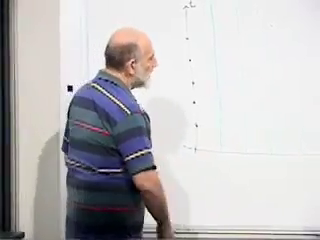
\includegraphics[width=0.62\textwidth]{lecture_01_figure_02.png}\caption{El eje temporal del sistema en reposo y las primeras líneas de universo de la retícula espacial.}\lectureframe{00:16:38}\end{figure}

La misma construcción se aprecia mejor en un dibujo idealizado:

\begin{figure}[H]\centering
\begin{tikzpicture}[scale=0.95]
\draw[->] (-1.2,0) -- (5.2,0) node[right] {$x$};
\draw[->] (0,-0.2) -- (0,4.8) node[above] {$t$};
\foreach \x in {-1,1,2,3,4}
  \draw[gray!65] (\x,0) -- (\x,4.4);
\foreach \y in {1,2,3,4}
  \draw[gray!65] (-1.0,\y) -- (4.4,\y);
\fill (0,0) circle (1.5pt);
\node[below left] at (0,0) {$0$};
\node[left] at (0,1) {$1$};
\node[left] at (0,2) {$2$};
\node[left] at (0,3) {$3$};
\node[below] at (1,0) {$1$};
\node[below] at (2,0) {$2$};
\node[below] at (3,0) {$3$};
\end{tikzpicture}\caption{Una retícula de espaciotiempo en reposo. Las líneas verticales tienen posición constante; las horizontales, tiempo constante.}\end{figure}

La retícula es imaginaria y su espaciado es arbitrario. Podemos usar metros, centímetros, micras o cualquier intervalo aún menor que tenga sentido físico. Su propósito es asignar una coordenada precisa a cada suceso.

La expresión «sistema de referencia» adquiere ahora un contenido operacional. No es simplemente un punto de vista ni una persona que mira en cierta dirección. Es un aparato de coordenadas extendido. Para un suceso dado, las reglas locales especifican dónde ocurrió y el reloj local indica cuándo. Así podemos comparar otras magnitudes físicas entre sistemas de referencia: la posición y la velocidad de una partícula, su energía, quizá la temperatura de un cuerpo y, más adelante, su momento lineal y su fuerza. La comparación más sencilla es la que involucra \(x\) y \(t\), así que empezaremos por ahí.

Coloquemos ahora una segunda retícula en un tren que se mueve en la dirección positiva de \(x\) con velocidad constante \(v\). Hagamos coincidir los orígenes en \(t=0\). Entonces, el origen móvil sigue la trayectoria
\begin{equation}
x=vt.
\end{equation}
Cada uno de los demás puntos fijos del tren sigue una línea de universo paralela e inclinada. Esa inclinación expresa geométricamente que el tren cambia de posición con el paso del tiempo.

Supongamos que el punto trasero del tren es el origen primado. En \(t=0\) coincide con el origen de la estación. En un tiempo posterior \(t\), su coordenada en reposo es \(vt\). Así pues, un suceso cercano de coordenada \(x\) está a solo \(x-vt\) del origen del tren. Por eso la transformación implica una resta y no una regla algebraica arbitraria.

Sean \((x,t)\) las coordenadas de un suceso en el sistema de referencia de la estación y \((x',t')\) sus coordenadas en el del tren. Galileo y Newton mantienen el tiempo universal:
\begin{equation}
t'=t.
\end{equation}
Durante el intervalo \(t\), el origen móvil avanza \(vt\), así que la distancia entre ese origen y el suceso es
\begin{equation}
x'=x-vt.
\end{equation}
En conjunto:
\begin{align}
t'&=t, & x'&=x-vt.
\label{eq:galilean-forward}
\end{align}
Al despejar las coordenadas no primadas, obtenemos la transformación inversa:
\begin{align}
t&=t', & x&=x'+vt'.
\label{eq:galilean-inverse}
\end{align}

\begin{figure}[H]\centering
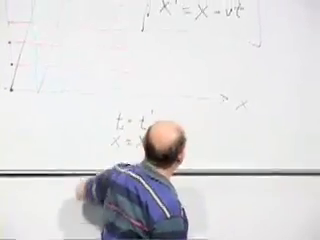
\includegraphics[width=0.72\textwidth]{lecture_01_figure_03.png}\caption{La transformación galileana escrita junto a las dos retículas del espaciotiempo.}\lectureframe{00:21:57}\end{figure}

El primer par indica al observador móvil cómo transformar las coordenadas proporcionadas por el observador en reposo. El par inverso transforma las coordenadas de vuelta. Esta conversión recíproca entre descripciones es el contenido matemático de la relatividad galileana.

La sustitución \(t\to t'\) en la fórmula espacial inversa solo es inocua porque la teoría galileana ya ha establecido que \(t=t'\). Conviene advertir esta hipótesis desde ahora. En la teoría de Einstein, las dos coordenadas temporales serán distintas, y estas sustituciones ya no serán automáticas.

\begin{classroomqa}\audiencequestion{Si se aleja un reloj y luego se lo trae de vuelta, ¿cómo podemos saber que el movimiento no lo aceleró primero y luego lo frenó, ocultando el efecto cuando se comparan los relojes?\lecturetimestamp{00:23:09}}\lecturerresponse{Galileo no podría haber establecido el tiempo universal con la precisión moderna; era una conjetura física. Podemos ponerla a prueba de muchas maneras: llevar buenos relojes en direcciones opuestas, repetir el viaje hacia el norte--sur y también hacia el este--oeste, mover un reloj alrededor del otro o intercambiar señales horarias sin reunir los relojes. A velocidades ordinarias, todas esas pruebas concuerdan con gran precisión. Si los relojes son lo bastante precisos o las velocidades lo bastante altas, aparece una pequeña discrepancia. Que falle la hipótesis del tiempo universal no significa que el experimento tenga un defecto; es uno de los fenómenos que la relatividad especial debe explicar.}\end{classroomqa}

\section{Invariantes galileanos y ley de Newton}

Un invariante es una magnitud en la que coinciden todos los observadores inerciales considerados. Las coordenadas no tienen por qué ser invariantes. Lo que importa es que las leyes formuladas con ellas conserven la misma forma.

El término se usa tanto como sustantivo como adjetivo. Un número puede ser un invariante y una ecuación puede ser invariante bajo una transformación. Distinguir entre magnitudes invariantes y leyes invariantes evita una confusión habitual: la relatividad no afirma que todos los observadores obtengan las mismas coordenadas para todo. Afirma que la ley física que relaciona sus mediciones tiene la misma forma.

Tomemos dos sucesos simultáneos en las posiciones \(x_1\) y \(x_2\). La ecuación~\eqref{eq:galilean-forward} da
\begin{align}
x_1'&=x_1-vt,\\
x_2'&=x_2-vt.
\end{align}
Por tanto, su separación es
\begin{equation}
x_2'-x_1'=(x_2-vt)-(x_1-vt)=x_2-x_1.
\end{equation}
En la física galileana, la distancia entre sucesos que ocurren al mismo tiempo es invariante, aunque las posiciones individuales no lo sean.

\begin{classroomqa}\audiencequestion{¿Las dos apariciones de \(t\) en esa resta se refieren realmente al mismo tiempo?\lecturetimestamp{00:28:16}}\lecturerresponse{Sí. Hemos elegido deliberadamente los dos sucesos \((x_1,t)\) y \((x_2,t)\). Están sobre una misma línea horizontal de tiempo constante. Por tanto, el término común \(vt\) se cancela. Si los sucesos ocurrieran en tiempos distintos, este razonamiento no demostraría que la separación espacial fuera invariante.}\end{classroomqa}

Describamos ahora una partícula mediante una trayectoria \(x(t)\). El observador del tren le asigna
\begin{equation}
x'(t)=x(t)-vt.
\end{equation}
Al derivar una vez, obtenemos la conocida regla de suma de velocidades:
\begin{equation}
\frac{dx'}{dt}=\frac{dx}{dt}-v.
\end{equation}
La posición y la velocidad dependen del sistema de referencia. Un observador que se desplaza junto a una flecha la ve moverse más despacio que otro situado junto a la vía.

Derivemos de nuevo. Como la velocidad relativa \(v\) es constante,
\begin{equation}
\frac{d^2x'}{dt^2}=\frac{d^2x}{dt^2}.
\end{equation}
La aceleración es invariante bajo una transformación galileana. Esto sugiere con fuerza por qué la ley de Newton se expresa en términos de aceleración y no de posición o velocidad.

Esta es la aceleración de un objeto observado, no la aceleración del observador del tren. Ambos sistemas son inerciales, así que ninguno acelera respecto del otro. Los objetos pueden acelerarse hacia la izquierda o la derecha en cualquiera de las dos descripciones, y los dos observadores coinciden en el valor de esa aceleración, aunque discrepen sobre la posición y la velocidad del objeto.

Supongamos que dos partículas ejercen una fuerza entre sí y que esta depende únicamente de su separación simultánea. Como esa separación es invariante, la fuerza también lo es. Si la masa es además una propiedad intrínseca, independiente del sistema de referencia, todo observador inercial puede escribir
\begin{equation}
F=ma
\end{equation}
exactamente de la misma forma. La mecánica newtoniana es invariante bajo las transformaciones galileanas. No es solo plausible: dentro del dominio de las velocidades ordinarias, es extraordinariamente precisa.

El razonamiento se aplica a fuerzas centrales conocidas, como la gravedad newtoniana o la fuerza electrostática, cuya magnitud depende de la distancia. Como todos los observadores galileanos coinciden en esa distancia en un mismo instante, también coinciden en la fuerza. Si la fuerza y la aceleración están fijadas, la consistencia exige entonces que coincidan también en la masa: un objeto de un kilogramo sigue teniendo un kilogramo cuando pasa en un tren. Todos los símbolos de \(F=ma\) encajan en la misma estructura invariante.

\section{La luz no obedece la regla galileana}

El electromagnetismo plantea la dificultad. Las ecuaciones de Maxwell predicen ondas que viajan por el espacio vacío a una velocidad definida \(c\). Si las ecuaciones de Maxwell son leyes de la naturaleza y estas son iguales en todos los sistemas inerciales, entonces todos los observadores inerciales deben obtener el mismo valor de \(c\).

La cinemática galileana predice otra cosa. En el sistema en reposo, un pulso de luz que se desplaza hacia la derecha satisface
\begin{equation}
x=ct.
\end{equation}
Al aplicar la transformación espacial, se obtiene
\begin{equation}
x'=x-vt=(c-v)t.
\end{equation}
Como \(t'=t\), el observador del tren mediría una velocidad de \(c-v\).

La contradicción puede expresarse con claridad. Si las ecuaciones de Maxwell conservan su forma, predicen \(c\) en el sistema primado. Si se conserva la transformación galileana, esta predice \(c-v\). Ambas no pueden ser exactas cuando \(v\ne0\).

Este resultado parece del todo natural si la luz se comporta como una onda ordinaria en un medio. Una barca que se mueve con respecto a una ola de agua mide una velocidad de onda relativa menor. Un oyente que se desplaza en aire en reposo mide una velocidad del sonido modificada por su movimiento respecto del aire. Por eso, los físicos del siglo XIX propusieron un estado de reposo privilegiado: un sistema del éter en el que las ecuaciones de Maxwell tuvieran su forma más sencilla y la luz se propagara a \(c\). Los experimentos concebidos para detectar el movimiento respecto de ese sistema privilegiado no encontraron ningún efecto correspondiente.

Había varias maneras de organizar los experimentos, pero todas buscaban comparar la propagación de la luz para observadores con distintos estados o direcciones de movimiento. Ninguna reveló el desplazamiento galileano esperado. El fracaso no fue una pequeña molestia técnica. Obligó a elegir entre el principio de relatividad, las ecuaciones de Maxwell y las nociones heredadas de espacio y tiempo.

Einstein abordó el conflicto de forma más directa. De joven, imaginó que perseguía una onda luminosa. Si pudiera alcanzarla, su patrón electromagnético oscilante quedaría inmóvil en el espacio, pero las ecuaciones de Maxwell no admiten una onda luminosa estacionaria así. Einstein decidió tomar como fundamentales la teoría de Maxwell y el principio de relatividad, y reconsiderar después las hipótesis ocultas en nuestras coordenadas.

La reconstrucción se basa en dos postulados:
\begin{enumerate}
\item Las leyes de la física tienen la misma forma en todos los sistemas inerciales.
\item La luz en el vacío tiene la misma velocidad \(c\) en todos los sistemas inerciales.
\end{enumerate}

El segundo postulado no puede coexistir con la transformación galileana. Debe cambiar algo más profundo que la regla de suma de velocidades. La elección más económica de Einstein es mantener ambos postulados y reconsiderar la ecuación galileana aparentemente inocua \(t'=t\).

\section{Sincronización de relojes distantes}

Las distancias espaciales pueden determinarse con reglas, pero para sincronizar relojes distantes hace falta una convención. Coloquemos dos relojes a la misma distancia de un observador situado en el punto medio. Cuando cada reloj de los extremos marque la hora acordada, hagamos que emita un destello. Si ambos destellos llegan juntos al punto medio, diremos que los relojes de los extremos están sincronizados. Si uno llega antes, ajustamos el reloj correspondiente y repetimos el procedimiento.

El término \emph{punto medio} se define usando las reglas ya dispuestas en ese sistema de referencia. Por tanto, la prueba contiene dos elementos distintos: igual distancia espacial a ambos extremos e igual tiempo de llegada de las señales. No se puede omitir ninguno. Al repetir el procedimiento por toda la retícula, se obtiene la familia de líneas horizontales de tiempo constante que Newton simplemente había supuesto.

Esta definición usa la luz porque el postulado le asigna la misma velocidad en todos los sistemas inerciales. Una vez aplicado el procedimiento a todos los pares de puntos vecinos, toda la retícula tiene una familia sincronizada de relojes.

Imaginemos ahora que una segunda retícula se mueve a través de la primera. En su propio sistema, el punto medio del aparato móvil sigue estando a mitad de camino entre sus dos extremos móviles. Sin embargo, respecto del aparato en reposo, se acerca a uno de los destellos entrantes y se aleja del otro. Los destellos emitidos simultáneamente según los relojes en reposo no llegan juntos al punto medio móvil. Como el observador móvil aplica la misma regla del punto medio y la luz, no puede considerar simultáneas esas emisiones. Cada sistema sincroniza sus propios relojes de manera coherente, pero las dos sincronizaciones discrepan.

No se trata de una ilusión óptica causada por el tiempo que tarda la luz en llegar. Cada observador sabe que la luz tarda en llegar y corrige ese tiempo usando la misma velocidad \(c\). La discrepancia persiste tras la corrección porque los observadores no eligen los mismos sucesos distantes como un par simultáneo. Lo relativo es la simultaneidad misma, no solo su apariencia.

\begin{classroomqa}\audiencequestion{¿Podríamos evitar esta conclusión sincronizando los relojes con sonido en lugar de con luz?\lecturetimestamp{00:49:03}}\lecturerresponse{El sonido sirve como señal de sincronización en un sistema donde el aire está en reposo, pero su velocidad medida no es la misma en todos los sistemas inerciales. Un tren abierto que se mueve en aire en reposo se desplaza respecto del medio que transmite el sonido, por lo que las señales sonoras hacia delante y hacia atrás no se comportan simétricamente en él. La luz es distinta por postulado: no hay ningún medio óptico detectable cuyo sistema de reposo privilegie a un observador. Por eso usamos luz y seguimos sus consecuencias.}\end{classroomqa}

La discrepancia cualitativa está clara. Ahora calcularemos con precisión qué sucesos considera simultáneos el observador móvil.

\section{Construcción con rayos de luz}

Para esta construcción, conviene elegir unidades tales que
\begin{equation}
c=1.
\end{equation}
Una unidad de distancia es entonces la distancia que recorre la luz en una unidad de tiempo: segundos luz junto con segundos, o años luz junto con años. El espacio y el tiempo tienen las mismas unidades, las velocidades son adimensionales y los rayos de luz aparecen a \(45^\circ\). Un rayo que se desplaza hacia la derecha satisface
\begin{equation}
x=t+d,
\end{equation}
mientras que uno que se desplaza hacia la izquierda satisface
\begin{equation}
x=-t+d'.
\end{equation}
Los dos rayos que pasan por el origen son sencillamente \(x=t\) y \(x=-t\). Las trayectorias temporales, correspondientes a objetos más lentos que la luz, quedan más cerca del eje vertical. Una trayectoria hipotética superlumínica quedaría más cerca del eje horizontal.

El ángulo del dibujo solo tiene sentido tras elegir estas unidades. En metros y segundos, un rayo de luz parecería casi horizontal, porque recorre aproximadamente \(3\times10^8\) metros en un segundo. Elegir segundos luz como unidad de distancia reescala el eje horizontal y hace visible la geometría causal.

Consideremos tres líneas de universo paralelas de la retícula móvil:
\begin{equation}
x=vt,\qquad x=vt+L,\qquad x=vt+2L.
\label{eq:moving-worldlines}
\end{equation}
La línea de universo central corresponde al observador que pone a prueba la simultaneidad entre los dos puntos exteriores. Los tres puntos se mueven uniformemente y mantienen su disposición relativa en el sistema primado.

\begin{figure}[H]\centering
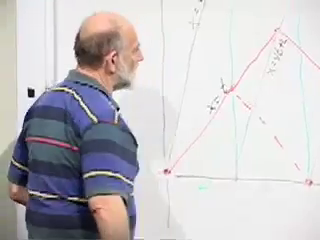
\includegraphics[width=0.72\textwidth]{lecture_01_figure_04.png}\caption{El rayo de luz hacia delante \(x=t\) que se encuentra con la línea de universo central móvil.}\lectureframe{01:02:33}\end{figure}

La geometría completa puede dibujarse sin que una persona de pie obstaculice la pizarra:

\begin{figure}[H]\centering
\begin{tikzpicture}[scale=0.95]
\draw[->] (-0.5,0) -- (6.5,0) node[right] {$x$};
\draw[->] (0,-0.2) -- (0,4.3) node[above] {$t$};
\draw[blue] (0,0) -- (1.4,4.0);
\draw[blue] (2.0,0) -- (3.4,4.0);
\draw[blue] (4.0,0) -- (5.4,4.0);
\draw[red] (0,0) -- (3.08,3.08);
\draw[red] (3.08,3.08) -- (4.56,1.60);
\draw[red,dashed] (2.0,0) -- (4.56,1.60);
\fill (0,0) circle (1.5pt);
\fill (2.0,0) circle (1.5pt);
\fill (4.0,0) circle (1.5pt);
\fill (3.08,3.08) circle (1.5pt);
\fill (4.56,1.60) circle (1.5pt);
\node[left] at (0.55,1.55) {$x=vt$};
\node[left] at (2.45,1.9) {$x=vt+L$};
\node[right] at (4.72,1.9) {$x=vt+2L$};
\node[left] at (1.88,2.28) {$x=t$};
\node[above right] at (3.08,3.08) {$A$};
\end{tikzpicture}\caption{Las señales luminosas determinan la línea de simultaneidad del sistema móvil.}\end{figure}

Enviemos desde el origen un rayo de luz hacia la derecha. Sea \(A\) la intersección con la línea de universo central. Las dos ecuaciones en \(A\) son
\begin{align}
x&=t,\\
x&=vt+L.
\end{align}
Al sustituir, obtenemos
\begin{equation}
t=vt+L,
\end{equation}
y, por tanto,
\begin{equation}
t_A=x_A=\frac{L}{1-v}.
\label{eq:point-a}
\end{equation}

Desde \(A\), tracemos hacia atrás un rayo de luz que se desplaza hacia la izquierda hasta la línea de universo móvil de la derecha. Su ecuación tiene la forma
\begin{equation}
x+t=b.
\end{equation}
Como pasa por \(A\), la ecuación~\eqref{eq:point-a} determina la constante:
\begin{equation}
b=x_A+t_A=\frac{2L}{1-v}.
\end{equation}
Así pues, el rayo hacia atrás satisface
\begin{equation}
x+t=\frac{2L}{1-v}.
\label{eq:backward-ray}
\end{equation}

La intersección con la línea de universo de la derecha se obtiene de
\begin{align}
x+t&=\frac{2L}{1-v},\\
x&=vt+2L.
\end{align}
Al eliminar \(x\),
\begin{align}
(1+v)t
  &=2L\left(\frac{1}{1-v}-1\right)\\
  &=\frac{2Lv}{1-v},
\end{align}
por lo que
\begin{equation}
t=\frac{2Lv}{1-v^2}.
\end{equation}
Al sustituir en \(x=vt+2L\), se obtiene
\begin{equation}
x=\frac{2L}{1-v^2}.
\end{equation}
Las coordenadas mismas importan menos que su cociente:
\begin{equation}
\frac{t}{x}=v.
\end{equation}
Por tanto, todos los sucesos simultáneos con el origen según los relojes móviles están en
\begin{equation}
t=vx,
\label{eq:simultaneity-c-one}
\end{equation}
mientras que el origen móvil sigue la trayectoria
\begin{equation}
x=vt.
\label{eq:moving-time-axis}
\end{equation}
Los dos ejes están inclinados simétricamente alrededor del rayo de luz a \(45^\circ\).

Todos los puntos de \(x=vt\) tienen la misma posición primada, \(x'=0\), mientras que sus tiempos primados varían. Todos los puntos de \(t=vx\) tienen el mismo tiempo primado, \(t'=0\), mientras que sus posiciones primadas varían. Por tanto, una línea es el eje temporal primado y la otra, el eje espacial primado. La larga construcción con señales era necesaria para determinar la segunda línea; no podía deducirse solo de la línea de universo móvil.

Para restablecer las unidades ordinarias en la ecuación~\eqref{eq:simultaneity-c-one}, hace falta
\begin{equation}
t=\frac{v}{c^2}x.
\label{eq:simultaneity-dimensional}
\end{equation}
El factor \(c^2\) explica por qué la imagen newtoniana funciona tan bien en la vida cotidiana. Para velocidades muy pequeñas en comparación con \(c\), la pendiente de la línea de simultaneidad móvil es ínfima.

\begin{figure}[H]\centering
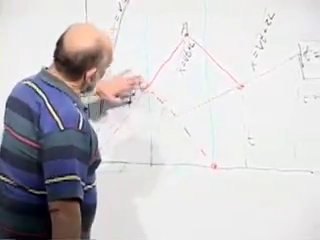
\includegraphics[width=0.72\textwidth]{lecture_01_figure_05.png}\caption{Con \(c=1\), los ejes primados temporal y de simultaneidad son simétricos respecto del rayo de luz.}\lectureframe{01:15:40}\end{figure}

\begin{figure}[H]\centering
\begin{tikzpicture}[scale=1.0]
\draw[->] (-2.2,0) -- (5.2,0) node[right] {$x$};
\draw[->] (0,-0.2) -- (0,4.9) node[above] {$t$};
\draw[red] (0,0) -- (3.9,3.9);
\draw[red] (0,0) -- (-1.8,1.8);
\draw[blue] (0,0) -- (1.8,4.5);
\draw[blue,dashed] (0,0) -- (4.5,1.8);
\node[right] at (3.9,3.9) {$x=t$};
\node[left] at (-1.8,1.8) {$x=-t$};
\node[above] at (1.8,4.5) {$x'=0$};
\node[right] at (4.5,1.8) {$t'=0$};
\end{tikzpicture}\caption{Los ejes primados y los rayos de luz invariantes en unidades \(c=1\).}\end{figure}

\section{Derivación de la transformación de Lorentz}

La geometría determina dónde se anula cada coordenada primada. Sobre el eje temporal móvil \(x=vt\), debe cumplirse \(x'=0\). Sobre el eje de simultaneidad móvil \(t=vx\), debe cumplirse \(t'=0\). Las relaciones lineales más generales que tienen esos conjuntos de ceros pueden escribirse así:
\begin{align}
x'&=\frac{x-vt}{F(v)},\\
t'&=\frac{t-vx}{G(v)}.
\label{eq:fg-ansatz}
\end{align}
Los factores \(F\) y \(G\) permiten que las escalas de las coordenadas primadas difieran de las galileanas, aunque ya hayamos determinado la ubicación de los ejes. La linealidad se desprende de la homogeneidad del espacio y el tiempo: trasladar un experimento no puede cambiar la ley de transformación.\editorialnote{Este breve argumento de linealidad hace explícita una hipótesis usada implícitamente en la derivación en la pizarra.}

En este punto, la geometría ya nos ha dicho mucho, pero no todo. Los numeradores fijan la inclinación de los ejes. No fijan la separación entre unidades a lo largo de ellos. Esa información de escala que aún falta es precisamente lo que representan \(F(v)\) y \(G(v)\).

Impongamos ahora que la velocidad de la luz sea invariante. Un rayo que se desplaza hacia la derecha y satisface \(x=t\) también debe satisfacer \(x'=t'\). A lo largo de ese rayo,
\begin{align}
x'&=\frac{(1-v)t}{F(v)},\\
t'&=\frac{(1-v)t}{G(v)}.
\end{align}
La igualdad para todos los puntos del rayo exige
\begin{equation}
F(v)=G(v).
\end{equation}
Por tanto, podemos escribir
\begin{align}
x'&=\frac{x-vt}{F(v)},\\
t'&=\frac{t-vx}{F(v)}.
\label{eq:common-f}
\end{align}

Este paso introduce en el álgebra la primera exigencia genuinamente einsteiniana. La misma línea geométrica es un rayo de luz para ambos observadores, así que las dos coordenadas primadas deben aumentar por igual a lo largo de ella cuando \(c=1\). Si los factores de las dos ecuaciones fueran distintos, la velocidad primada diferiría de la unidad.

Queda una función desconocida. Multipliquemos la ecuación~\eqref{eq:common-f} por \(F(v)\):
\begin{align}
F(v)x'&=x-vt,\\
F(v)t'&=t-vx.
\end{align}
Multiplicando la segunda ecuación por \(v\) y sumándola a la primera, eliminamos \(t\) y obtenemos
\begin{equation}
(1-v^2)x=F(v)(x'+vt').
\end{equation}
De manera análoga,
\begin{equation}
(1-v^2)t=F(v)(t'+vx').
\end{equation}
Por tanto, la transformación inversa es
\begin{align}
x&=\frac{F(v)}{1-v^2}(x'+vt'),\\
t&=\frac{F(v)}{1-v^2}(t'+vx').
\end{align}

El principio de relatividad hace recíprocos los dos sistemas. Si la estación ve que el tren se mueve a \(+v\), el tren ve que la estación se mueve a \(-v\). Por consiguiente, las ecuaciones inversas deben tener la misma forma que las directas, pero con el signo de \(v\) invertido. Sus factores prefactores deben satisfacer
\begin{equation}
\frac{F(v)}{1-v^2}=\frac{1}{F(v)}.
\end{equation}
Por tanto,
\begin{equation}
F(v)^2=1-v^2,
\end{equation}
y la continuidad con la transformación identidad en \(v=0\) selecciona la raíz positiva:
\begin{equation}
F(v)=\sqrt{1-v^2}.
\end{equation}

El resultado no se ha ajustado a ningún pulso luminoso particular. Se desprende de los ejes determinados por la sincronización, de que la velocidad de la luz es común y de la exigencia de que ninguno de los sistemas inerciales tenga un lugar privilegiado.

La transformación de Lorentz en unidades con \(c=1\) es
\begin{align}
x'&=\frac{x-vt}{\sqrt{1-v^2}},\\
t'&=\frac{t-vx}{\sqrt{1-v^2}}.
\label{eq:lorentz-c-one}
\end{align}
Su inversa es
\begin{align}
x&=\frac{x'+vt'}{\sqrt{1-v^2}},\\
t&=\frac{t'+vx'}{\sqrt{1-v^2}}.
\end{align}

\begin{figure}[H]\centering
\includegraphics[width=0.76\textwidth]{lecture_01_figure_06.png}\caption{La transformación de Lorentz \(c=1\) completa en la pizarra.}\lectureframe{01:32:38}\end{figure}

La novedad esencial ya se aprecia en la ecuación del tiempo. El tiempo no se traslada sin cambios de un sistema a otro. Una coordenada temporal primada combina tiempo y posición no primados. Por consiguiente, \(t=\text{constant}\) y \(t'=\text{constant}\) describen conjuntos distintos de sucesos.

El término de mezcla no es una corrección opcional añadida a posteriori. Sin él, la línea \(t'=0\) seguiría siendo horizontal, la simultaneidad distante continuaría siendo universal y la transformación no podría conservar la velocidad de la luz.

\section{Restablecer la velocidad de la luz y comprobar el resultado}

Cuando \(c\ne1\), la coherencia dimensional restituye los factores que faltaban. La razón \(v^2/c^2\) es adimensional, mientras que \((v/c^2)x\) tiene unidades de tiempo. Así pues,
\begin{align}
x'&=\frac{x-vt}{\sqrt{1-v^2/c^2}},\\
t'&=\frac{t-(v/c^2)x}{\sqrt{1-v^2/c^2}}.
\label{eq:lorentz-dimensional}
\end{align}
La transformación inversa se obtiene invirtiendo el signo de \(v\):
\begin{align}
x&=\frac{x'+vt'}{\sqrt{1-v^2/c^2}},\\
t&=\frac{t'+(v/c^2)x'}{\sqrt{1-v^2/c^2}}.
\end{align}
Si introducimos
\begin{equation}
\gamma=\frac{1}{\sqrt{1-v^2/c^2}}
\end{equation}
obtenemos la forma compacta habitual, pero escribir el denominador explícitamente permite seguir la derivación.

Numéricamente, \(c\simeq3\times10^8\,\mathrm{m/s}\), por lo que \(c^2\simeq9\times10^{16}\,\mathrm{m^2/s^2}\). El denominador grande hace que, en la mayoría de los experimentos mecánicos, la inclinación de la simultaneidad y el factor \(v^2/c^2\) sean imperceptibles. Que sean pequeños explica el éxito de Galileo; no restablece el tiempo absoluto.

\begin{figure}[H]\centering
\includegraphics[width=0.76\textwidth]{lecture_01_figure_07.png}\caption{La transformación de Lorentz tras restablecer los factores de \(c\).}\lectureframe{01:35:58}\end{figure}

Dos comprobaciones son inmediatas. Primero, consideremos \(v\ll c\). Entonces \(v^2/c^2\) es despreciable y, para distancias ordinarias, el término de relatividad de la simultaneidad \(vx/c^2\) también lo es. La ecuación~\eqref{eq:lorentz-dimensional} se reduce a
\begin{equation}
t'\approx t,\qquad x'\approx x-vt.
\end{equation}
Se recupera la relatividad galileana como aproximación a bajas velocidades.

Segundo, comprobemos el caso de un rayo de luz. Una vez restituido \(c\), un rayo que se propaga hacia la derecha satisface \(x=ct\), no \(x=t\). Al sustituir, se obtiene
\begin{align}
x'&=\frac{(c-v)t}{\sqrt{1-v^2/c^2}},\\
t'&=\frac{(1-v/c)t}{\sqrt{1-v^2/c^2}}.
\end{align}
Como \(c-v=c(1-v/c)\),
\begin{equation}
x'=ct'.
\end{equation}
El observador primado mide la misma velocidad \(c\). Para un rayo que se propaga hacia la izquierda, al sustituir \(x=-ct\) se obtiene, de manera análoga,
\begin{equation}
x'=-ct'.
\end{equation}
La transformación describe correctamente la luz que se propaga en cualquiera de las dos direcciones.

La distinción entre \(x=t\) y \(x=ct\) ofrece una comprobación dimensional instructiva. La primera expresión solo es correcta en unidades en las que \(c=1\). Restituir unidades ordinarias en la transformación y dejar la ecuación del rayo en unidades naturales mezclaría dos convenciones y daría un resultado erróneo. La coherencia dimensional permite detectar el error de inmediato.

\section{El criterio del punto medio}

\begin{classroomqa}
\audiencequestion{Supongamos que un observador recibe dos destellos en el mismo instante, pero no está a mitad de camino entre sus fuentes. ¿Puede concluir que los destellos se emitieron simultáneamente?
\lecturetimestamp{01:42:55}}
\lecturerresponse{No. Que los tiempos de llegada sean iguales implica que los tiempos de emisión también lo son únicamente para el observador situado espacialmente a mitad de camino entre las dos fuentes en el marco pertinente. Un receptor más cerca de una fuente puede recibir ambos destellos a la vez aunque el destello más lejano se haya emitido antes. En la construcción móvil, la línea de universo del punto medio \(x=vt+L\) es, por tanto, esencial. Se sigue el rayo que avanza \(x=t\) hasta que alcanza ese punto medio; luego se traza un rayo de luz hacia atrás hasta \(x=vt+2L\). Según el marco móvil, ese segundo suceso extremo es simultáneo con el origen; un suceso cualquiera de llegada simultánea en otro lugar no lo es.}
\end{classroomqa}

Hemos llegado a la transformación completa de coordenadas, pero todavía no a sus consecuencias más conocidas. A continuación veremos la contracción de la longitud, la dilatación del tiempo y el tiempo propio, y después el momento y la energía relativistas. Los fundamentos ya están establecidos: cada marco inercial puede emplear las mismas leyes y medir la misma velocidad de la luz solo porque el espacio y el tiempo se mezclan, y porque la simultaneidad a distancia depende del marco y no es absoluta.
\chapter{Ecuaciones de Maxwell, covariancia y ondas electromagnéticas}

\lectureoverview{Los campos eléctrico y magnético actúan sobre la materia cargada mediante la fuerza de Lorentz, pero la materia también debe crear y reorganizar los campos. Formularemos esa otra mitad recíproca del electromagnetismo, mostraremos que las ecuaciones de Maxwell son covariantes de Lorentz, deduciremos sus soluciones ondulatorias y, después, reincorporaremos la carga y la corriente en una forma que haga manifiesta la conservación local. A lo largo de la lección usaremos unidades en las que \(c=1\).}

\section{La otra mitad del electromagnetismo}

Empecemos por la parte del tema que ya conocemos. Si una partícula de carga \(q\) se mueve con velocidad \(\mathbf v\) a través de campos eléctricos y magnéticos, la fuerza es
\begin{equation}
\mathbf F=q\bigl(\mathbf E+\mathbf v\times\mathbf B\bigr).
\label{eq:lorentz-force-three}
\end{equation}
El factor \(q\) es indispensable. Una partícula sin carga no siente la fuerza electromagnética. El campo eléctrico contribuye incluso cuando la partícula está instantáneamente en reposo, mientras que la contribución magnética depende de su movimiento.

La ecuación~\eqref{eq:lorentz-force-three} nos dice qué efecto tienen sobre la materia unos campos dados. No nos dice qué determina esos campos. ¿Qué produce un campo eléctrico alrededor de un objeto, un campo magnético alrededor de otro o una onda que se propaga por el espacio vacío? Las ecuaciones que responden a esas preguntas son las ecuaciones de Maxwell.

\begin{figure}[H]
\centering
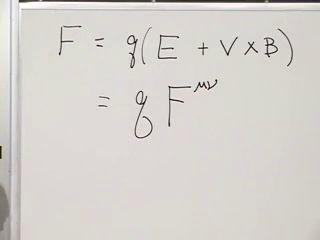
\includegraphics[width=0.62\textwidth]{lecture_58_figure_02.png}
\caption{La fuerza de Lorentz en forma de vector tridimensional y el comienzo de su reformulación tensorial.}
\lectureframe{00:05:49}
\end{figure}

La forma relativista de la ley de fuerza anticipa la notación que necesitaremos:
\begin{equation}
f^\mu=qF^\mu{}_{\nu}u^\nu.
\label{eq:lorentz-force-four}
\end{equation}
Aquí \(u^\nu\) es la cuadrivelocidad, \(f^\mu\) es la cuad fuerza y \(F^{\mu\nu}\) es un tensor antisimétrico construido a partir de \(\mathbf E\) y \(\mathbf B\). En la pizarra se muestra primero solo el comienzo esquemático de esta expresión; la contracción con \(u^\nu\) aporta el vector que falta para dejar un índice de fuerza libre.

Hay una razón física por la que la materia debe actuar también sobre el campo. Una onda electromagnética puede incidir sobre una carga, acelerarla y transferirle energía. Si el campo pudiera afectar a la carga, pero esta nunca pudiera afectar al campo, no habría ningún lugar del que pudiera provenir esa energía. La acción y la reacción no explican por sí solas todo el argumento, pero la conservación de la energía hace inevitable el acoplamiento recíproco.

\section{Una fuente cambiante emite una perturbación}

Una carga puntual produce un campo eléctrico dirigido hacia fuera o hacia dentro desde su posición. Una corriente en un hilo--un flujo de partículas cargadas--produce un campo magnético que circula alrededor del hilo. Estas conocidas imágenes estáticas muestran ya dos patrones geométricos distintos: el flujo eléctrico emana de la carga, mientras que las líneas del campo magnético rodean la corriente.

Ahora desplacemos bruscamente la carga puntual. Cerca de su nueva posición, el campo eléctrico debe empezar a reorganizarse, pero un observador lejano no puede enterarse del movimiento de manera instantánea. El campo antiguo persiste a gran distancia hasta que la señal tiene tiempo de llegar. Entre las regiones cercana y lejana hay un frente en movimiento donde el campo está cambiando. Esa reorganización en movimiento es una perturbación electromagnética.

Si la carga oscila de un lado a otro, las reorganizaciones sucesivas se siguen unas a otras y forman una onda electromagnética. Esta es la función básica de una antena: una corriente eléctrica oscilante envía hacia el exterior una perturbación del campo. Invertir una corriente en un hilo da la versión magnética del mismo argumento. La circulación de \(\mathbf B\) debe invertirse, pero la inversión se propaga en lugar de aparecer simultáneamente en todas partes.

Esta imagen causal fija dos objetivos para las ecuaciones de Maxwell. Deben describir cómo la carga y la corriente generan los campos y permitir que los cambios de esos campos se propaguen a una velocidad que no supere la de la luz. El segundo objetivo también pone a prueba la relatividad. Si las ecuaciones de Maxwell tienen la misma forma en todos los sistemas de referencia inerciales e implican una velocidad de onda definida, todos los observadores inerciales deben deducir de ellas la misma velocidad.

\section{Repaso de la ecuación de ondas relativista}

Antes de pasar a los campos vectoriales, consideremos un campo escalar \(\phi(\mathbf x,t)\), que asigna un número a cada punto del espacio-tiempo. Una ecuación con una derivada,
\begin{equation}
\partial_\mu\phi=0
\end{equation}
indicaría que todas las derivadas respecto del espacio-tiempo se anulan. El campo sería constante y, por tanto, no podría transportar una onda. Una ecuación de ondas relativista no trivial contiene dos derivadas:
\begin{equation}
\partial_\mu\partial^\mu\phi=0.
\end{equation}
Con la convención de signos que usamos aquí,
\begin{equation}
\left(\partial_t^2-\partial_x^2-\partial_y^2-\partial_z^2\right)\phi=0,
\label{eq:scalar-wave-four}
\end{equation}
o, de forma más compacta,
\begin{equation}
\left(\partial_t^2-\nabla^2\right)\phi=0.
\end{equation}
La elección \(c=1\) permite que el tiempo y la distancia tengan unidades compatibles. Al restablecer las unidades habituales, aparecería \(1/c^2\) junto a la segunda derivada temporal.

Para una onda que se propaga a lo largo del eje \(z\), el campo depende de \(z\) y \(t\), pero no de \(x\) ni de \(y\). La ecuación~\eqref{eq:scalar-wave-four} se reduce a
\begin{equation}
\left(\partial_t^2-\partial_z^2\right)\phi=0.
\label{eq:scalar-wave-one}
\end{equation}

\begin{figure}[H]
\centering
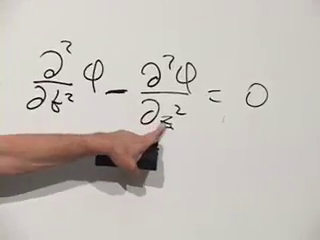
\includegraphics[width=0.56\textwidth]{lecture_58_figure_04.png}
\caption{La ecuación de ondas escalar unidimensional, usada como modelo para las ondas electromagnéticas.}
\lectureframe{00:47:03}
\end{figure}

Su forma general como onda viajera es
\begin{equation}
\phi(z,t)=f(z-t)+g(z+t).
\end{equation}
El perfil \(f(z-t)\) se desplaza hacia valores crecientes de \(z\), ya que un punto de fase constante satisface \(z-t=\text{constant}\). El perfil \(g(z+t)\) se desplaza en sentido contrario. Ninguno de los perfiles tiene por qué ser sinusoidal: cualquier forma suficientemente suave se traslada sin cambiar de forma.

Sin embargo, las funciones sinusoidales son prácticas:
\begin{equation}
\phi(z,t)=A\cos\!\bigl(k(z-t)\bigr).
\end{equation}
El número de onda \(k\) determina la longitud de onda,
\begin{equation}
\lambda=\frac{2\pi}{k}.
\end{equation}
Un valor grande de \(k\) produce oscilaciones espaciales rápidas y una longitud de onda corta; un valor pequeño de \(k\) produce una longitud de onda larga. Pronto, estos mismos perfiles pasarán a ser componentes de \(\mathbf E\) y \(\mathbf B\).

\section{El cálculo vectorial que necesita Maxwell}

Las ecuaciones de Maxwell se expresan mediante productos escalares, productos vectoriales, divergencias y rotacionales. Conviene repasar una vez esta notación, porque en los cálculos por componentes que siguen se usan exactamente estos patrones.

Para los vectores tridimensionales ordinarios \(\mathbf a\) y \(\mathbf b\), el producto escalar es el escalar
\begin{equation}
\mathbf a\cdot\mathbf b
=a_xb_x+a_yb_y+a_zb_z.
\end{equation}
El producto vectorial es otro vector,
\begin{align}
(\mathbf a\times\mathbf b)_x&=a_yb_z-a_zb_y,\\
(\mathbf a\times\mathbf b)_y&=a_zb_x-a_xb_z,\\
(\mathbf a\times\mathbf b)_z&=a_xb_y-a_yb_x.
\end{align}
Las demás componentes se obtienen siguiendo el orden cíclico \(x\to y\to z\to x\).

Introduzcamos el operador diferencial
\begin{equation}
\boldsymbol\nabla=
\left(\partial_x,\partial_y,\partial_z\right).
\end{equation}
Sus componentes son operadores y no números ordinarios, pero aun así pueden aplicarse los patrones del producto escalar y del producto vectorial. Para un campo vectorial \(\mathbf A\),
\begin{equation}
\boldsymbol\nabla\cdot\mathbf A
=\partial_xA_x+\partial_yA_y+\partial_zA_z
\label{eq:divergence}
\end{equation}
es la divergencia, mientras que
\begin{align}
(\boldsymbol\nabla\times\mathbf A)_x
 &=\partial_yA_z-\partial_zA_y,\\
(\boldsymbol\nabla\times\mathbf A)_y
 &=\partial_zA_x-\partial_xA_z,\\
(\boldsymbol\nabla\times\mathbf A)_z
 &=\partial_xA_y-\partial_yA_x
\label{eq:curl}
\end{align}
son las componentes del rotacional.

La geometría es tan importante como las fórmulas. Un campo vectorial tiene divergencia positiva donde parece fluir hacia fuera desde una fuente. Tiene rotacional donde circula. El campo eléctrico radial de una carga puntual ilustra la divergencia; el campo magnético que rodea un hilo por el que circula corriente ilustra el rotacional. Un campo vectorial espacialmente constante no tiene ninguno de los dos.

\section{Las ecuaciones de Maxwell en el vacío}

En ausencia de carga y corriente, las ecuaciones de Maxwell son
\begin{align}
\boldsymbol\nabla\times\mathbf E&=-\partial_t\mathbf B,
\label{eq:faraday-vac}\\
\boldsymbol\nabla\cdot\mathbf B&=0,
\label{eq:gauss-b-vac}\\
\boldsymbol\nabla\times\mathbf B&=\partial_t\mathbf E,
\label{eq:ampere-vac}\\
\boldsymbol\nabla\cdot\mathbf E&=0.
\label{eq:gauss-e-vac}
\end{align}
Las dos ecuaciones del rotacional casi intercambian \(\mathbf E\) y \(\mathbf B\), pero las distingue un signo menos esencial. Las dos ecuaciones de la divergencia indican que ninguno de los campos tiene fuentes en la región de vacío considerada. La divergencia magnética sigue siendo nula incluso cuando se reincorporan las fuentes eléctricas: el electromagnetismo ordinario no contiene carga magnética.

\begin{figure}[H]
\centering
\includegraphics[width=0.76\textwidth]{lecture_58_figure_06.png}
\caption{Las cuatro ecuaciones de Maxwell en el vacío, dispuestas para mostrar la simetría aproximada entre los campos eléctrico y magnético.}
\lectureframe{00:27:30}
\end{figure}

La densidad de carga \(\rho\) acabará sustituyendo al cero en el lado derecho de la ecuación~\eqref{eq:gauss-e-vac}, y la densidad de corriente \(\mathbf J\) aparecerá en la ecuación~\eqref{eq:ampere-vac}. Por ahora, dejamos esos términos de lado. Las ecuaciones sin fuentes ponen de manifiesto la estructura de transformación y el mecanismo de las ondas con el menor número de elementos que distraigan.

También agudizan el enigma de Einstein. Un observador galileano que siguiera una onda esperaría restar velocidades y medir una velocidad de onda menor. Sin embargo, si las mismas ecuaciones de Maxwell son válidas en todos los sistemas inerciales, cada observador deduce la misma velocidad de onda unitaria. La solución no consiste en modificar la ecuación de ondas de un sistema de referencia a otro. Consiste en usar la transformación de Lorentz y expresar las ecuaciones de Maxwell mediante objetos cuyas leyes de transformación ya conocemos.

\section{Los campos eléctrico y magnético como un solo tensor}

Los campos eléctrico y magnético se combinan en el tensor de campo antisimétrico
\begin{equation}
F^{\mu\nu}=
\begin{pmatrix}
0   & -E_x & -E_y & -E_z\\
E_x & 0    & -B_z & B_y\\
E_y & B_z  & 0    & -B_x\\
E_z & -B_y & B_x  & 0
\end{pmatrix},
\label{eq:l0203-field-tensor}
\end{equation}
donde el orden de filas y columnas es \(t,x,y,z\). La antisimetría,
\begin{equation}
F^{\mu\nu}=-F^{\nu\mu},
\end{equation}
obliga a que las entradas diagonales se anulen y determina la mitad inferior de la matriz a partir de la mitad superior. Las entradas espacio-temporales contienen \(\mathbf E\); las entradas puramente espaciales contienen \(\mathbf B\).

\begin{figure}[H]
\centering
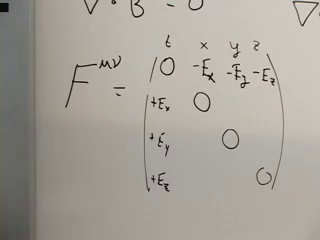
\includegraphics[width=0.58\textwidth]{lecture_58_figure_03.png}
\caption{El tensor de campo electromagnético completo, con sus componentes eléctricas y magnéticas.}
\lectureframe{00:32:05}
\end{figure}

La importancia de \(F^{\mu\nu}\) no reside solo en que sus seis componentes de campo quepan en una matriz. Se transforma como un tensor de rango dos bajo una transformación de Lorentz. Por tanto, los campos eléctrico y magnético que miden distintos observadores se mezclan exactamente de la manera necesaria para que el objeto completo se transforme de forma coherente.

Hay un segundo tensor antisimétrico: el tensor de campo dual \(\widetilde F^{\mu\nu}\). Con la convención actual, se obtiene de la ecuación~\eqref{eq:l0203-field-tensor} mediante el reemplazo
\begin{equation}
\mathbf E\longmapsto-\mathbf B,
\qquad
\mathbf B\longmapsto\mathbf E.
\label{eq:dual-replacement}
\end{equation}
Así,
\begin{equation}
\widetilde F^{\mu\nu}=
\begin{pmatrix}
0    & B_x  & B_y  & B_z\\
-B_x & 0    & -E_z & E_y\\
-B_y & E_z  & 0    & -E_x\\
-B_z & -E_y & E_x  & 0
\end{pmatrix}.
\label{eq:dual-tensor}
\end{equation}
El signo de la ecuación~\eqref{eq:dual-replacement} es importante. Primero, en la lección se intenta expresar verbalmente el intercambio, se detecta la discrepancia de signo y se corrige antes de completar la matriz.

\begin{figure}[H]
\centering
\includegraphics[width=0.58\textwidth]{lecture_58_figure_07.png}
\caption{Construcción del tensor dual mediante el intercambio de las componentes eléctricas y magnéticas con el signo requerido.}
\lectureframe{00:35:45}
\end{figure}

\section{Las ecuaciones covariantes en el vacío}

Cada ecuación de Maxwell contiene una derivada. Si contraemos un tensor de rango dos con una derivada, queda un índice libre, por lo que las opciones covariantes naturales son
\begin{align}
\partial_\mu F^{\mu\nu}&=0,
\label{eq:maxwell-covariant-vac}\\
\partial_\mu\widetilde F^{\mu\nu}&=0.
\label{eq:maxwell-dual-vac}
\end{align}
Para cada valor fijo de \(\nu\), la ecuación~\eqref{eq:maxwell-covariant-vac} es una ecuación. Como \(\nu\) puede tomar los valores \(t,x,y,z\), esta notación reúne cuatro ecuaciones escalares. La ecuación~\eqref{eq:maxwell-dual-vac} reúne las otras cuatro. Esto corresponde a las dos ecuaciones vectoriales del rotacional y a las dos ecuaciones escalares de la divergencia de la lista original.

La notación compacta solo es útil si reproduce las ecuaciones conocidas. Tomemos \(\nu=z\):
\begin{align}
\partial_\mu F^{\mu z}
&=\partial_tF^{tz}
  +\partial_xF^{xz}
  +\partial_yF^{yz}
  +\partial_zF^{zz}\\
&=-\partial_tE_z+\partial_xB_y-\partial_yB_x\\
&=-\partial_tE_z+
  \bigl(\boldsymbol\nabla\times\mathbf B\bigr)_z.
\end{align}
El término \(F^{zz}\) se anula por antisimetría. Al igualar a cero el resultado, obtenemos la componente \(z\) de
\begin{equation}
\boldsymbol\nabla\times\mathbf B=\partial_t\mathbf E.
\end{equation}
Las componentes \(x\) y \(y\) se obtienen mediante permutaciones cíclicas de los índices.

\begin{figure}[H]
\centering
\includegraphics[width=0.76\textwidth]{lecture_58_figure_08.png}
\caption{Desarrollo por componentes de la ecuación covariante de campo: la entrada diagonal del tensor se anula y los términos restantes reconstruyen las ecuaciones de Maxwell.}
\lectureframe{00:43:30}
\end{figure}

Ahora tomemos la componente temporal:
\begin{align}
\partial_\mu F^{\mu t}
&=\partial_tF^{tt}
  +\partial_xF^{xt}
  +\partial_yF^{yt}
  +\partial_zF^{zt}\\
&=\partial_xE_x+\partial_yE_y+\partial_zE_z\\
&=\boldsymbol\nabla\cdot\mathbf E.
\end{align}
Por tanto, da la ecuación~\eqref{eq:gauss-e-vac}. Al hacer las mismas comprobaciones con el tensor dual, se obtienen
\(\boldsymbol\nabla\cdot\mathbf B=0\) y
\(\boldsymbol\nabla\times\mathbf E=-\partial_t\mathbf B\).

Ahora las ecuaciones compactas están demostradas, no solo conjeturadas. Su estructura con índices libres las convierte en ecuaciones de cuadrivectores, de modo que una transformación de Lorentz cambia sus componentes, pero no su forma. Este es el sentido preciso en que las ecuaciones de Maxwell en el vacío son iguales en todos los sistemas de referencia inerciales.

\section{De las ecuaciones de primer orden a una onda}

Las ecuaciones de Maxwell contienen solo derivadas de primer orden, mientras que una ecuación de ondas contiene derivadas de segundo orden. La aparente discrepancia se resuelve porque la teoría de Maxwell acopla dos campos. Un par de ecuaciones de primer orden para \(\mathbf E\) y \(\mathbf B\) puede combinarse para obtener una ecuación de segundo orden para cualquiera de los dos campos por separado.

Derivemos la ecuación~\eqref{eq:ampere-vac} respecto del tiempo:
\begin{equation}
\partial_t^2\mathbf E
=\boldsymbol\nabla\times\partial_t\mathbf B.
\end{equation}
La ley de Faraday proporciona la derivada temporal de \(\mathbf B\):
\begin{equation}
\partial_t\mathbf B=-\boldsymbol\nabla\times\mathbf E,
\end{equation}
y, por tanto,
\begin{equation}
\partial_t^2\mathbf E
=-\boldsymbol\nabla\times
  \bigl(\boldsymbol\nabla\times\mathbf E\bigr).
\label{eq:double-curl}
\end{equation}

En la pizarra se desarrolla una componente en lugar de recurrir a una identidad memorizada. Para la componente \(x\),
\begin{align}
\bigl[\boldsymbol\nabla\times
(\boldsymbol\nabla\times\mathbf E)\bigr]_x
&=\partial_y(\boldsymbol\nabla\times\mathbf E)_z
 -\partial_z(\boldsymbol\nabla\times\mathbf E)_y\\
&=\partial_y(\partial_xE_y-\partial_yE_x)\\
&\quad-\partial_z(\partial_zE_x-\partial_xE_z)\\
&=\partial_x(\partial_yE_y+\partial_zE_z)
 -\partial_y^2E_x\\
&\quad-\partial_z^2E_x.
\end{align}
Sumemos y restemos \(\partial_x^2E_x\) para poner de manifiesto la divergencia:
\begin{align}
\bigl[\boldsymbol\nabla\times
(\boldsymbol\nabla\times\mathbf E)\bigr]_x
&=\partial_x(\boldsymbol\nabla\cdot\mathbf E)
 -\nabla^2E_x.
\label{eq:double-curl-x}
\end{align}
En el vacío, \(\boldsymbol\nabla\cdot\mathbf E=0\). Al combinar las ecuaciones~\eqref{eq:double-curl} y \eqref{eq:double-curl-x}, obtenemos
\begin{equation}
\left(\partial_t^2-\nabla^2\right)E_x=0.
\label{eq:ex-wave}
\end{equation}

\begin{figure}[H]
\centering
\includegraphics[width=0.72\textwidth]{lecture_58_figure_09.png}
\caption{El cálculo por componentes llega a la ecuación de ondas para \(E_x\).}
\lectureframe{00:57:10}
\end{figure}

El mismo cálculo se aplica a \(E_y\) y \(E_z\), y una eliminación análoga da
\begin{equation}
\left(\partial_t^2-\nabla^2\right)\mathbf B=0.
\end{equation}
Por tanto, los campos eléctrico y magnético pueden propagarse como ondas por el espacio vacío. En las unidades que usamos, su velocidad es uno; al restablecer las unidades habituales, esto significa que la velocidad es \(c\).

\section{Una onda plana y su polarización}

Construyamos una onda sencilla que se propague en la dirección positiva de \(z\):
\begin{equation}
\mathbf E(z,t)
=\widehat{\mathbf x}\,E_0
  \cos\!\bigl(k(z-t)\bigr).
\label{eq:plane-e}
\end{equation}
Su perfil se traslada a lo largo de \(z\) sin cambiar de forma. Como el campo eléctrico apunta a lo largo del eje \(x\), la onda está polarizada linealmente en la dirección \(x\). Hemos elegido \(E_y=0\) solo para mantener sencillo el ejemplo; podría incluirse una segunda polarización transversal.

La componente longitudinal no es igual de libre. Como la onda depende solo de \(z\) y \(t\),
\begin{equation}
\boldsymbol\nabla\cdot\mathbf E
=\partial_zE_z=0.
\end{equation}
Así, \(E_z\) puede ser constante, pero no puede contener el perfil ondulatorio variable. Puede superponerse o eliminarse por separado un campo de fondo uniforme; este no forma parte de la radiación que se propaga. La onda en sí es transversal:
\begin{equation}
\mathbf E_{\mathrm{wave}}\cdot\widehat{\mathbf z}=0.
\end{equation}

La ley de Faraday determina el campo magnético. Para la ecuación~\eqref{eq:plane-e}, la única componente no nula de \(\boldsymbol\nabla\times\mathbf E\) es la componente \(y\):
\begin{equation}
(\boldsymbol\nabla\times\mathbf E)_y=\partial_zE_x.
\end{equation}
En consecuencia, \(\partial_t\mathbf B\) apunta en la dirección \(y\), y una elección compatible es
\begin{equation}
\mathbf B(z,t)
=\widehat{\mathbf y}\,E_0
  \cos\!\bigl(k(z-t)\bigr).
\label{eq:plane-b}
\end{equation}
En estas unidades, las amplitudes eléctrica y magnética son iguales. Su orientación satisface
\begin{equation}
\mathbf E\perp\mathbf B,
\qquad
\mathbf E\perp\widehat{\mathbf z},
\qquad
\mathbf B\perp\widehat{\mathbf z},
\qquad
\mathbf E\times\mathbf B\parallel\widehat{\mathbf z}.
\end{equation}

\begin{figure}[H]
\centering
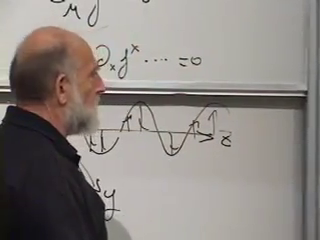
\includegraphics[width=0.70\textwidth]{lecture_58_figure_05.png}
\caption{Esquema completo de la pizarra de una onda electromagnética transversal: las oscilaciones de los campos eléctrico y magnético son perpendiculares entre sí y a la dirección de propagación.}
\lectureframe{01:05:25}
\end{figure}

\begin{figure}[H]
\centering
\scalebox{0.90}{%
\begin{tikzpicture}[x=1cm,y=1cm,>=Latex]
  \draw[->,thick] (0,0) -- (8.2,0) node[right] {$z$};
  \draw[->,thick] (0,-1.6) -- (0,1.7) node[above] {$x$};
  \draw[->,thick] (0,0) -- (-1.15,-0.8) node[below left] {$y$};
  \draw[blue!70!black,thick,domain=0:7.5,samples=120]
    plot (\x,{0.95*sin(90*\x)});
  \foreach \z/\s in {0.8/1,2.8/-1,4.8/1,6.8/-1}{
    \draw[->,green!45!black,thick]
      (\z,0) -- ++({-0.55*\s},{-0.38*\s});
  }
  \node[blue!70!black] at (6.9,1.25) {$\mathbf E$};
  \node[green!45!black] at (5.2,-1.05) {$\mathbf B$};
  \draw[->,very thick] (6.2,1.55) -- (7.7,1.55)
    node[midway,above] {propagation};
\end{tikzpicture}
}
\caption{Los campos \(\mathbf E\) y \(\mathbf B\) son perpendiculares entre sí y a la dirección de propagación.}
\end{figure}

Esta es la naturaleza de la luz y de toda radiación electromagnética en el vacío. Como las ecuaciones que producen la onda son covariantes de Lorentz, otro observador inercial describe, a su vez, una onda electromagnética que se propaga a \(c\), con campos eléctrico y magnético transversales.

\section{Densidad de carga y densidad de corriente}

Ahora reincorporamos las fuentes que habíamos dejado temporalmente de lado. Cuando una región contiene muchas partículas cargadas, resulta útil aproximarlas como una densidad de carga continua
\begin{equation}
\rho(\mathbf x,t)=\frac{dQ}{dV}.
\end{equation}
La aproximación es similar a tratar el agua como un fluido continuo, aunque esté formada por moléculas. Las cargas positivas y negativas contribuyen con signos opuestos, por lo que \(\rho\) es la carga neta por unidad de volumen.

La carga en una región elegida \(V\) es
\begin{equation}
Q_V(t)=\int_V\rho(\mathbf x,t)\,dV.
\label{eq:charge-volume}
\end{equation}
La densidad puede variar con la posición y el tiempo. Una acumulación de carga puede alejarse de un punto y cambiar allí la densidad local. Sin embargo, esta no puede variar de forma arbitraria. La naturaleza conserva la carga eléctrica.

La conservación global por sí sola sería demasiado débil. Permitiría que la carga desapareciera de la Tierra y reapareciera en Marte en el mismo instante, siempre que el total no cambiara. La afirmación más fuerte es local: la carga solo puede salir de un lugar y llegar a otro si fluye por el espacio intermedio.

Para describir ese flujo, tomemos un elemento de superficie infinitesimal orientado
\begin{equation}
d\boldsymbol\sigma=\widehat{\mathbf n}\,d\sigma.
\end{equation}
Su módulo es el área y su dirección es normal a la superficie. La densidad de corriente \(\mathbf J\) se define de modo que la carga que atraviesa el elemento por unidad de tiempo sea
\begin{equation}
\frac{dQ}{dt}=\mathbf J\cdot d\boldsymbol\sigma.
\label{eq:current-flux-element}
\end{equation}
El módulo de \(\mathbf J\) es la carga por unidad de área y por unidad de tiempo, y su dirección es la del flujo de carga positiva.

\begin{figure}[H]
\centering
\includegraphics[width=0.64\textwidth]{lecture_58_figure_10.png}
\caption{Un elemento de área orientado y el factor de flujo \(d\boldsymbol\sigma\cdot\mathbf J\).}
\lectureframe{01:18:15}
\end{figure}

El producto escalar selecciona la componente normal a la superficie. Una corriente tangente a la superficie no atraviesa ninguno de sus lados y aporta cero. Una corriente paralela a la normal da el flujo máximo para un módulo fijo. La corriente en un hilo es un caso particular, pero \(\mathbf J\) también puede describir carga que fluye a través de una lámina o por todo el espacio tridimensional.

\section{Conservación local y ecuación de continuidad}

Fijemos una región \(V\) del espacio y orientemos hacia fuera cada elemento de su frontera cerrada \(\partial V\). Si hay una corriente neta saliente, la carga en el interior disminuye:
\begin{equation}
\frac{dQ_V}{dt}
=-\oint_{\partial V}\mathbf J\cdot d\boldsymbol\sigma.
\label{eq:integral-conservation}
\end{equation}
El signo menos tiene un significado físico, no es una convención: el flujo positivo saliente extrae carga positiva de la región. Usando la ecuación~\eqref{eq:charge-volume},
\begin{equation}
\int_V\partial_t\rho\,dV
=-\oint_{\partial V}\mathbf J\cdot d\boldsymbol\sigma.
\label{eq:integral-continuity-one}
\end{equation}

\begin{figure}[H]
\centering
\includegraphics[width=0.72\textwidth]{lecture_58_figure_11.png}
\caption{Ley de conservación para una región fija, una vez convertido el flujo superficial en una expresión de volumen.}
\lectureframe{01:29:00}
\end{figure}

El teorema de Gauss, también llamado teorema de la divergencia, relaciona el flujo a través de una superficie cerrada con la divergencia en su interior:
\begin{equation}
\oint_{\partial V}\mathbf A\cdot d\boldsymbol\sigma
=\int_V\boldsymbol\nabla\cdot\mathbf A\,dV.
\label{eq:divergence-theorem}
\end{equation}
Podemos imaginar tuberías ocultas que inyectan agua en distintos puntos del interior de un recipiente. La divergencia mide la tasa local a la que el agua sale de los extremos de las tuberías; la integral de superficie mide la cantidad total de agua que sale del recipiente. Todo lo que se genera como flujo saliente en el interior debe acabar atravesando la frontera.

Al aplicar la ecuación~\eqref{eq:divergence-theorem} a \(\mathbf J\), obtenemos
\begin{equation}
\int_V
\left(\partial_t\rho+\boldsymbol\nabla\cdot\mathbf J\right)dV=0.
\end{equation}
Esta relación es válida para cualquier región \(V\) posible. Por tanto, el integrando debe anularse punto por punto:
\begin{equation}
\boxed{\partial_t\rho+\boldsymbol\nabla\cdot\mathbf J=0.}
\label{eq:continuity-three}
\end{equation}

\begin{figure}[H]
\centering
\includegraphics[width=0.72\textwidth]{lecture_58_figure_12.png}
\caption{La ecuación de continuidad local escrita componente por componente.}
\lectureframe{01:29:50}
\end{figure}

La ecuación~\eqref{eq:continuity-three} expresa exactamente lo que exige la conservación local. Si la densidad de carga disminuye en un punto o en una región pequeña, la corriente debe divergir hacia fuera de allí. Si la corriente converge hacia dentro, la densidad de carga aumenta.

La densidad y la corriente forman de manera natural la cuadr corriente
\begin{equation}
J^\mu=(\rho,J_x,J_y,J_z)
\label{eq:four-current}
\end{equation}
en unidades \(c=1\). La ecuación de continuidad se convierte en la ecuación escalar de Lorentz
\begin{equation}
\partial_\mu J^\mu=0.
\label{eq:continuity-four}
\end{equation}
El flujo de una distribución relativista debe transformarse como un cuadrivector, igual que la cuadrivelocidad de una partícula. La ecuación~\eqref{eq:continuity-four} hace que la conservación local de la carga sea válida en todos los sistemas de referencia inerciales.

\section{Las ecuaciones de Maxwell con fuentes}

Al reincorporar la carga y la corriente, obtenemos
\begin{align}
\boldsymbol\nabla\cdot\mathbf E&=\rho,
\label{eq:gauss-e-source}\\
\boldsymbol\nabla\cdot\mathbf B&=0,\\
\boldsymbol\nabla\times\mathbf E&=-\partial_t\mathbf B,\\
\boldsymbol\nabla\times\mathbf B&=\partial_t\mathbf E+\mathbf J.
\label{eq:ampere-source}
\end{align}
Las ecuaciones que incluyen fuentes eléctricas se condensan en
\begin{equation}
\boxed{\partial_\mu F^{\mu\nu}=J^\nu,}
\label{eq:maxwell-source-covariant}
\end{equation}
mientras que el par magnético sin fuentes sigue siendo
\begin{equation}
\boxed{\partial_\mu\widetilde F^{\mu\nu}=0.}
\label{eq:maxwell-dual-source}
\end{equation}

\begin{figure}[H]
\centering
\includegraphics[width=0.78\textwidth]{lecture_58_figure_13.png}
\caption{Las ecuaciones de Maxwell con fuentes, junto a su forma covariante \(\partial_\mu F^{\mu\nu}=J^\nu\).}
\lectureframe{01:34:00}
\end{figure}

La componente temporal de la ecuación~\eqref{eq:maxwell-source-covariant} se escribe
\begin{equation}
\partial_\mu F^{\mu t}=J^t=\rho,
\end{equation}
y el cálculo por componentes que ya realizamos transforma su lado izquierdo en
\(\boldsymbol\nabla\cdot\mathbf E\). Las tres componentes espaciales reproducen
\(\boldsymbol\nabla\times\mathbf B=\partial_t\mathbf E+\mathbf J\).

Hay también una comprobación útil de consistencia. Al aplicar \(\partial_\nu\) a la ecuación~\eqref{eq:maxwell-source-covariant}, obtenemos
\begin{equation}
\partial_\nu J^\nu
=\partial_\nu\partial_\mu F^{\mu\nu}=0,
\end{equation}
porque las dos derivadas son simétricas bajo el intercambio \(\mu\leftrightarrow\nu\), mientras que \(F^{\mu\nu}\) es antisimétrico.\editorialnote{Esta breve comprobación de consistencia se deduce de la ecuación covariante y hace explícito por qué las ecuaciones de Maxwell con fuentes respetan automáticamente la ecuación de continuidad.}

La estructura recíproca ya está completa. La ley tensorial de fuerza
\(f^\mu=qF^\mu{}_\nu u^\nu\)
describe cómo actúan los campos sobre la carga, y la ecuación~\eqref{eq:maxwell-source-covariant} describe cómo la carga y la corriente generan campos. Ambas son ecuaciones tensoriales. En el vacío, las mismas ecuaciones de campo dan lugar a ondas transversales que se propagan a \(c\). Así, la covariancia de Lorentz y la ecuación de ondas electromagnéticas se encuentran en el punto que motivó esta construcción: todos los observadores inerciales obtienen las mismas leyes del electromagnetismo y la misma velocidad de la luz.

\chapter{Tiempo propio, dilatación temporal y contracción de la longitud}

A menudo elegiremos unidades en las que la velocidad de la luz sea $c=1$. En esas unidades, un año de tiempo y un año luz de distancia pueden compararse directamente, y las fórmulas son mucho más fáciles de leer. Siempre que $c$ tenga importancia física, volveremos a incluirlo. Basta con el análisis dimensional para determinar dónde va.

\section{La cuadrícula galileana del espacio-tiempo}

Comencemos con la relación anterior a Einstein entre un sistema en reposo y un tren que se mueve con velocidad $v$ a lo largo del eje $x$:
\begin{align}
x' &= x-vt, & t'&=t.
\label{eq:l4-galilean}
\end{align}
La segunda ecuación contiene la hipótesis newtoniana del tiempo universal. Todos los observadores usan las mismas superficies de simultaneidad, aunque sus orígenes espaciales se muevan unos respecto de otros.

Supongamos que el observador sin primas está junto a las vías y que el observador con primas viaja en el tren. El origen del tren tiene $x'=0$, así que su línea de universo en las coordenadas sin primas es
\begin{equation}
x=vt.
\end{equation}
Esa línea inclinada es el eje $t'$. En cambio, $t'=t$ indica que todas las líneas de $t'$ constante son las mismas líneas horizontales que las de $t$ constante.

\begin{figure}[H]
\centering
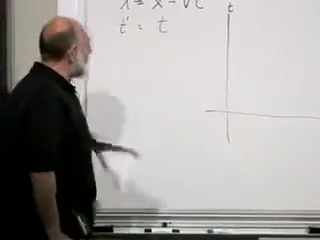
\includegraphics[width=0.72\textwidth]{lecture_04_figure_02.png}
\caption{La transformación galileana y la cuadrícula inicial de $t$-$x$. El origen móvil trazará $x=vt$, mientras los dos sistemas conservan en común las líneas de tiempo constante.}
\lectureframe{00:03:06}
\end{figure}

Al despejar las coordenadas sin primas en la ec.~\eqref{eq:l4-galilean} se obtiene
\begin{align}
x&=x'+vt'=x'+vt, & t&=t'.
\end{align}
La transformación inversa tiene la misma forma, pero con $v$ sustituido por $-v$. Si el tren avanza respecto de la estación, esta se mueve hacia atrás respecto del tren. Esta reciprocidad se conserva en la relatividad especial, pero el tiempo universal no.

\section{La corrección de Lorentz}

Las transformaciones galileanas no pueden hacer que la velocidad de la luz sea la misma en todos los sistemas inerciales. Las relaciones corregidas son, primero, en unidades de $c=1$,
\begin{align}
x'&=\frac{x-vt}{\sqrt{1-v^2}}, &
t'&=\frac{t-vx}{\sqrt{1-v^2}}.
\label{eq:l4-lorentz-natural}
\end{align}
Al volver a las unidades habituales se obtiene
\begin{align}
x'&=\frac{x-vt}{\sqrt{1-v^2/c^2}}, &
t'&=\frac{t-vx/c^2}{\sqrt{1-v^2/c^2}}.
\label{eq:l4-lorentz-c}
\end{align}

\begin{figure}[H]
\centering
\includegraphics[width=0.74\textwidth]{lecture_04_figure_05.png}
\caption{La transformación de Lorentz con los factores de $c$ restituidos.}
\lectureframe{00:09:10}
\end{figure}

Para $v\ll c$, tanto $v^2/c^2$ como $vx/c^2$ son pequeños en las circunstancias en que se usa la mecánica newtoniana. Entonces, la ec.~\eqref{eq:l4-lorentz-c} se reduce al resultado galileano. La relatividad no descarta la cinemática newtoniana; determina el rango en que es válida.

Para $v=c$, el denominador se anula. Un sistema inercial no puede moverse a la velocidad de la luz respecto de otro sistema inercial. Muy por debajo de ese límite las correcciones son pequeñas, pero cerca de él la mezcla de $x$ y $t$ se vuelve inevitable.

El movimiento se eligió a lo largo de $x$, así que las coordenadas transversales no cambian:
\begin{equation}
y'=y,\qquad z'=z.
\end{equation}
Una forma de entender por qué es colocar reglas transversales idénticas en el tren y en el andén. Un observador que se mueve a mitad de camino entre los dos sistemas ve las reglas acercarse con velocidades iguales y opuestas. En la situación no hay nada que pueda hacer que una regla transversal sea más corta que la otra.

\section{Transformaciones de Lorentz a lo largo del cono de luz}

La ec.~\eqref{eq:l4-lorentz-natural} puede interpretarse geométricamente. Sumemos sus dos ecuaciones:
\begin{align}
t'+x'
&=\frac{(t-vx)+(x-vt)}{\sqrt{1-v^2}}\\
&=(t+x)\frac{1-v}{\sqrt{1-v^2}}\\
&=(t+x)\sqrt{\frac{1-v}{1+v}}.
\label{eq:l4-null-plus}
\end{align}
Restémoslas en el orden complementario:
\begin{align}
t'-x'
&=\frac{(t-vx)-(x-vt)}{\sqrt{1-v^2}}\\
&=(t-x)\frac{1+v}{\sqrt{1-v^2}}\\
&=(t-x)\sqrt{\frac{1+v}{1-v}}.
\label{eq:l4-null-minus}
\end{align}

\begin{figure}[H]
\centering
\includegraphics[width=0.75\textwidth]{lecture_04_figure_06.png}
\caption{La transformación de Lorentz expresada mediante las combinaciones nulas $t+x$ y $t-x$. Sus factores de escala son recíprocos.}
\lectureframe{00:18:45}
\end{figure}

Las combinaciones $t+x$ y $t-x$ son coordenadas a lo largo de las dos direcciones $45^\circ$ luminosas. Un impulso de Lorentz comprime una de estas direcciones y estira la otra por el factor inverso. No rota ninguna de ellas fuera de $45^\circ$. Por tanto, los rayos de luz siguen siendo rayos de luz, lo que representa en el espacio-tiempo la invariancia de la velocidad de la luz.

\begin{classroomqa}\audiencequestion{El observador a mitad de camino ve un experimento simétrico, pero ¿cómo demuestra eso el resultado para los observadores del tren y del andén?
\lecturetimestamp{00:20:48}}\lecturerresponse{Se usa además un hecho: la coincidencia de dos sucesos es invariante. Si se encuentran los extremos de las reglas, ese encuentro es un único suceso del espacio-tiempo. Cada observador inercial puede asignarle coordenadas distintas, pero ninguno puede dividir una coincidencia en dos lugares diferentes. Los destellos emitidos donde se encuentran los extremos correspondientes permiten detectar esos sucesos de forma operacional. La simetría del sistema a mitad de camino y la invariancia de las coincidencias entre los dos pares de extremos demuestran que las longitudes transversales son iguales.}
\end{classroomqa}

\begin{classroomqa}\audiencequestion{¿El ciclista que representa el sistema de referencia a mitad de camino debe estar situado físicamente en el punto medio de las reglas?
\lecturetimestamp{00:22:25}}\lecturerresponse{No. Un sistema de referencia es una red completa de observadores y relojes, no un solo ojo en un lugar. El ciclista puede recibir después los destellos de los extremos e inferir dónde se originaron. Lo que importa es la ubicación en el espacio-tiempo de cada suceso de emisión, no dónde se recibe finalmente la luz.}
\end{classroomqa}

La composición de velocidades sucesivas es otra consecuencia de la misma transformación, pero se deja deliberadamente para la próxima clase. La tarea de hoy es identificar la cantidad invariante que mide un reloj en movimiento.

\section{El intervalo invariante}

En una rotación de los ejes cartesianos ordinarios, la cantidad $x^2+y^2$ no cambia. Las transformaciones de Lorentz conservan otra forma cuadrática. A partir de la ec.~\eqref{eq:l4-lorentz-natural},
\begin{align}
t'^2-x'^2
&=\frac{(t-vx)^2-(x-vt)^2}{1-v^2}\\
&=\frac{t^2-2vtx+v^2x^2-x^2+2vtx-v^2t^2}{1-v^2}\\
&=t^2-x^2.
\label{eq:l4-interval}
\end{align}
Los términos mixtos se cancelan y en el numerador restante aparece un factor común $1-v^2$.

\begin{figure}[H]
\centering
\includegraphics[width=0.76\textwidth]{lecture_04_figure_07.png}
\caption{La derivación en la pizarra de $t'^2-x'^2=t^2-x^2$.}
\lectureframe{00:33:15}
\end{figure}

En tres dimensiones espaciales, el invariante es
\begin{equation}
t'^2-x'^2-y'^2-z'^2=t^2-x^2-y^2-z^2
\end{equation}
en unidades de $c=1$. En general, para dos sucesos usamos diferencias de coordenadas:
\begin{equation}
\Delta s^2
=c^2\Delta t^2-\Delta x^2-\Delta y^2-\Delta z^2.
\label{eq:l4-spacetime-interval}
\end{equation}
Todos los observadores inerciales coinciden en este número, aunque discrepen sobre sus términos separados de tiempo y espacio.

\section{Tiempo propio y relojes en movimiento}

Imaginemos una red de observadores en reposo cuyos relojes se han sincronizado intercambiando señales luminosas. Sus lecturas definen el tiempo coordenado $t$. Ahora llevemos un reloj de pulsera a través de esa red. Su propia lectura acompaña al reloj a lo largo de su línea de universo; esa lectura es el tiempo propio.

Para dos sucesos separados temporalmente, definimos
\begin{equation}
c^2\Delta\tau^2
=c^2\Delta t^2-\Delta x^2-\Delta y^2-\Delta z^2.
\label{eq:l4-proper-time}
\end{equation}
En una dimensión espacial y con $c=1$, esto es simplemente
\begin{equation}
\Delta\tau=\sqrt{\Delta t^2-\Delta x^2}.
\end{equation}
La raíz cuadrada es análoga a la fórmula de la distancia ordinaria, pero el signo menos cambia la geometría.

Hay tres casos:
\begin{align}
\Delta t^2-\Delta x^2 &>0 &&\text{timelike},\\
\Delta t^2-\Delta x^2 &=0 &&\text{lightlike},\\
\Delta t^2-\Delta x^2 &<0 &&\text{spacelike}.
\end{align}
Dentro del cono de luz, el tiempo propio es real. Sobre el cono, donde $x=\pm t$, es cero, aunque los sucesos no necesariamente coincidan. Un rayo de luz puede conectar precisamente sucesos así. Fuera del cono, la separación es espacial; es mejor describirla mediante la distancia propia real $\sqrt{\Delta x^2-\Delta t^2}$ que mediante un tiempo de reloj imaginario.

\begin{figure}[H]
\centering
\includegraphics[width=0.73\textwidth]{lecture_04_figure_08.png}

\vspace{0.8em}

\begin{tikzpicture}[x=1.0cm,y=1.0cm]
\draw[->] (-3.3,0) -- (3.3,0) node[right] {$x$};
\draw[->] (0,-0.4) -- (0,4.0) node[above] {$t$};
\draw[thick] (0,0) -- (3.0,3.0) node[above right] {$x=t$};
\draw[thick] (0,0) -- (-3.0,3.0) node[above left] {$x=-t$};
\node at (0,2.0) {timelike};
\node at (2.25,1.05) {spacelike};
\node at (-2.25,1.05) {spacelike};
\end{tikzpicture}\caption{El cono de luz en la pizarra y una clasificación clara de las separaciones temporales, luminosas y espaciales.}
\lectureframe{00:38:40}
\end{figure}

¿Por qué la ec.~\eqref{eq:l4-proper-time} equivale a la lectura de un reloj? Para un reloj en reposo, $\Delta x=0$, así que $\Delta\tau=\Delta t$. Para un reloj que se mueve uniformemente, elijamos el sistema con primas en el que dicho reloj está en reposo. Allí, $\Delta x'=0$, y la invariancia da
\begin{equation}
\Delta\tau
=\sqrt{\Delta t'^2-\Delta x'^2}
=\Delta t'.
\end{equation}
Por tanto, los relojes en movimiento registran el tiempo propio.

\begin{classroomqa}\audiencequestion{¿Se usan «``el intervalo entre los sucesos''» y «``la lectura del reloj''» para referirse a una misma cosa?
\lecturetimestamp{00:44:49}}\lecturerresponse{Coinciden cuando un reloj ideal viaja inercialmente de un suceso al otro. El intervalo invariante es una cantidad geométrica; la diferencia entre las lecturas de los extremos del reloj comóvil es su medición física. Un reloj de coordenadas en reposo generalmente registra un intervalo de tiempo coordenado distinto.}
\end{classroomqa}

\section{Dilatación temporal y simultaneidad}

Consideremos el origen del sistema móvil. Su línea de universo satisface
\begin{equation}
x'=0,\qquad x=vt.
\end{equation}
La misma línea inclinada es tanto la trayectoria del reloj móvil como el eje $t'$.

\begin{figure}[H]
\centering
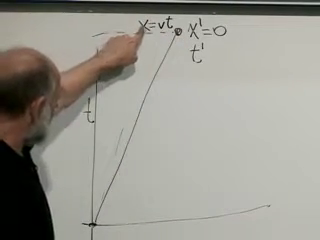
\includegraphics[width=0.72\textwidth]{lecture_04_figure_03.png}
\caption{El origen móvil: $x=vt$, $x'=0$ y el eje $t'$ son tres descripciones de la misma línea de universo.}
\lectureframe{00:48:18}
\end{figure}

Apliquemos el intervalo invariante entre el origen común y un punto posterior de esa línea de universo:
\begin{align}
t'^2-x'^2&=t^2-x^2,\\
t'^2&=t^2-v^2t^2,\\
t'&=t\sqrt{1-v^2}.
\label{eq:l4-time-dilation-natural}
\end{align}
Al restituir $c$,
\begin{equation}
\Delta\tau=\Delta t\sqrt{1-\frac{v^2}{c^2}}
=\frac{\Delta t}{\gamma},
\qquad
\gamma=\frac{1}{\sqrt{1-v^2/c^2}}.
\label{eq:l4-time-dilation}
\end{equation}

\begin{figure}[H]
\centering
\includegraphics[width=0.73\textwidth]{lecture_04_figure_09.png}
\caption{El resultado de la dilatación temporal en la pizarra: el reloj móvil acumula $t'=t\sqrt{1-v^2}$ en unidades con $c=1$.}
\lectureframe{00:50:45}
\end{figure}

El observador en reposo dice que el reloj móvil marcha más despacio. La reciprocidad exige que el observador móvil diga lo mismo de los relojes en reposo. No hay contradicción, porque las dos descripciones comparan pares distintos de sucesos distantes.

En efecto, un valor constante de $t'$ en la ec.~\eqref{eq:l4-lorentz-natural} satisface
\begin{equation}
t-vx=\text{constant}.
\label{eq:l4-simultaneity}
\end{equation}
Las líneas de simultaneidad del observador móvil están inclinadas respecto de las líneas horizontales $t=\text{constant}$. Cada observador considera simultáneas colecciones distintas de lecturas de relojes distantes. Si se tiene presente esta diferencia, la desaceleración recíproca de los relojes resulta coherente.

\begin{figure}[H]
\centering
\begin{tikzpicture}[x=1cm,y=1cm]
\draw[->] (0,0) -- (0,4.2) node[above] {$t$};
\draw[->] (0,0) -- (5.2,0) node[right] {$x$};
\draw[thick,->] (0,0) -- (2.4,3.8) node[above] {$x'=0$};
\draw[dashed] (0,2.8) -- (4.8,2.8)
  node[right] {$t=\mathrm{const}$};
\draw[thick] (0.15,1.05) -- (4.7,2.35)
  node[right] {$t'=\mathrm{const}$};
\draw[thick] (3.4,0) -- (3.4,3.8);
\fill (3.4,2.8) circle (0.045);
\fill (3.4,1.98) circle (0.045);
\end{tikzpicture}
\caption{La dilatación temporal recíproca compara lecturas de relojes en distintas superficies de simultaneidad.}
\end{figure}

\section{Las trayectorias de los gemelos}

Dos gemelos parten del mismo suceso. Uno permanece en $x=0$. El otro viaja hacia el exterior a velocidad $v$, invierte el sentido y regresa a la misma velocidad. Cuando se reúnen, comparan todos los procesos físicos que pueden servir como reloj: los relojes de pulsera, los latidos, el metabolismo o el envejecimiento mismo.

Supongamos que cada mitad del viaje dura un tiempo coordenado $T$ en el sistema del gemelo que se queda en casa. Su tiempo propio es
\begin{equation}
\tau_{\mathrm{home}}=2T.
\end{equation}
El suceso de retorno tiene coordenadas $(vT,T)$. Por tanto, el primer tramo del viaje aporta
\begin{align}
\tau_{\mathrm{leg}}
&=\sqrt{T^2-v^2T^2}
=T\sqrt{1-v^2}.
\end{align}
El tramo de regreso aporta la misma cantidad, de modo que
\begin{equation}
\tau_{\mathrm{travel}}=2T\sqrt{1-v^2}<2T.
\label{eq:l4-twin}
\end{equation}

\begin{figure}[H]
\centering
\includegraphics[width=0.73\textwidth]{lecture_04_figure_10.png}

\vspace{0.8em}

\begin{tikzpicture}[x=1.1cm,y=1cm]
\draw[->] (-0.2,0) -- (3.4,0) node[right] {$x$};
\draw[->] (0,-0.1) -- (0,4.4) node[above] {$t$};
\draw[very thick] (0,0) -- (0,4);
\draw[very thick] (0,0) -- (2.2,2) -- (0,4);
\draw[dashed] (0,2) -- (2.2,2);
\node[left] at (0,2) {$T$};
\node[left] at (0,4) {$2T$};
\node[below right] at (1.1,1.0) {$v$};
\node[above right] at (1.1,3.0) {$-v$};
\end{tikzpicture}\caption{La línea de universo del gemelo que se queda en casa y los dos tramos del viajero. Sus tiempos propios son distintos porque siguen trayectorias diferentes por el espacio-tiempo.}
\lectureframe{00:59:35}
\end{figure}

La diferencia de edad no es contradictoria. La trayectoria del viajero incluye un giro y no está relacionada con la trayectoria recta del gemelo que se queda en casa mediante una única simetría de sistema inercial. En la geometría euclidiana ordinaria, la ruta recta y una ruta quebrada entre dos puntos también tienen longitudes distintas. La geometría de Minkowski invierte cuál de las dos trayectorias tiene el intervalo mayor, pero la comparación sigue siendo geométrica.

\section{Aceleración y reloj ideal}

\begin{classroomqa}\audiencequestion{En el giro la física cambia y el viajero acelera. ¿Eso invalida el cálculo del reloj?
\lecturetimestamp{01:02:19}}\lecturerresponse{La aceleración es real y ayuda a identificar la asimetría; no se debe descartar con argumentos. La esquina pronunciada es solo una idealización gráfica y puede redondearse para representar un giro de duración finita. La hipótesis física adicional es que un reloj suficientemente pequeño y bien construido no se ve afectado por una aceleración moderada y sigue registrando el tiempo propio. Un reloj grande o frágil puede deformarse o romperse, pero eso es un defecto del mecanismo, no del intervalo del espacio-tiempo.}
\end{classroomqa}

Esta hipótesis del reloj ideal no se deduce únicamente de la transformación de Lorentz. Se pone a prueba observando el comportamiento de mecanismos de reloj reales. Un átomo constituye una aproximación mucho mejor que un reloj de cientos de millas de tamaño, porque es más difícil deformar su mecanismo compacto con la aceleración o la gravedad. Mencionar la relatividad general no eliminaría este problema físico: aún habría que saber cómo responde el mecanismo elegido a su entorno.

\begin{classroomqa}\audiencequestion{¿Puede reducirse una trayectoria acelerada a intervalos cortos en los que siga siendo válido el análisis inercial?
\lecturetimestamp{01:09:08}}\lecturerresponse{Sí. Dividamos la curva en segmentos cortos, casi rectos, calculemos el tiempo propio de cada segmento y sumemos los resultados. Es el análogo espacio-temporal de hallar la longitud de una curva ordinaria a partir de muchos segmentos pequeños. En el límite continuo,
\[
\tau=\int \sqrt{1-\frac{v(t)^2}{c^2}}\,dt,
\]
para un movimiento en el espacio-tiempo plano descrito en un sistema de coordenadas inercial.}
\end{classroomqa}

\section{Lo que ven los gemelos}

Las lecturas finales de los relojes pueden determinarse operacionalmente enviando pulsos de luz. Marquemos intervalos de un segundo de tiempo propio en ambas líneas de universo y hagamos que cada gemelo emita un pulso en cada marca. Durante el tramo de ida, los pulsos recibidos del otro gemelo llegan cada vez más espaciados. Durante el regreso, llegan agrupados. Este es el efecto Doppler relativista representado directamente en el diagrama del espacio-tiempo.

\begin{figure}[H]
\centering
\includegraphics[width=0.73\textwidth]{lecture_04_figure_11.png}
\caption{Señales luminosas intercambiadas entre las líneas de universo del gemelo que se queda en casa y el viajero. Las llegadas espaciadas durante el tramo de ida y las llegadas comprimidas durante el de regreso dan cuenta de todos los pulsos emitidos.}
\lectureframe{01:12:55}
\end{figure}

No desaparece ninguna parte de la historia. Cada observador acaba recibiendo todos los pulsos emitidos por el otro, pero la tasa de recepción depende del movimiento relativo. El corrimiento al rojo durante la ida y el corrimiento al azul durante el regreso no tienen la misma duración para las dos trayectorias, por lo que el recuento de todos los pulsos recibidos concuerda con la comparación de los tiempos propios.

\begin{classroomqa}\audiencequestion{Si el viajero que regresa recibe luz con corrimiento al azul, ¿podría recoger más energía de la que emitió la fuente?
\lecturetimestamp{01:13:50}}\lecturerresponse{Para responder hay que conocer la definición relativista de energía y su dependencia del sistema de referencia, conceptos que aún no se han desarrollado. La pregunta es razonable, pero las coordenadas y el recuento de pulsos por sí solos no bastan para resolver el balance energético, sobre todo para un observador acelerado. Por tanto, conviene dejar la respuesta para más adelante en vez de adivinarla.}
\end{classroomqa}

\section{Una dirección espacial cerrada}

\begin{classroomqa}\audiencequestion{Supongamos que una dirección espacial es compacta. ¿Podría un gemelo moverse uniformemente a su alrededor, regresar al punto de partida y evitar por completo la aceleración? En ese caso, ¿qué distinguiría a los gemelos?
\lecturetimestamp{01:15:14}}\lecturerresponse{El espacio debe imaginarse intrínsecamente como un cilindro, no como una lámina curvada dentro de un espacio mayor; no hace falta aceleración radial. Sin embargo, el observador que regresa se encuentra con el hecho global de que los mismos lugares vuelven a aparecer. Eso indica una asimetría, pero para dar una respuesta completa hace falta tratar cuidadosamente la relatividad especial con la identificación espacial. La pregunta se deja abierta aquí en vez de responderla de manera improvisada.}
\end{classroomqa}

\begin{figure}[H]
\centering
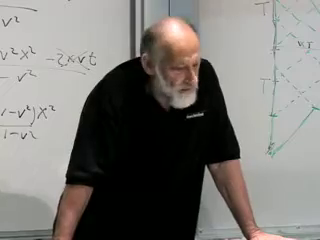
\includegraphics[width=0.72\textwidth]{lecture_04_figure_04.png}

\vspace{0.8em}

\begin{tikzpicture}[x=1cm,y=1cm]
\draw[thick] (0,0) ellipse (1.3 and 0.35);
\draw[thick] (-1.3,0) -- (-1.3,-3.1);
\draw[thick] (1.3,0) -- (1.3,-3.1);
\draw[thick] (0,-3.1) ellipse (1.3 and 0.35);
\draw[->,very thick] (0.0,0.38) arc (90:-210:1.38 and 0.42);
\node[right] at (1.65,-1.5) {compact spatial direction};
\end{tikzpicture}\caption{La cuestión del espacio compacto, tal como aparece en la pizarra, con un cilindro intrínseco bien definido. Se trata de una identificación global, no de un movimiento alrededor de un cilindro embebido en una dimensión radial adicional.}
\lectureframe{01:17:56}
\end{figure}

\section{La longitud se mide sobre una superficie de simultaneidad}

Ante un problema de relatividad especial, primero dibujemos el espacio-tiempo. Tomemos una regla de un metro en reposo en el sistema sin primas, con extremos en $x=0$ y $x=1$. A medida que pasa el tiempo, los dos extremos trazan líneas de universo verticales. La regla barre una cinta en el espacio-tiempo entre ellas.

El observador móvil debe medir ambos extremos en un mismo valor del tiempo móvil $t'$. Según la ec.~\eqref{eq:l4-simultaneity}, la superficie que pasa por el origen y cumple $t'=0$ satisface
\begin{equation}
t=vx
\end{equation}
en unidades de $c=1$. Esta superficie corta el extremo derecho $x=1$ en $t=v$.

\begin{figure}[H]
\centering
\includegraphics[width=0.73\textwidth]{lecture_04_figure_12.png}

\vspace{0.8em}

\begin{tikzpicture}[x=1.55cm,y=1.15cm]
\draw[->] (-0.5,0) -- (3.1,0) node[right] {$x$};
\draw[->] (0,0) -- (0,3.8) node[above] {$t$};
\draw[very thick,red] (0,0) -- (0,3.3);
\draw[very thick,red] (2.15,0) -- (2.15,3.3);
\fill[red!12] (0,0) rectangle (2.15,3.3);
\draw[very thick,green!50!black] (0,0) -- (1.2,3.1)
  node[above] {$x=vt$};
\draw[very thick,blue] (0,0) -- (2.15,1.15)
  node[right] {$t'=0$};
\fill (2.15,1.15) circle (0.045);
\node[right] at (2.22,1.35) {$(x,t)=(1,v)$};
\node[below] at (2.15,0) {$1$};
\end{tikzpicture}\caption{Una regla en reposo barre una cinta en el espacio-tiempo. La longitud medida por el observador móvil es la separación entre sus extremos sobre una superficie $t'=\mathrm{const}$.}
\lectureframe{01:24:20}
\end{figure}

La separación seleccionada entre los extremos es espacial, así que usamos la forma espacial positiva del invariante:
\begin{equation}
x'^2-t'^2=x^2-t^2.
\end{equation}
En el extremo elegido, $t'=0$, $x=1$ y $t=v$. Por tanto,
\begin{align}
x'^2&=1-v^2,\\
x'&=\sqrt{1-v^2}.
\end{align}
Así, en el sistema móvil, una longitud en reposo $L$ se mide como
\begin{equation}
L'=L\sqrt{1-v^2/c^2}=\frac{L}{\gamma}.
\label{eq:l4-length-contraction}
\end{equation}

\begin{figure}[H]
\centering
\includegraphics[width=0.76\textwidth]{lecture_04_figure_13.png}
\caption{La construcción completa de la contracción de la longitud y el resultado en la pizarra $x'=\sqrt{1-v^2}$ para una longitud en reposo unitaria.}
\lectureframe{01:28:10}
\end{figure}

También es cierta la afirmación recíproca: el observador del andén asigna una longitud menor a la regla longitudinal de un metro del tren. Una vez más, los dos observadores eligen sucesos simultáneos distintos para los extremos, de modo que la reciprocidad no es contradictoria.

\section{Preguntas finales}

\begin{classroomqa}\audiencequestion{¿Se propaga algo aparte de la luz a la velocidad de la luz? En particular, ¿qué ocurre con la gravedad?
\lecturetimestamp{01:29:29}}\lecturerresponse{La relatividad general predice ondas gravitacionales que se propagan a $c$. En la época de esta clase, las pruebas eran indirectas y provenían de sistemas como los púlsares binarios; todavía no se habían detectado ondas gravitacionales directamente.\editorialnote{La situación experimental cambió después de esta clase de 2006. LIGO detectó directamente GW150914 en 2015, y la observación conjunta de GW170817 y su contraparte electromagnética en 2017 mostró que las velocidades de propagación de la gravedad y de la luz coinciden con una diferencia de apenas unas pocas partes en $10^{15}$. Véanse \url{https://ligo.org/detections/gw150914/} y \url{https://doi.org/10.1103/PhysRevLett.119.251302}.}}
\end{classroomqa}

\begin{classroomqa}\audiencequestion{¿Puede un astronauta recorrer una distancia de muchos años luz en un tiempo propio menor que la distancia expresada en años luz? ¿Significaría eso que viaja más rápido que la luz?
\lecturetimestamp{01:30:38}}\lecturerresponse{El tiempo propio del astronauta es $\sqrt{\Delta t^2-\Delta x^2}$, menor que el tiempo coordenado $\Delta t$. En el sistema inercial del astronauta, la distancia entre las estrellas se contrae por Lorentz. Las estrellas se mueven con velocidad $-v$, no más rápido que la luz; simplemente hay menos distancia contraída que recorrer.}
\end{classroomqa}

Si el astronauta parte del reposo y acelera, la descripción cambia al pasar por una sucesión de sistemas inerciales instantáneos. La distancia asignada a las estrellas puede cambiar durante esa transición. No se puede aplicar una única transformación de Lorentz fija a toda la historia acelerada, pero el tiempo propio total sigue obteniéndose al sumar las contribuciones a lo largo de la línea de universo. Lo mismo vale para un gemelo realista que despega, gira y desacelera, en vez de nacer a velocidad de crucero.

\begin{classroomqa}\audiencequestion{¿Estos enigmas se deben a tratar el tiempo como algo especial? ¿Debemos llamarlo una cuarta dimensión?
\lecturetimestamp{01:36:43}}\lecturerresponse{No hace falta empezar con el eslogan de que el tiempo es una cuarta dimensión. La propia transformación de Lorentz obliga a que el espacio y el tiempo se mezclen, mientras que el intervalo $t^2-x^2-y^2-z^2$ los trata como partes de una misma geometría, con un signo distinto para el tiempo y el espacio. A bajas velocidades, la mezcla se vuelve despreciable y vuelve la intuición newtoniana habitual. Sin embargo, a velocidades relativistas, no se puede considerar que el espacio y el tiempo estén fundamentalmente desacoplados.}
\end{classroomqa}

Por tanto, la dilatación temporal, la contracción de la longitud, la comparación entre los gemelos y la reducción del tiempo de viaje no son trucos separados. Todo se desprende de tres hábitos: identificar los sucesos que se comparan, dibujar su geometría en el espacio-tiempo y usar el intervalo invariante.
\chapter{Bolas de fuego, sistemas de referencia y cuadrivectores}

Comenzamos con una pregunta que quedó pendiente de la discusión sobre colisiones de alta energía. La colisión de dos núcleos pesados crea un objeto que cambia violentamente, no un agujero negro astronómico tranquilo. ¿Qué puede significar, entonces, describir la colisión mediante un horizonte? La respuesta pasa por una imagen pentadimensional de la materia fuertemente acoplada y por una serie de preguntas prácticas sobre los aceleradores, para volver finalmente a la geometría de la relatividad especial. Al final, la velocidad y el momento se habrán convertido en cuadrivectores, y la energía ocupará su lugar junto a las tres componentes del momento.

\section{Una bola de fuego en una quinta dimensión}

\begin{classroomqa}\audiencequestion{El objeto producido en la colisión es inestable y cambia de forma. ¿Cómo se puede llamar agujero negro a un objeto tan complicado?}\lecturerresponse{Imaginemos una quinta dirección espacial que se extiende entre un suelo y un techo. La gravedad en esa dirección atrae las excitaciones hacia el suelo. La colisión deposita allí una masa de energía caliente; esta se expande y cambia de forma, pero aun así puede tener horizonte, temperatura y entropía.}\end{classroomqa}

Imaginemos partículas o, de forma más gráfica, pequeñas cuerdas que se mueven en este mundo pentadimensional. Las excitaciones que caen hacia el suelo aparecen en cuatro dimensiones como hadrones: protones, neutrones, mesones y otros objetos compuestos extendidos. Las excitaciones situadas cerca del techo parecen más elementales. Por tanto, la posición vertical es una forma geométrica de codificar la escala: el suelo representa el régimen hadrónico de grandes distancias, mientras que el techo representa los grados de libertad de distancias cortas.

Cuando chocan dos hadrones, dos objetos cerca del suelo se golpean y producen una gran salpicadura de energía. El resultado no es un cuerpo rígido. Es una masa caliente con horizonte, una especie de charco en el campo gravitatorio pentadimensional. No es un agujero negro astronómico en el espacio ordinario de cuatro dimensiones ni un agujero negro a escala de Planck situado junto al techo. Es la descripción gravitatoria de la bola de fuego fuertemente interactuante cerca del suelo.

A alta energía, los núcleos incidentes se contraen por Lorentz hasta convertirse en panqueques delgados. Chocan, depositan su energía en una región pequeña y producen un fluido que se expande hacia el equilibrio. Su baja viscosidad fue una de las características sorprendentes del plasma de quarks--gluones. En la descripción pentadimensional, la misma evolución es la relajación de un horizonte distorsionado.

\begin{figure}[H]\centering
\includegraphics[width=0.82\textwidth]{lecture_05_figure_01.png}\caption{La imagen del suelo y el techo para la quinta dimensión. Tras la colisión, la masa central con horizonte se expande a lo largo del suelo.}\lectureframe{00:04:22}\end{figure}

Un horizonte no dura para siempre. La radiación de Hawking se lleva energía y, en la descripción tetradimensional, esa radiación es la lluvia de hadrones ordinarios que emerge de la colisión. En este lenguaje, los miles de trazas de un suceso registrado por un detector son las partículas que se desprendieron por evaporación del agujero negro dual.

\subsection{¿Es real la dimensión extra?}

\begin{classroomqa}\audiencequestion{¿Es la quinta dimensión una dimensión espacial? ¿La línea dibujada entre el suelo y el techo se extiende literalmente en esa dirección?}\lecturerresponse{Sí. Es espacial, y la superficie dibujada en esa geometría pentadimensional es un horizonte. Si se llama ``real'' a esa dirección adicional o se la considera una descripción matemática equivalente es una cuestión más profunda.}\end{classroomqa}

La afirmación útil no es que la gravedad sustituya a la cromodinámica cuántica. Más bien, dos lenguajes pueden describir la misma física. En el lenguaje tetradimensional hay una bola de fuego caliente de quarks y gluones, sin un campo gravitatorio ordinario. En el lenguaje pentadimensional hay gravedad y un horizonte. Si la correspondencia es correcta, un cálculo genuino de QCD y el cálculo gravitatorio dual deben concordar allí donde ambos puedan realizarse.

\begin{classroomqa}\audiencequestion{La QCD no tiene gravedad ni horizontes. ¿La imagen del agujero negro añade física nueva o se limita a redescribir la bola de fuego?}\lecturerresponse{En cuatro dimensiones es un plasma de quarks y gluones; en su versión pentadimensional tiene una descripción gravitatoria con un horizonte. La ventaja es de cálculo. La QCD fuertemente acoplada es extremadamente difícil de tratar, mientras que algunas propiedades del horizonte---en particular, la viscosidad---son relativamente fáciles de calcular.}\end{classroomqa}

No es necesario zanjar la distinción entre una ``dimensión real'' y una ``analogía matemática'' para que la descripción resulte útil. Una estructura adquiere una interpretación física cuando integra las demás variables en un conjunto de leyes más sencillo y coherente. Aun así, no conviene exagerar el alcance de la afirmación: las aplicaciones de la dualidad gauge/gravedad al plasma de quarks--gluones observado son modelos de dinámica fuertemente acoplada, no una demostración de que se conozca un dual gravitatorio exacto para la QCD del mundo real.\editorialnote{Esta precisión explicita el estado actual de la aplicación a la QCD; no altera el mecanismo pentadimensional desarrollado aquí.}

\section{Por qué colisionan haces en los aceleradores}

Las preguntas pasan ahora a cuestiones prácticas. ¿Por qué se usan dos haces en movimiento en vez de un solo haz y un blanco en reposo? ¿Por qué son tan grandes los aceleradores circulares? ¿Por qué se trata de forma distinta a los electrones y los protones? Todas estas preguntas se refieren a la energía relativista.

\begin{classroomqa}\audiencequestion{¿Por qué hacer colisionar dos haces en vez de lanzar un haz energético contra un blanco en reposo?}\lecturerresponse{Lo que crea partículas nuevas es la energía disponible en el sistema del centro de masas. Dos haces relativistas iguales y opuestos tienen momento neto nulo, de modo que prácticamente toda su energía queda disponible para la colisión. Con un blanco fijo, gran parte de la energía incidente debe permanecer como movimiento del centro de masas.}\end{classroomqa}

Para dos partículas ultrarrelativistas con momentos opuestos de magnitud \(p\), la estimación aproximada de la clase, en unidades \(c=1\), es
\begin{equation}
E_{\mathrm{cm}}^{\mathrm{collider}}\simeq 2p.
\end{equation}
La estimación correspondiente para un blanco fijo crece solo como la raíz cuadrada del momento del haz:
\begin{equation}
E_{\mathrm{cm}}^{\mathrm{fixed}}\sim \sqrt{mp}.
\end{equation}
Lo relevante es el escalamiento, no el factor numérico omitido: duplicar la energía del haz duplica la energía del colisionador, pero solo aumenta en un factor raíz cuadrada la energía del centro de masas en el caso del blanco fijo.

El cálculo con invariantes permite precisar la comparación. Si \(P_1\) y \(P_2\) son los cuadrimomentos incidentes, entonces
\begin{equation}
s=(P_1+P_2)^2,
\qquad E_{\mathrm{cm}}=\sqrt{s}.
\end{equation}
Para dos haces iguales que se propagan en sentidos opuestos, cada uno con energía \(E\), los momentos espaciales se cancelan y \(\sqrt{s}=2E\). Para un proyectil de energía \(E\gg m\) que choca contra un blanco en reposo de la misma masa,
\begin{equation}
s=2m^2+2mE,
\qquad
\sqrt{s}\simeq \sqrt{2mE}
\qquad (c=1).
\end{equation}
Esta breve derivación mediante invariantes proporciona el factor omitido en la estimación oral.\editorialnote{Incluimos la derivación para que se pueda reproducir el argumento de escalamiento de la clase.}

\begin{classroomqa}\audiencequestion{¿Hay una razón fundamental por la que un acelerador circular tenga que ser tan grande? ¿No podría el mismo haz circular más veces por una máquina más pequeña?}\lecturerresponse{Los campos y los materiales imponen límites. Una partícula gana una cantidad finita de energía por metro, así que una máquina de mayor energía necesita una longitud efectiva de aceleración mayor. Además, una trayectoria circular cerrada exige más aceleración transversal y una carga acelerada emite radiación. Si el anillo es demasiado pequeño, el haz pierde energía por radiación tan rápido como la máquina se la suministra.}\end{classroomqa}

La relación para el curvado es aproximadamente
\begin{equation}
p=qBR,
\end{equation}
de modo que, para un campo magnético fijo \(B\), un momento mayor \(p\) exige un radio mayor \(R\). Las cavidades de radiofrecuencia realizan el trabajo que aumenta la energía del haz; los imanes lo curvan y lo enfocan. La idea general sigue siendo la expuesta en la pizarra: la intensidad del campo y las pérdidas por radiación impiden comprimir en un anillo pequeño un acelerador de energía arbitrariamente alta.

El movimiento circular implica aceleración incluso cuando la rapidez es constante, porque la velocidad cambia de dirección. Una carga acelerada emite radiación sincrotrón. Un acelerador lineal evita las pérdidas continuas por curvatura, aunque los breves impulsos de aceleración tampoco están literalmente libres de radiación. Las máquinas circulares aceptan el coste del curvado a cambio de reutilizar el mismo aparato en cada vuelta.

\begin{classroomqa}\audiencequestion{¿Por qué se asociaban los electrones con el acelerador lineal de SLAC, mientras que los colisionadores circulares de alta energía utilizan protones u otros hadrones?}\lecturerresponse{Los electrones son mucho más ligeros. A una energía alta dada, su factor de Lorentz es mucho mayor y la aceleración circular les hace emitir mucha más radiación. Los protones, más pesados, pueden dar vueltas repetidamente y ganar energía en cada paso antes de que las pérdidas por radiación sincrotrón se vuelvan prohibitivas.}\end{classroomqa}

A energía y radio del anillo fijos, la potencia radiada depende muy intensamente de la masa de la partícula:
\begin{equation}
P_{\mathrm{sync}}\propto \frac{E^4}{m^4R^2}.
\end{equation}
Por eso la diferencia entre electrones--y protones es mucho más marcada de lo que sugiere la expresión ``la partícula más ligera se mueve más rápido'': ambos haces pueden estar ya extremadamente cerca de \(c\), pero sus factores de Lorentz y sus pérdidas por radiación son muy diferentes.\editorialnote{La relación de curvatura y el escalamiento de la radiación sincrotrón precisan el argumento cualitativo de la clase sobre los aceleradores; no se desarrollaron en la pizarra.}

\begin{classroomqa}\audiencequestion{¿Por qué no acelerar también los hadrones en línea recta?}\lecturerresponse{Sí se puede. El problema es la longitud. En un anillo, la misma partícula pasa muchas veces por las estructuras de aceleración; una máquina lineal de hadrones equivalente tendría que ser enorme. El compromiso práctico es un anillo grande, lo bastante grande para que la radiación de los protones siga siendo tolerable.}\end{classroomqa}

Estas preguntas sobre aceleradores muestran con precisión por qué las reglas newtonianas no bastan. Volvamos ahora a la relatividad especial y construyamos el lenguaje que permite sistematizar estas comparaciones.

\section{El garaje y la limusina}

Consideremos un garaje de unos doce pies de largo y una limusina larga de unos veinte pies. El conductor acelera hasta que la limusina se contrae por Lorentz, con la esperanza de que quepa. En el sistema de referencia del garaje, la limusina en movimiento es más corta, así que parece posible. Sin embargo, en el sistema de referencia de la limusina, el garaje en movimiento es más corto, así que parece imposible. ¿Puede quedar toda la limusina dentro del garaje?

Abramos ambas puertas para que una colisión contra la pared no nos distraiga. Decir que la limusina está dentro significa que su parte delantera y su parte trasera están dentro \emph{simultáneamente}. Esa última palabra encierra todo el enigma.

Dibujemos un diagrama espaciotemporal con \(t\) en vertical y \(x\) en horizontal. Los rayos de luz forman el cono de luz de \(45^\circ\) en unidades \(c=1\). El garaje está en reposo, así que las líneas de universo de sus dos puertas son verticales. La parte delantera y la trasera de la limusina trazan dos líneas de universo inclinadas y paralelas. El eje \(t'\) del sistema en movimiento está inclinado hacia el cono de luz, y sus líneas de simultaneidad son paralelas al eje inclinado \(x'\).

\begin{figure}[H]\centering
\includegraphics[width=0.82\textwidth]{lecture_05_figure_02.png}\caption{Diagrama espaciotemporal completo del garaje--y la limusina. Las líneas verticales delimitan el garaje; las inclinadas trazan los dos extremos de la limusina. Los cortes horizontales e inclinados representan las distintas superficies de simultaneidad de los dos sistemas de referencia.}\lectureframe{00:31:05}\end{figure}

En el sistema de referencia del garaje, una línea horizontal puede cruzar las dos líneas de universo de la limusina entre las dos líneas de universo del garaje. En ese instante del garaje, la parte trasera ya ha entrado y la delantera aún no ha salido. La limusina contraída cabe por completo dentro.

En el sistema de referencia de la limusina, los sucesos simultáneos pertinentes están sobre una línea inclinada. Tracemos una línea así que pase por el suceso en que entra la parte trasera. Esta corta la línea de universo delantera después de que la parte delantera ya haya pasado la puerta del fondo. Según su propia noción de simultaneidad, la limusina nunca está completamente dentro. Ambas afirmaciones son verdaderas porque comparan pares distintos de sucesos.

\begin{classroomqa}\audiencequestion{¿Las dos líneas de universo verdes y el segmento horizontal entre ellas forman un paralelogramo? ¿Es ese segmento negro la longitud del vehículo?}\lecturerresponse{El segmento horizontal es la longitud contraída por Lorentz, porque sus extremos son simultáneos en el sistema del garaje. La longitud propia se obtiene con extremos simultáneos en el sistema de la limusina, sobre una línea paralela a \(x'\). Las dos mediciones usan cortes distintos del mismo par de líneas de universo.}\end{classroomqa}

Si \(L_0\) es la longitud propia, el corte horizontal en el sistema del garaje tiene longitud
\begin{equation}
L=\frac{L_0}{\gamma},
\qquad
\gamma=\frac{1}{\sqrt{1-v^2/c^2}}.
\end{equation}
La fórmula por sí sola no resuelve la paradoja. El diagrama sí, porque muestra qué sucesos se compararon. Siempre que un problema de relatividad parezca dar dos respuestas incompatibles, hay que buscar algún uso tácito de ``simultáneamente.''

\section{Cuatro coordenadas y dos posiciones de índice}

Para pasar de los enigmas a las leyes del movimiento, necesitamos una notación que tenga en cuenta la geometría. Agrupemos las coordenadas así:
\begin{equation}
(X^1,X^2,X^3,X^0)=(x,y,z,t),
\qquad X^\mu=(x,y,z,t),
\end{equation}
donde \(\mu\) recorre \(1,2,3,0\). En la página, este orden pone el tiempo al final, aunque su índice es \(0\), conforme a la convención usada en la pizarra.

\begin{classroomqa}\audiencequestion{¿Estamos tomando \(c=1\)? Si recuperamos las unidades ordinarias, ¿debería ser \(ct\) la coordenada temporal?}\lecturerresponse{Sí. Tomamos \(c=1\) al desarrollar la geometría y reponemos los factores de \(c\) cuando importan las dimensiones o el límite no relativista. Con las unidades de longitud convencionales, la coordenada temporal es \(ct\).}\end{classroomqa}

El mismo vector puede escribirse con un índice abajo. Con la convención de signos usada aquí,
\begin{equation}
X_\mu=(-x,-y,-z,t).
\end{equation}
Así, bajar un índice invierte los signos de las tres componentes espaciales y deja sin cambio la componente temporal. Por ejemplo:
\begin{equation}
X^\mu=(3,2,4,10)
\quad\Longrightarrow\quad
X_\mu=(-3,-2,-4,10).
\end{equation}
No se trata de dos puntos espaciotemporales, sino de dos formas de escribir las componentes de un mismo objeto geométrico.

\begin{classroomqa}\audiencequestion{¿Qué componentes son covariantes y cuáles contravariantes? ¿Se indican con superíndices o subíndices?}\lecturerresponse{Las componentes con índices arriba son contravariantes; las que tienen índices abajo son covariantes. Como regla mnemotécnica, se puede recordar ``co abajo, contra arriba.'' En física también se dice sencillamente «arriba» y «abajo».}\end{classroomqa}

La notación resulta útil en la contracción invariante
\begin{equation}
X_\mu X^\mu=t^2-x^2-y^2-z^2.
\label{eq:l5-interval}
\end{equation}
En forma diferencial,
\begin{equation}
d\tau^2=dt^2-dx^2-dy^2-dz^2
\qquad (c=1).
\label{eq:l5-proper-time}
\end{equation}
Para un movimiento de tipo temporal, \(d\tau\) es el tiempo que registra un reloj que se mueve a lo largo de la línea de universo.

Cuando un mismo índice aparece una vez arriba y otra abajo, se entiende que se suma sobre él. La convención de Einstein transforma
\begin{equation}
\sum_{\mu}X_\mu X^\mu
\end{equation}
en la expresión más breve de la ec.~\eqref{eq:l5-interval}. No se trata solo de economía tipográfica. Evita tener que volver a escribir a mano los signos alternantes de la geometría de Minkowski en cada ecuación.

\begin{classroomqa}\audiencequestion{¿Es \(\tau\) el símbolo estándar del tiempo propio?}\lecturerresponse{Sí. A veces también se usa el símbolo \(s\), pero \(\tau\) es una opción estándar para el tiempo propio.}\end{classroomqa}

\section{Las rotaciones como simetría sencilla}

Una transformación de Lorentz mezcla espacio y tiempo. Antes de estudiar esa matriz, consideremos la operación más familiar de rotar los ejes espaciales. Si el movimiento relativo apunta en una dirección arbitraria, podemos rotar los ejes hasta que esa dirección coincida con el nuevo eje \(x\) y aplicar entonces la transformación de Lorentz conocida. Por tanto, las rotaciones forman parte de la construcción; no son un desvío ornamental.

Para una rotación de ángulo \(\theta\) alrededor del eje \(z\),
\begin{align}
x'&=x\cos\theta+y\sin\theta,\nonumber\\
y'&=-x\sin\theta+y\cos\theta,\label{eq:l5-rotation}\\
z'&=z.\nonumber
\end{align}
Para \(\theta=0\), estas ecuaciones recuperan \(x'=x\) y \(y'=y\); para \(\theta=\pi/2\), intercambian los ejes con los signos esperados.

La transformación conserva la distancia euclídea. Si escribimos \(c_\theta=\cos\theta\) y \(s_\theta=\sin\theta\),
\begin{align}
x'^2+y'^2
&=(xc_\theta+ys_\theta)^2+(-xs_\theta+yc_\theta)^2\nonumber\\
&=x^2(c_\theta^2+s_\theta^2)
  +y^2(s_\theta^2+c_\theta^2)\nonumber\\
&\quad+2xyc_\theta s_\theta-2xyc_\theta s_\theta\nonumber\\
&=x^2+y^2.
\end{align}
Los términos cruzados se cancelan y \(c_\theta^2+s_\theta^2=1\). Como \(z'=z\), la longitud total \(x^2+y^2+z^2\) es invariante.

Las mismas ecuaciones se expresan en una sola ecuación matricial:
\begin{equation}
\begin{pmatrix}x'\\y'\\z'\end{pmatrix}
=
\underbrace{\begin{pmatrix}
\cos\theta&\sin\theta&0\\
-\sin\theta&\cos\theta&0\\
0&0&1
\end{pmatrix}}_{M}
\begin{pmatrix}x\\y\\z\end{pmatrix}.
\label{eq:l5-rotation-matrix}
\end{equation}
En notación de índices,
\begin{equation}
x'^i=M^i{}_{j}x^j,
\qquad i,j=1,2,3.
\end{equation}

\begin{figure}[H]\centering
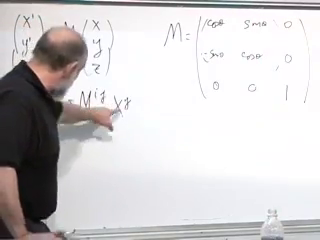
\includegraphics[width=0.82\textwidth]{lecture_05_figure_03.png}\caption{La rotación espacial expresada tanto mediante una ecuación matricial como en notación de índices.}\lectureframe{01:00:40}\end{figure}

\section{Matrices de Lorentz y composición de velocidades}

Para un movimiento a lo largo de \(x\), la transformación de Lorentz en unidades \(c=1\) es
\begin{align}
x'&=\gamma_v(x-vt), & y'&=y,\nonumber\\
z'&=z, & t'&=\gamma_v(t-vx),
\end{align}
donde
\begin{equation}
\gamma_v=\frac{1}{\sqrt{1-v^2}}.
\end{equation}
Con el orden de componentes \((x,y,z,t)\), queda
\begin{equation}
\begin{pmatrix}x'\\y'\\z'\\t'\end{pmatrix}
=
\begin{pmatrix}
\gamma_v&0&0&-\gamma_vv\\
0&1&0&0\\
0&0&1&0\\
-\gamma_vv&0&0&\gamma_v
\end{pmatrix}
\begin{pmatrix}x\\y\\z\\t\end{pmatrix}.
\label{eq:l5-lorentz-matrix}
\end{equation}

\begin{figure}[H]\centering
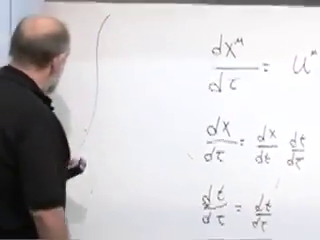
\includegraphics[width=0.82\textwidth]{lecture_05_figure_04.png}\caption{La matriz de Lorentz \(4\times4\). Solo se mezclan las componentes \(x\) y \(t\); \(y\) y \(z\) permanecen sin cambio.}\lectureframe{01:04:40}\end{figure}

La multiplicación de matrices permite responder ahora a una pregunta física. Supongamos que un observador se mueve con velocidad \(v\) respecto de nosotros y que un tercero se mueve con velocidad \(u\) respecto de ese observador, todos a lo largo del mismo eje. La cinemática newtoniana daría \(w=u+v\), lo que permitiría combinar dos velocidades de \(3c/4\) y obtener \(3c/2\). La relatividad debe dar una regla distinta.

La parte activa de la transformación de Lorentz es la matriz \(2\times2\)
\begin{equation}
B(v)=\gamma_v
\begin{pmatrix}1&-v\\-v&1\end{pmatrix}.
\end{equation}
Al componer las dos transformaciones se obtiene
\begin{align}
B(u)B(v)
&=\gamma_u\gamma_v
\begin{pmatrix}1&-u\\-u&1\end{pmatrix}
\begin{pmatrix}1&-v\\-v&1\end{pmatrix}\nonumber\\
&=\gamma_u\gamma_v
\begin{pmatrix}
1+uv&-(u+v)\\
-(u+v)&1+uv
\end{pmatrix}.
\label{eq:l5-composed-boost}
\end{align}
El cociente entre un elemento no diagonal y uno diagonal identifica la velocidad de la transformación resultante:
\begin{equation}
w=\frac{u+v}{1+uv}
\qquad(c=1).
\end{equation}
Al restablecer las dimensiones,
\begin{equation}
w=\frac{u+v}{1+uv/c^2}.
\label{eq:l5-velocity-addition}
\end{equation}

\begin{figure}[H]\centering
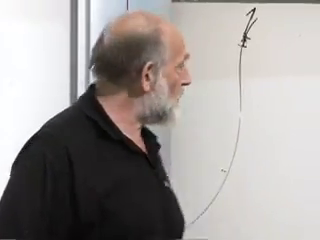
\includegraphics[width=0.82\textwidth]{lecture_05_figure_05.png}\caption{La matriz de la composición de dos transformaciones de Lorentz y la velocidad \(w=(u+v)/(1+uv)\) en unidades naturales.}\lectureframe{01:15:35}\end{figure}

Si \(u\) y \(v\) están ambas cerca de \(c\), el numerador se aproxima a \(2c\), mientras que el denominador se aproxima a \(2\); por tanto, \(w\) se aproxima a \(c\), no a \(2c\). En general, la ec.~\eqref{eq:l5-velocity-addition} transforma valores de entrada sublumínicos en un resultado sublumínico. La multiplicación de matrices ha incorporado automáticamente el límite de velocidad.

\section{Cuadrivectores y el fracaso de la velocidad ordinaria}

Un cuadrivector es cualquier objeto cuyas cuatro componentes se transforman bajo rotaciones y transformaciones de Lorentz del mismo modo que las coordenadas espaciotemporales. Si \(V^\mu\) es un cuadrivector, entonces, con nuestra convención de signos,
\begin{equation}
V_\mu=(-V^1,-V^2,-V^3,V^0),
\end{equation}
y su norma invariante es
\begin{equation}
V_\mu V^\mu=(V^0)^2-(V^1)^2-(V^2)^2-(V^3)^2.
\end{equation}
Para dos cuadrivectores \(V^\mu\) y \(W^\mu\), la contracción
\begin{equation}
W_\mu V^\mu
=W^0V^0-W^1V^1-W^2V^2-W^3V^3
\end{equation}
también es invariante. Las componentes cambian de un sistema de referencia a otro; la contracción no.

La velocidad ordinaria solo tiene tres componentes:
\begin{equation}
\mathbf v=\left(\frac{dx}{dt},\frac{dy}{dt},\frac{dz}{dt}\right).
\end{equation}
Añadir \(dt/dt=1\) no la convierte en un cuadrivector útil. La cuarta componente sería trivial y el objeto resultante no se transformaría linealmente bajo las transformaciones de Lorentz. El tiempo coordenado \(t\) cambia de un sistema de referencia a otro, así que derivar respecto de \(t\) arruina la ley de transformación deseada.

El tiempo propio resuelve el problema. A lo largo de una línea de universo, definamos
\begin{equation}
u^\mu=\frac{dX^\mu}{d\tau}.
\label{eq:l5-four-velocity}
\end{equation}
El diferencial \(dX^\mu\) es un cuadrivector y \(d\tau\) es invariante, de modo que su cociente también es un cuadrivector. El adjetivo ``propio'' alude al reloj que aparece en el denominador.

La regla de la cadena relaciona este objeto con la velocidad ordinaria:
\begin{equation}
\frac{dx}{d\tau}=\frac{dx}{dt}\frac{dt}{d\tau},
\end{equation}
y de igual modo para \(y\) y \(z\). De la ec.~\eqref{eq:l5-proper-time},
\begin{align}
\left(\frac{d\tau}{dt}\right)^2
&=1-\left(\frac{dx}{dt}\right)^2
    -\left(\frac{dy}{dt}\right)^2
    -\left(\frac{dz}{dt}\right)^2\nonumber\\
&=1-v^2
\qquad(c=1),
\end{align}
y, por tanto,
\begin{equation}
\frac{dt}{d\tau}=\gamma_v=\frac{1}{\sqrt{1-v^2}}.
\end{equation}
Las cuatro componentes son
\begin{equation}
u^i=\gamma_v v^i,
\qquad
u^0=\gamma_v
\qquad(c=1).
\label{eq:l5-four-velocity-components}
\end{equation}
A baja velocidad, \(u^i\simeq v^i\) y \(u^0\simeq1\). Cerca de la velocidad de la luz, \(\gamma_v\) crece sin límite y la velocidad propia difiere mucho de la velocidad ordinaria.

\begin{figure}[H]\centering
\includegraphics[width=0.82\textwidth]{lecture_05_figure_06.png}\caption{Las cuatro componentes de la velocidad propia expresadas en función de la velocidad ordinaria y del factor de Lorentz.}\lectureframe{01:34:40}\end{figure}

Al restablecer las unidades convencionales y usar \(X^0=ct\), se obtiene la forma estándar
\begin{equation}
U^\mu=(\gamma_v\mathbf v,\gamma_v c)
\end{equation}
con el orden espacial primero que se usa aquí. Su norma invariante es
\begin{equation}
U_\mu U^\mu=c^2.
\end{equation}
Así, todas las partículas masivas tienen una cuadrivelocidad de la misma magnitud invariante, aunque su velocidad espacial dependa del sistema de referencia.

\section{La tangente a una línea de universo}

La ec.~\eqref{eq:l5-four-velocity} tiene un modelo euclídeo familiar. A lo largo de una curva en el espacio tridimensional ordinario,
\begin{equation}
ds^2=dx^2+dy^2+dz^2.
\end{equation}
El desplazamiento diferencial \((dx,dy,dz)\) apunta a lo largo de la curva, pero no es un vector unitario. Al dividirlo por la longitud de arco se obtiene
\begin{equation}
\mathbf T=
\left(\frac{dx}{ds},\frac{dy}{ds},\frac{dz}{ds}\right),
\qquad
\mathbf T\cdot\mathbf T=1.
\end{equation}
La construcción relativista sigue la misma idea, pero usa el tiempo propio en lugar de la longitud de arco euclídea. El vector \(u^\mu=dX^\mu/d\tau\) es tangente a la línea de universo.

\begin{figure}[H]\centering
\includegraphics[width=0.82\textwidth]{lecture_05_figure_07.png}\caption{Construcción del vector tangente euclídeo: se divide el desplazamiento diferencial por el elemento de longitud de arco \(ds\). El tiempo propio cumple un papel análogo a lo largo de una línea de universo de tipo temporal.}\lectureframe{01:39:30}\end{figure}

\begin{classroomqa}\audiencequestion{Si \(c=1\), ¿son lo mismo el tiempo propio y la distancia propia?}\lecturerresponse{Tomar \(c=1\) pone el tiempo y la distancia en las mismas unidades; no elimina los signos menos de la geometría espaciotemporal. En la analogía euclídea, \(s\) es la distancia ordinaria medida a lo largo de una curva espacial. A lo largo de una línea de universo de tipo temporal, \(\tau\) es el tiempo transcurrido que mide un reloj. Las construcciones son análogas, pero las geometrías son distintas.}\end{classroomqa}

Al derivar una vez más se define la aceleración propia,
\begin{equation}
a^\mu=\frac{du^\mu}{d\tau}.
\end{equation}
Esta es la magnitud que debe sustituir a \(d^2\mathbf x/dt^2\) al formular la segunda ley de Newton de manera relativista. Como \(u_\mu u^\mu\) es constante,
\begin{equation}
\frac{d}{d\tau}(u_\mu u^\mu)=2u_\mu a^\mu=0,
\end{equation}
y, por tanto, la cuadraceleración es ortogonal a la cuadrivelocidad en la métrica de Minkowski.\editorialnote{La ortogonalidad se deduce directamente de la norma invariante y se incluye como siguiente consecuencia matemática de la definición.}

\section{Cuadrimomento y energía}

El momento es nuestro último ejemplo porque se conserva en colisiones y desintegraciones. La partícula tiene una masa intrínseca fija \(m\), llamada a menudo masa en reposo. No varía con la velocidad. El momento relativista es esa masa fija multiplicada por la cuadrivelocidad:
\begin{equation}
p^\mu=mu^\mu.
\label{eq:l5-four-momentum}
\end{equation}
En unidades \(c=1\),
\begin{equation}
p^i=\gamma_v m v^i,
\qquad
p^0=\gamma_v m.
\end{equation}
A velocidades bajas, \(\gamma_v\simeq1\), de modo que las componentes espaciales se reducen al momento newtoniano \(m\mathbf v\). A altas velocidades, crecen más rápidamente que \(m\mathbf v\).

La componente temporal es la energía. Con unidades convencionales y \(X^0=ct\),
\begin{equation}
P^\mu=(\mathbf p,E/c)
=(\gamma_v m\mathbf v,\gamma_v mc),
\end{equation}
y, por tanto,
\begin{equation}
E=\gamma_v mc^2
=mc^2\left(1-\frac{v^2}{c^2}\right)^{-1/2}.
\label{eq:l5-relativistic-energy}
\end{equation}

Para recuperar la mecánica ordinaria, tomemos
\(\epsilon=v^2/c^2\ll1\). El desarrollo binomial da
\begin{equation}
(1-\epsilon)^p=1-p\epsilon+O(\epsilon^2).
\end{equation}
Tomando \(p=-1/2\),
\begin{align}
E
&=mc^2\left(1-\frac{v^2}{c^2}\right)^{-1/2}\nonumber\\
&=mc^2\left[1+\frac12\frac{v^2}{c^2}
  +O\!\left(\frac{v^4}{c^4}\right)\right]\nonumber\\
&=mc^2+\frac12mv^2+O\!\left(\frac{mv^4}{c^2}\right).
\label{eq:l5-energy-expansion}
\end{align}

\begin{figure}[H]\centering
\includegraphics[width=0.82\textwidth]{lecture_05_figure_08.png}\caption{Desarrollo de la energía relativista a baja velocidad, que revela la energía en reposo y la energía cinética newtoniana.}\lectureframe{01:51:30}\end{figure}

El primer término, \(mc^2\), está presente incluso en reposo. En un problema newtoniano con un conjunto fijo de partículas y masas constantes, ese término suma la misma constante antes y después del movimiento, así que solo \(\tfrac12mv^2\) interviene en el balance habitual. La relatividad revela que esa constante descartada siempre fue energía física.

Por tanto, energía y momento no son leyes de conservación sin relación entre sí. Son las cuatro componentes de un único vector conservado. Una transformación de Lorentz los mezcla: lo que un observador llama energía contribuye en parte al momento de otro, y viceversa. Sin embargo, para un sistema aislado, el cuadrimomento total es el mismo antes y después de cualquier colisión o desintegración en todos los sistemas de referencia inerciales.

Este es el umbral de la mecánica relativista. Los siguientes pasos consisten en expresar la fuerza mediante la aceleración propia y comprender las ecuaciones de onda relativistas, en particular las que gobiernan el electromagnetismo y la luz.
\chapter{Leyes invariantes, cuatro-vectores y tensor de campo}

Comenzaremos con una ley que la naturaleza podría haber obedecido, pero no obedece. Su incumplimiento nos indicará cómo debe escribirse una ley física. Esta misma prueba nos lleva primero de las componentes de coordenadas a los vectores ordinarios, luego de estos a los cuatro-vectores y, por último, de los cuatro-vectores a los tensores. Al final, los campos eléctrico y magnético dejarán de ser objetos separados: juntos ocuparán las seis posiciones independientes de un único tensor antisimétrico.

Salvo que se indique lo contrario, usamos unidades en las que \(c=1\), ordenamos las componentes del espacio-tiempo como \((1,2,3,0)=(x,y,z,t)\) y usamos la signatura métrica \((-,-,-,+)\).

\section{Una posible ley con la simetría equivocada}

Fijemos permanentemente en el espacio un eje \(x\) y uno \(y\). Ahora establezcamos que dos partículas interactúan cuando sus coordenadas \(x\) coinciden. La interacción podría invertir su movimiento o hacer que partieran en nuevas direcciones; su dinámica detallada no importa. La condición que la desencadena es sencillamente \begin{equation}
  x_1-x_2=0,
\end{equation}, donde los subíndices identifican partículas, no componentes de coordenadas. Esta regla no encierra ninguna contradicción matemática. La pregunta es qué la hace físicamente poco plausible.

\begin{classroomqa}\audiencequestion{¿Viola la regla la homogeneidad del espacio?}\lecturerresponse{No. Trasladar el origen cambia ambas coordenadas en la misma cantidad y deja inalterado \(x_1-x_2\). La regla no especifica ningún lugar preferido. Su defecto es la isotropía: distingue una dirección preferida.}\end{classroomqa}

Giremos los ejes \(90^\circ\). Ahora llamamos \(y\) a la antigua dirección \(x\), de modo que los mismos sucesos físicos se describirían mediante la igualdad de las coordenadas \(y\). En un ángulo cualquiera, la condición incluiría una combinación lineal de \(x\) y \(y\). Por tanto, la forma de la ley depende de la orientación de la pizarra. Es invariante ante traslaciones, pero no ante rotaciones.

Solemos expresar las leyes físicas en su forma más sencilla usando coordenadas ortogonales. Se pueden usar coordenadas más generales, pero entonces la métrica y las fórmulas se vuelven menos sencillas. Dentro de la clase de marcos cartesianos ortogonales, ninguna orientación debe ser privilegiada.

La solución es inmediata. En dos dimensiones, exijamos que coincidan ambas coordenadas; en tres, las tres: \begin{equation}
  x_1=x_2,
  \qquad y_1=y_2,
  \qquad z_1=z_2.
\end{equation} Así, las partículas solo pueden interactuar cuando llegan al mismo punto, aunque se aproximen a él por líneas distintas.

\begin{classroomqa}\audiencequestion{¿También deben coincidir las coordenadas \(z\) y los tiempos?}\lecturerresponse{En el espacio tridimensional también deben coincidir las coordenadas \(z\). Por ahora dejamos de lado el tiempo; lo reincorporaremos en cuanto completemos el argumento espacial.}\end{classroomqa}

Sea \(\boldsymbol r_a\) la posición de la partícula \(a\). Las tres condiciones para las componentes se convierten en una ecuación vectorial: \begin{equation}
  \boldsymbol r_1-\boldsymbol r_2=\boldsymbol 0.
\end{equation} Una componente puede anularse en un marco rotado y no anularse en otro. El vector completo es distinto: si todas sus componentes son cero en un marco, también lo son en cualquier marco rotado. Del mismo modo, si dos vectores son iguales en un marco, siguen siéndolo después de transformar ambos.

\begin{figure}[H]\centering
\includegraphics[width=0.78\textwidth]{lecture_06_figure_01.png}\caption{Las tres igualdades de coordenadas que hacen que una colisión signifique coincidencia espacial, en vez de coincidencia a lo largo de un eje preferido.}\lectureframe{00:09:00}\end{figure}

Por eso son útiles las ecuaciones vectoriales. Sus componentes cambian, pero el objeto se transforma de manera coherente. Una ley expresada para el objeto completo puede conservar su forma cuando se rotan las coordenadas.

\section{Coincidencia en el espacio-tiempo}

Reemplacemos ahora el eje espacial vertical por el tiempo. Una regla newtoniana podría decir que dos cambios de movimiento solo ocurren en tiempos iguales. En la mecánica newtoniana, la simultaneidad es común a todos los observadores inerciales, así que tal regla es posible. En la relatividad especial, selecciona un marco preferido. Los sucesos simultáneos en un marco no tienen por qué serlo en otro.

Exigir solo la igualdad de las coordenadas espaciales no es mejor. Un desplazamiento espacio-temporal puede tener componentes espaciales nulas y una componente temporal distinta de cero: \begin{equation}
  \Delta X^\mu=(0,0,0,\Delta t),
\end{equation}, y una transformación de Lorentz mezcla \(\Delta t\) con una componente espacial. La afirmación local invariante es que los dos cambios de movimiento ocurren en el mismo suceso. Por tanto, una colisión simple exige \begin{equation}
  X_1^\mu=X_2^\mu,
  \qquad\text{or}\qquad
  X_1^\mu-X_2^\mu=0.
\end{equation} Las cuatro coordenadas coinciden: las partículas ocupan el mismo lugar en el mismo instante.

El ejemplo de la colisión da una regla general para formular la física. Podemos poner todo en un lado e igualar a cero un cuatro-vector completo, o igualar un cuatro-vector completo con otro. Igualar partes inconexas de un cuatro-vector no basta, por sí solo, para obtener una afirmación invariante de Lorentz.

\section{Transformaciones de Lorentz, rotaciones y notación matricial}

Un cuatro-vector es un objeto que se transforma como un desplazamiento espacio-temporal. Para que esta definición sea útil, recordemos primero las transformaciones de las propias coordenadas. Para una transformación de Lorentz con velocidad \(v\) en la dirección \(x\): \begin{align}
  x'&=\gamma(x-vt), & y'&=y, & z'&=z,
  & t'&=\gamma(t-vx),                                      \label{eq:l6-boost}
\end{align} donde \begin{equation}
  \gamma(v)=\frac{1}{\sqrt{1-v^2}}.
\end{equation}

\begin{classroomqa}\audiencequestion{¿En estas fórmulas se ha fijado la velocidad de la luz igual a uno?}\lecturerresponse{Sí. Para recuperar las unidades, tomemos \(X^0=ct\), reemplacemos \(1-v^2\) por \(1-v^2/c^2\) y restablezcamos los factores correspondientes de \(c\) en los términos mixtos de espacio--tiempo.}\end{classroomqa}

Una rotación alrededor del eje \(z\) mezcla \(x\) y \(y\), y deja sin cambios \(z\) y \(t\): \begin{equation}
\begin{pmatrix}
  x'\\ y'\\ z'\\ t'
\end{pmatrix}
=
\begin{pmatrix}
  \cos\theta & \sin\theta & 0 & 0\\
  -\sin\theta & \cos\theta & 0 & 0\\
  0 & 0 & 1 & 0\\
  0 & 0 & 0 & 1
\end{pmatrix}
\begin{pmatrix}
  x\\ y\\ z\\ t
\end{pmatrix}.
\end{equation} Conviene mostrar los ceros: indican explícitamente qué componentes no intervienen en una coordenada transformada determinada. En el mismo orden de componentes, la transformación de Lorentz de la ec.~\eqref{eq:l6-boost} es \begin{equation}
\begin{pmatrix}
  x'\\ y'\\ z'\\ t'
\end{pmatrix}
=
\begin{pmatrix}
  \gamma & 0 & 0 & -\gamma v\\
  0 & 1 & 0 & 0\\
  0 & 0 & 1 & 0\\
  -\gamma v & 0 & 0 & \gamma
\end{pmatrix}
\begin{pmatrix}
  x\\ y\\ z\\ t
\end{pmatrix}.
\end{equation}

Las rotaciones y las transformaciones de Lorentz se pueden componer mediante multiplicación de matrices. Para una transformación de Lorentz en una dirección que no esté alineada con el eje \(x\) original, se puede rotar esa dirección hasta alinearla con el eje \(x\), aplicar la transformación y rotar según haga falta. Los productos de estas matrices elementales generan transformaciones de Lorentz más generales.

\begin{classroomqa}\audiencequestion{¿Importa si primero se rota y luego se aplica una transformación de Lorentz, o si primero se aplica esta y luego se rota?}\lecturerresponse{Sí. Después de la primera operación, cambian los ejes sobre los que actúa la segunda. Los dos productos de matrices no tienen por qué coincidir, así que el orden de las operaciones importa.}\end{classroomqa}

Todas estas transformaciones lineales se pueden escribir de una sola vez como \begin{equation}
  X'^{\mu}=\Lambda^{\mu}{}_{\nu}X^{\nu}.                  \label{eq:l6-vector-transform}
\end{equation} El índice repetido \(\nu\) se suma sobre \(1,2,3,0\). No es más que la suma habitual de fila por columna en la multiplicación matricial, expresada en notación de índices.

\begin{figure}[H]\centering
\includegraphics[width=0.78\textwidth]{lecture_06_figure_02.png}\caption{La transformación de Lorentz con índices, encima de su forma con vectores columna.}\lectureframe{00:31:55}\end{figure}

La ec.~\eqref{eq:l6-vector-transform} también define un cuatro-vector contravariante general. Si \(A^\mu\) es uno de esos vectores, entonces \begin{equation}
  A'^{\mu}=\Lambda^{\mu}{}_{\nu}A^{\nu}.
\end{equation} Sus cuatro componentes no tienen por qué representar una posición. Lo que hace que el objeto sea un cuatro-vector es su ley de transformación.

\section{Escalares, la métrica y productos invariantes}

Antes de usar más cuatro-vectores, conviene volver a la noción más sencilla de escalar. Bajo rotaciones espaciales, la temperatura en un punto determinado es un escalar, al igual que la distancia entre dos puntos determinados. Cada uno es un solo número, independiente de la orientación de los ejes. Incluso se podría afirmar, deliberadamente y sin sentido físico profundo, que una distancia medida en centímetros es igual a la temperatura ambiente medida en grados Fahrenheit. La afirmación carece de profundidad física, pero, como ambos lados son escalares bajo rotaciones, su veracidad o falsedad no depende de cómo se giren los ejes.

Las componentes de un vector no son escalares. Por eso necesitamos una manera sistemática de combinarlas para obtener escalares. Escribamos un cuatro-vector contravariante general como \begin{equation}
  A^\mu=(A^1,A^2,A^3,A^0).
\end{equation} Las componentes covariantes describen el mismo objeto geométrico con un índice abajo. Con nuestra signatura se obtienen usando la métrica de Minkowski: \begin{equation}
  A_\mu=\eta_{\mu\nu}A^\nu,
  \qquad
  \eta_{\mu\nu}=
  \begin{pmatrix}
    -1&0&0&0\\
    0&-1&0&0\\
    0&0&-1&0\\
    0&0&0&1
  \end{pmatrix},                                          \label{eq:l6-metric}
\end{equation} de modo que \begin{equation}
  A_\mu=(-A^1,-A^2,-A^3,A^0).
\end{equation}

\begin{classroomqa}\audiencequestion{¿Hay dos índices y signos incoherentes en la pizarra?}\lecturerresponse{Sí. La componente espacial de la columna mostrada necesita el signo menos correspondiente, y las componentes a la derecha de la ecuación que baja los índices deben llevar índices superiores antes de multiplicarlas por \(\eta_{\mu\nu}\). La etiqueta temporal es \(0\), no \(4\).}\end{classroomqa}

\begin{figure}[H]\centering
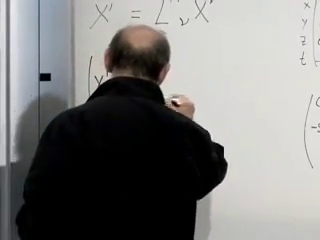
\includegraphics[width=0.8\textwidth]{lecture_06_figure_03.png}\caption{Componentes contravariantes y covariantes, la matriz métrica y el inicio de la contracción invariante.}\lectureframe{00:45:00}\end{figure}

Bajar índices no es un mero adorno. Incorpora los signos necesarios para obtener la norma invariante de Lorentz: \begin{align}
  A_\mu A^\mu
  &=-(A^1)^2-(A^2)^2-(A^3)^2+(A^0)^2,                    \label{eq:l6-norm}\\
  X_\mu X^\mu
  &=t^2-x^2-y^2-z^2.
\end{align} La segunda expresión es el intervalo espacio-temporal invariante desde el origen. Como \(A^\mu\) se transforma igual que \(X^\mu\), su contracción conserva la invariancia.

La notación también enseña una regla útil para llevar la cuenta. Un índice de suma aparece una vez arriba y otra abajo. Por ejemplo: \begin{equation}
  A_\mu A^\mu
  =\eta_{\mu\nu}A^\mu A^\nu.
\end{equation} Los nombres de los índices sumados, o mudos, se pueden cambiar sin alterar la cantidad.

\begin{classroomqa}\audiencequestion{¿Hay que considerar uno de estos vectores como una fila y el otro como una columna? ¿Importa el orden?}\lecturerresponse{Para el cálculo que hacemos, consideremos las cantidades con índices como componentes y dejemos que la métrica efectúe la contracción; no hace falta convertir la discusión en álgebra de operadores con vectores fila y columna. Son números ordinarios, así que el orden no importa. Los operadores que no conmutan requieren más cuidado, pero eso no es lo que tratamos aquí.}\end{classroomqa}

La misma construcción da el producto escalar entre dos cuatro-vectores distintos: \begin{equation}
  A\mathbin{\cdot}B=A_\mu B^\mu=A^\mu B_\mu.
\end{equation} Su invariancia se demuestra sin escribir explícitamente una matriz de Lorentz. Como \(A+B\) y \(A-B\) son cuatro-vectores, los cuadrados de sus normas son invariantes: \begin{align}
  (A+B)^2&=A^2+B^2+2A\mathbin{\cdot}B,\\
  (A-B)^2&=A^2+B^2-2A\mathbin{\cdot}B.
\end{align} Al restarlos se obtiene \begin{equation}
  (A+B)^2-(A-B)^2=4A\mathbin{\cdot}B,                    \label{eq:l6-polarization}
\end{equation}, por lo que \(A\mathbin{\cdot}B\) también es invariante. El factor cuatro se deduce directamente del desarrollo.\editorialnote{Este argumento de la pizarra da la identidad de polarización; escribir explícitamente el factor hace inequívoca la cancelación mencionada oralmente.}

\begin{figure}[H]\centering
\includegraphics[width=0.8\textwidth]{lecture_06_figure_04.png}\caption{Los dos cuadrados invariantes que se usan para aislar el producto escalar de cuatro-vectores distintos.}\lectureframe{00:52:20}\end{figure}

Las cantidades invariantes son ingredientes naturales de las leyes físicas: a diferencia de una componente aislada, conservan el mismo valor de un marco a otro.

\section{Velocidad propia y cuadrimomento}

Consideremos dos sucesos vecinos en la línea de universo de una partícula. Su separación es el cuatro-vector infinitesimal \begin{equation}
  dX^\mu=(dx,dy,dz,dt).
\end{equation} Para una línea de universo temporal, el tiempo propio se define mediante \begin{equation}
  d\tau^2=dX_\mu dX^\mu
  =dt^2-dx^2-dy^2-dz^2.                                  \label{eq:l6-proper-time}
\end{equation} La cuadrivelocidad propia es \begin{equation}
  U^\mu=\frac{dX^\mu}{d\tau}.                            \label{eq:l6-four-velocity}
\end{equation} Mide la tasa de cambio de la posición espacio-temporal con respecto al tiempo propio de la partícula, no con respecto al tiempo coordenado de un marco elegido.

Aunque \(U^\mu\) tiene cuatro componentes, solo tres son independientes. Al dividir la ec.~\eqref{eq:l6-proper-time} por \(d\tau^2\) se obtiene \begin{equation}
  U_\mu U^\mu=1.
\end{equation} Así, la cuadrivelocidad es un vector temporal unitario. La elección dirigida hacia el futuro fija el signo de su componente temporal.

\begin{classroomqa}\audiencequestion{Cuando las velocidades son mucho menores que \(c\), ¿se reduce la cuadrivelocidad a la velocidad ordinaria?}\lecturerresponse{Sus tres componentes espaciales se aproximan a la velocidad ordinaria, mientras que su componente temporal se aproxima a uno en unidades con \(c=1\). La relación se obtiene aplicando la regla de la cadena y calculando \(dt/d\tau\).}\end{classroomqa}

Para cada componente espacial, \begin{equation}
  U^i=\frac{dx^i}{d\tau}
     =\frac{dx^i}{dt}\frac{dt}{d\tau}
     =v^i\frac{dt}{d\tau}.
\end{equation} Dividamos la ec.~\eqref{eq:l6-proper-time} por \(dt^2\): \begin{equation}
  \left(\frac{d\tau}{dt}\right)^2
  =1-v_x^2-v_y^2-v_z^2
  =1-\boldsymbol v^2.
\end{equation} Por tanto, \begin{equation}
  \frac{dt}{d\tau}=\frac{1}{\sqrt{1-\boldsymbol v^2}}
  =\gamma(\lvert\boldsymbol v\rvert),
\end{equation} y \begin{equation}
  U^\mu=(\gamma v_x,\gamma v_y,\gamma v_z,\gamma).
                                                                  \label{eq:l6-u-components}
\end{equation}

\begin{figure}[H]\centering
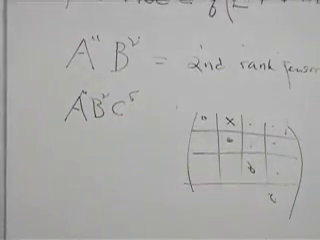
\includegraphics[width=0.8\textwidth]{lecture_06_figure_05.png}\caption{El cálculo con el tiempo propio que da \(dt/d\tau=\gamma\) y relaciona la velocidad propia con la velocidad ordinaria.}\lectureframe{01:02:00}\end{figure}

\begin{classroomqa}\audiencequestion{¿Significa \(dx^2/dt^2\) una segunda derivada, y al elevar al cuadrado un vector se obtienen términos cruzados?}\lecturerresponse{Aquí significa \((dx/dt)^2\), el cuadrado de una primera derivada. Además, \(\boldsymbol v^2\) significa el producto escalar euclídeo \(v_x^2+v_y^2+v_z^2\), no el cuadrado de la suma formal \(v_x+v_y+v_z\); no hay términos cruzados.}\end{classroomqa}

\begin{classroomqa}\audiencequestion{¿Es \(v\) en \(\gamma(v)\) la velocidad relativa de dos marcos de coordenadas o la velocidad de la partícula?}\lecturerresponse{Aquí es la velocidad de la partícula en el marco elegido. La función \(\gamma(v)=1/\sqrt{1-v^2}\) se puede evaluar para cualquier velocidad: en una transformación de Lorentz se evalúa para la velocidad relativa entre marcos; en la cuadrivelocidad, para la velocidad de la partícula.}\end{classroomqa}

Para \(v\ll1\), \(\gamma\simeq1\), así que las componentes espaciales de \(U^\mu\) se aproximan a \(\boldsymbol v\) y \(U^0\) se aproxima a uno. Cuando la velocidad ordinaria se aproxima a la velocidad de la luz, \(\gamma\) y todas las componentes no nulas de la cuadrivelocidad crecen sin límite.

\begin{classroomqa}\audiencequestion{¿No debería \(U^0\) tener unidades de velocidad, en lugar de ser cercano al número uno?}\lecturerresponse{Las unidades desaparecieron al fijar \(c\) igual a uno. Con \(X^0=ct\), se tiene \(U^\mu=(\gamma\boldsymbol v,\gamma c)\), así que la componente temporal se aproxima a \(c\) y \(U_\mu U^\mu=c^2\).}\end{classroomqa}

Para una partícula de masa en reposo \(m\), definamos el cuadrimomento mediante \begin{equation}
  P^\mu=mU^\mu.
\end{equation} En unidades naturales, \begin{equation}
  P^\mu=(\gamma m\boldsymbol v,\gamma m).
\end{equation} A bajas velocidades, las tres primeras componentes se aproximan al momento newtoniano \(m\boldsymbol v\). Al restablecer las unidades se obtiene \begin{equation}
  P^\mu=(\gamma m\boldsymbol v,E/c),
  \qquad E=\gamma mc^2,
\end{equation} y, por tanto, \begin{equation}
  E=mc^2+\frac{1}{2}m\boldsymbol v^2+O(mv^4/c^2).
\end{equation} La componente temporal es la energía en unidades con \(c=1\), o bien la energía dividida por \(c\) si se asignan unidades de momento a las cuatro componentes.

\begin{classroomqa}\audiencequestion{¿Es la velocidad ordinaria \(\boldsymbol v\), con una cuarta componente añadida, un cuatro-vector?}\lecturerresponse{No. La velocidad ordinaria tridimensional no se transforma como un cuatro-vector. El factor \(\gamma\) y la definición mediante el tiempo propio son esenciales; el cuatro-vector es \(U^\mu\), no \(\boldsymbol v\).}\end{classroomqa}

\section{Por qué deben mezclarse los campos eléctrico y magnético}

Ahora nos tomaremos lo que se llamó unas breves vacaciones de la relatividad. Empecemos con la ecuación de movimiento anterior a Einstein y preguntémonos cómo hay que reorganizarla para que sea válida en todos los marcos inerciales. La aceleración ordinaria es la derivada temporal de la velocidad ordinaria. Su análogo tetradimensional es, naturalmente, \begin{equation}
  A^\mu=\frac{dU^\mu}{d\tau}.
\end{equation} A bajas velocidades, sus componentes espaciales se aproximan a la aceleración ordinaria. Dejaremos para más adelante la ecuación relativista completa; primero examinemos la antigua ley de fuerza.

Para una carga \(q\) en campos eléctrico y magnético: \begin{equation}
  \boldsymbol F=m\boldsymbol a
  =q\left(\boldsymbol E+\boldsymbol v\times\boldsymbol B\right).
                                                                  \label{eq:l6-lorentz-force}
\end{equation} El término eléctrico es independiente de la velocidad de la partícula, mientras que el término magnético no lo es.

\begin{figure}[H]\centering
\includegraphics[width=0.8\textwidth]{lecture_06_figure_06.png}\caption{La forma prerrelativista de la ley de fuerza de Lorentz que motiva la combinación de \(\boldsymbol E\) y \(\boldsymbol B\).}\lectureframe{01:18:20}\end{figure}

Supongamos que un observador no ve ningún campo eléctrico, pero sí un campo magnético y una carga en movimiento. La carga siente una fuerza magnética. Sin embargo, en el marco de reposo instantáneo de la carga, \(\boldsymbol v=0\), así que el término magnético de la ec.~\eqref{eq:l6-lorentz-force} se anula. La línea de universo física no se vuelve inercial por el mero hecho de cambiar las coordenadas; por tanto, la fuerza en el nuevo marco debe incluir una contribución eléctrica. Más precisamente, una aceleración de cuatro dimensiones no nula no puede transformarse en cero cambiando de marco inercial, aunque la aceleración tridimensional y sus componentes sí se transformen. \editorialnote{Esta afirmación sobre la aceleración de cuatro dimensiones es la forma invariante del argumento de clase y evita tratar la aceleración ordinaria tridimensional como si fuera invariante de marco.}

Por consiguiente, los campos eléctrico y magnético deben transformarse uno en otro. Juntos tienen seis componentes, así que no forman ni un escalar ni un cuatro-vector. Necesitamos un nuevo objeto que se transforme.

\section{Tensores: una transformación por índice}

Un escalar puede llamarse tensor de rango cero; no tiene índices. Un cuatro-vector es un tensor de rango uno: tiene un índice con cuatro valores posibles. El ejemplo más sencillo de rango dos es un producto: \begin{equation}
  A^\mu B^\nu.
\end{equation} Cada índice tiene cuatro valores, así que el objeto tiene \(4^2=16\) componentes, que se pueden representar como un arreglo \(4\times4\). Un producto de tres vectores, \begin{equation}
  A^\mu B^\nu C^\sigma,
\end{equation}, tiene \(4^3=64\) componentes y es un tensor de rango tres. Los rangos superiores siguen el mismo patrón. El nombre importa menos que la regla que define el objeto.

Si \begin{equation}
  A'^{\mu}=\Lambda^\mu{}_{\nu}A^\nu,
  \qquad
  B'^{\sigma}=\Lambda^\sigma{}_{\tau}B^\tau,
\end{equation}, entonces su producto se transforma como \begin{equation}
  A'^{\mu}B'^{\sigma}
  =\Lambda^\mu{}_{\nu}\Lambda^\sigma{}_{\tau}
   A^\nu B^\tau.
\end{equation}. Esto da la ley que define un tensor contravariante de rango dos: \begin{equation}
  T'^{\mu\sigma}
  =\Lambda^\mu{}_{\nu}\Lambda^\sigma{}_{\tau}T^{\nu\tau}.
                                                                  \label{eq:l6-tensor-transform}
\end{equation} Hay una matriz de Lorentz por cada índice. Los índices repetidos \(\nu\) y \(\tau\) se suman; los índices libres \(\mu\) y \(\sigma\) identifican la componente que se calcula en el marco primado.

\begin{figure}[H]\centering
\includegraphics[width=0.82\textwidth]{lecture_06_figure_07.png}\caption{La transformación de dos vectores y la ley de transformación resultante, con dos matrices, para un tensor de rango dos.}\lectureframe{01:27:15}\end{figure}

Un tensor no tiene por qué ser el producto de un solo par de vectores. Tanto \(A^\mu B^\nu\) como \(A^\nu B^\mu\) obedecen la ley de transformación de los tensores, al igual que su suma y cualquier suma como \begin{equation}
  A^\mu B^\nu+C^\mu D^\nu.
\end{equation} La definición es la ley de transformación, no una factorización particular. Un tensor de rango tres adquiere una tercera matriz de Lorentz, y así sucesivamente.

\section{Tensores simétricos y antisimétricos}

Dos clases de tensores de rango dos serán especialmente útiles. Un tensor simétrico satisface \begin{equation}
  T^{\mu\nu}=T^{\nu\mu},
\end{equation}, de modo que las entradas reflejadas respecto de la diagonal son iguales. Sus cuatro entradas diagonales y las seis entradas a un lado de la diagonal determinan las demás, lo que da \begin{equation}
  4+6=10
\end{equation} componentes independientes.

Un tensor antisimétrico satisface \begin{equation}
  T^{\mu\nu}=-T^{\nu\mu}.                                \label{eq:l6-antisymmetry}
\end{equation}. Al poner \(\mu=\nu\) en la ec.~\eqref{eq:l6-antisymmetry} se obtiene \(T^{\mu\mu}=-T^{\mu\mu}\), así que todas las entradas diagonales se anulan. Las seis entradas de una mitad triangular determinan las otras seis con el signo cambiado. Por tanto, hay exactamente seis componentes independientes.

\begin{figure}[H]\centering
\includegraphics[width=0.82\textwidth]{lecture_06_figure_08.png}\caption{Un arreglo antisimétrico \(4\times4\) completo: ceros en la diagonal y signos opuestos a ambos lados.}\lectureframe{01:34:25}\end{figure}

Ese recuento da la pista. Las tres componentes eléctricas y las tres magnéticas pueden reunirse en un único tensor antisimétrico de rango dos.

\section{El tensor electromagnético}

Ordenemos las etiquetas del espacio-tiempo en filas y columnas como \((1,2,3,0)=(x,y,z,t)\). La matriz escrita en la pizarra es \begin{equation}
  F_{\mu\nu}=
  \begin{pmatrix}
    0    & -B_3 & B_2  & E_1\\
    B_3  & 0    & -B_1 & E_2\\
    -B_2 & B_1  & 0    & E_3\\
    -E_1 & -E_2 & -E_3 & 0
  \end{pmatrix}.                                         \label{eq:l6-field-tensor}
\end{equation} Las posiciones puramente espaciales contienen el campo magnético; las que llevan un índice espacial y uno temporal contienen el campo eléctrico. La antisimetría determina las entradas del triángulo inferior una vez conocidas las del triángulo superior.

\begin{classroomqa}\audiencequestion{¿Son negativas todas las entradas magnéticas, y corresponden las etiquetas a \(x,y,z\)?}\lecturerresponse{Los signos del triángulo espacial superior alternan como se muestra: \(-B_3,+B_2,-B_1\). Las etiquetas \(1,2,3\) corresponden a \(x,y,z\), mientras que \(0\) indica el tiempo. La reflexión respecto de la diagonal invierte todos los signos.}\end{classroomqa}

\begin{figure}[H]\centering
\includegraphics[width=0.82\textwidth]{lecture_06_figure_09.png}\caption{El tensor electromagnético completo con el orden de componentes espaciales primero usado en la lección.}\lectureframe{01:41:05}\end{figure}

La notación convencional es \(F_{\mu\nu}\), en lugar de un \(T_{\mu\nu}\) genérico. El profesor conjetura que la letra podría referirse a Faraday, aunque dice explícitamente que desconoce la historia de esta notación. Aquí lo que importa es la antisimetría y sus seis componentes de campo, no esa conjetura sobre la letra.

\begin{classroomqa}\audiencequestion{¿Representa cada entrada de la matriz la intensidad de un campo en el plano de coordenadas indicado?}\lecturerresponse{Es una componente del tensor electromagnético. Las entradas que incluyen el tiempo son componentes eléctricas, y las entradas espaciales--espaciales codifican componentes magnéticas.}\end{classroomqa}

Dejemos aparte la fila y la columna que llevan el índice temporal. El bloque antisimétrico \(3\times3\) restante es magnético. Sus componentes independientes se pueden recordar cíclicamente: \begin{equation}
  F_{12}=-B_3,
  \qquad F_{23}=-B_1,
  \qquad F_{31}=-B_2.                                   \label{eq:l6-magnetic-cycle}
\end{equation} Partiendo de la primera relación, avancemos cada etiqueta según \(1\to2\to3\to1\). De manera equivalente: \begin{equation}
  F_{ij}=-\epsilon_{ijk}B_k,
\end{equation}, con \(\epsilon_{123}=+1\).\editorialnote{La fórmula de Levi--Civita es la forma estándar y compacta de la regla cíclica desarrollada explícitamente en la pizarra.}

\begin{figure}[H]\centering
\includegraphics[width=0.82\textwidth]{lecture_06_figure_10.png}\caption{Las componentes espaciales cíclicas que codifican el campo magnético en el tensor antisimétrico.}\lectureframe{01:46:20}\end{figure}

Las identificaciones del campo eléctrico son más directas: \begin{equation}
  E_1=F_{10},
  \qquad E_2=F_{20},
  \qquad E_3=F_{30}.
\end{equation}

Por consiguiente, el campo magnético tiene dos identidades útiles. En el espacio tridimensional, se puede asociar un vector axial de tres componentes con un tensor antisimétrico \(3\times3\). Sin embargo, en el espacio-tiempo es solo la parte espacial del tensor de seis componentes \(F_{\mu\nu}\). Esta asociación es propia de tres dimensiones: un tensor antisimétrico \(4\times4\) tiene seis componentes independientes y no se puede identificar con un cuatro-vector.\editorialnote{Bajo rotaciones propias, el campo magnético se comporta como un vector; bajo reflexiones, es más precisamente un vector axial o pseudovector.}

El propósito de esta construcción no es contar componentes por el mero hecho de contarlas. Como \(F_{\mu\nu}\) se transforma como un tensor, una transformación de Lorentz mezcla automáticamente sus componentes eléctricas y magnéticas. En la próxima lección se puede combinar con la cuadrivelocidad y la cuadraceleración para reemplazar la ec.~\eqref{eq:l6-lorentz-force} por una ecuación de movimiento covariante.

\section{Preguntas sobre Einstein y Minkowski}

Los minutos finales pasan del formalismo a la historia de cómo surgió. Las respuestas se ofrecen como recuerdos, no como una historia establecida; esa salvedad forma parte del intercambio.

\begin{classroomqa}\audiencequestion{¿Buscaba Einstein una formulación invariante de Lorentz por razones conceptuales, o lo impulsaron observaciones concretas?}\lecturerresponse{El principio de que las leyes de la naturaleza deben tener la misma forma en todos los marcos inerciales fue central en su razonamiento. También había pruebas experimentales relacionadas con la luz y la imposibilidad de detectar el movimiento a través de un éter, aunque el profesor expresa explícitamente sus dudas sobre qué resultados conocía Einstein o cuánto influyeron en él. La motivación conceptual era que las ecuaciones de Maxwell y la fuerza de Lorentz debían obedecer el principio de relatividad, lo que exige que los campos eléctricos, los campos magnéticos y las componentes de la velocidad se transformen conjuntamente.}\end{classroomqa}

La exposición de Einstein de 1905 no usaba la notación compacta de cuatro-vectores que empleamos aquí. Trabajaba componente por componente y escribía explícitamente los factores necesarios de \(\gamma\) y de la velocidad. Posteriormente, Minkowski organizó geométricamente la misma estructura como un espacio-tiempo tetradimensional.

\begin{classroomqa}\audiencequestion{¿Se resistió Einstein a la formulación del espacio-tiempo de Minkowski, y cuánto tardó Minkowski en proponerla?}\lecturerresponse{El recuerdo que se ofrece en clase es que Einstein no acogió inicialmente con agrado el lenguaje geométrico tetradimensional, pero pronto reconoció su valor. La fecha se da con cautela como aproximadamente dos años después del artículo de 1905, quizá en 1907; el profesor recalca que está recordando la historia, no estableciéndola.}\end{classroomqa}

\begin{classroomqa}\audiencequestion{¿Minkowski era matemático o físico, qué otras contribuciones hizo y recibió influencia de Lorentz o FitzGerald?}\lecturerresponse{No se afirma tener una respuesta segura. No se profundiza en la distinción entre matemático y físico; una corrección del público interrumpe un comentario general sobre otros trabajos de Minkowski, y las posibles influencias se dejan expresamente como inciertas. El punto firme para esta discusión es la decisiva organización de la relatividad que hizo Minkowski mediante la notación geométrica tetradimensional.}\end{classroomqa}

\begin{classroomqa}\audiencequestion{¿Estaban ya presentes en el trabajo de Einstein de 1905 las transformaciones que mezclan \(\boldsymbol E\) y \(\boldsymbol B\)?}\lecturerresponse{Sí, pero escritas componente por componente en vez de como una sola ecuación para el tensor de campo. En clase se las compara con las ecuaciones de Maxwell escritas por componentes: el contenido puede estar presente antes de que una notación compacta revele su estructura común. La contribución de Minkowski fue sistematizar esa estructura en el lenguaje del espacio-tiempo.}\end{classroomqa}

Eso nos devuelve al punto matemático por el que empezamos. Los componentes son indispensables para los cálculos, pero la ley se vuelve inteligible cuando se reconocen como partes de un único objeto que se transforma. La siguiente tarea consiste en usar \(F_{\mu\nu}\) para escribir la ecuación de movimiento de la partícula cargada de una forma que sea la misma en todos los sistemas inerciales.
\chapter{Partículas cargadas, transformaciones de los campos y ondas relativistas}

La vez pasada empezamos a preguntarnos cómo se mueve una partícula cargada en campos eléctricos y magnéticos cuando se imponen los principios de la relatividad. La conocida ley de la fuerza de Lorentz ya contiene la pista: su término magnético depende de la velocidad de la partícula, así que distintos observadores no pueden concordar por separado sobre qué es eléctrico y qué es magnético. Nuestra tarea consiste en formular la ley de modo que todos los observadores inerciales usen la misma ecuación, aunque los campos y la velocidad de la partícula cambien de un sistema de referencia a otro.

Salvo que se indique lo contrario, usamos unidades en las que \(c=1\) y la signatura métrica \((-,-,-,+)\). Ordenamos las componentes del espacio-tiempo con las tres componentes espaciales primero: \begin{equation}
  \mu=(1,2,3,0)=(x,y,z,t).
\end{equation} Los índices latinos \(m,n\) recorren únicamente las tres direcciones espaciales.

\section{Qué queda de la ley de fuerza de Newton}

En mecánica newtoniana, \begin{equation}
  \boldsymbol F=m\boldsymbol a
\end{equation} tiene la misma forma en todos los sistemas de referencia inerciales porque los observadores galileanos coinciden en la aceleración. También asignan la misma masa y la misma fuerza a la partícula. Cuando cambia la cinemática, no hay razón para esperar que esta relación particular entre la fuerza y la aceleración ordinaria se conserve sin modificaciones.

El electromagnetismo y la gravitación ya nos advierten que las extensiones relativistas no tienen por qué parecerse entre sí. Tanto la ley de Coulomb como la ley de gravitación de Newton son leyes de la inversa del cuadrado, pero la gravitación no puede incorporarse de manera natural a la relatividad especial sin un cambio más profundo en la geometría del espacio-tiempo. El electromagnetismo sí puede. De hecho, el magnetismo es en sí mismo un efecto relativista: al reponer los factores de \(c\), la fuerza magnética lleva un factor de velocidad dividido por \(c\), y desaparece en el límite formal \(c\to\infty\).

La parte perdurable de la ley de Newton es la afirmación de que la fuerza es la tasa de cambio del momento. Para una masa en reposo constante, \begin{equation}
  \boldsymbol F
  =m\frac{d\boldsymbol v}{dt}
  =\frac{d}{dt}(m\boldsymbol v)
  =\frac{d\boldsymbol p}{dt}.
\end{equation} La relatividad modificará la relación entre el momento y la velocidad, pero conservará esta manera de organizar la ecuación.

\begin{figure}[H]\centering
\includegraphics[width=0.64\textwidth]{lecture_07_figure_01.png}\caption{La fuerza, reescrita como \(d\boldsymbol p/dt\), mientras se coloca en la pizarra la parte eléctrica de la ley de Lorentz.}\lectureframe{00:08:20}\end{figure}

En unidades \(c=1\), la ley de la fuerza de Lorentz prerrelativista es \begin{equation}
  \frac{d\boldsymbol p}{dt}
  =q\bigl(\boldsymbol E+\boldsymbol v\times\boldsymbol B\bigr).
  \label{eq:lorentz-three}
\end{equation} Ambos campos pueden depender de la posición y del tiempo. El límite no relativista es ahora el límite \(v\ll 1\), no un límite en el que la constante numérica \(c=1\) cambie de algún modo. El término eléctrico de \eqref{eq:lorentz-three} ya es un vector ordinario. Para entender el término magnético en una forma que pueda trasladarse al espacio-tiempo, tenemos que volver a examinar el producto vectorial.

\section{El producto vectorial como tensor antisimétrico}

Consideremos dos vectores tridimensionales \(\boldsymbol A\) y \(\boldsymbol B\). Su producto exterior \begin{equation}
  T_{mn}=A_mB_n
\end{equation} es un tensor de rango dos con nueve componentes. En general, no tiene ninguna simetría. Al antisimetrizarlo se obtiene \begin{equation}
  K_{mn}=A_mB_n-A_nB_m,
  \qquad K_{mn}=-K_{nm}.
  \label{eq:antisym-product}
\end{equation} Sus elementos diagonales se anulan, mientras que cada elemento por debajo de la diagonal queda determinado por el elemento correspondiente por encima de ella. Por tanto, un tensor antisimétrico \(3\times3\) tiene solo tres componentes independientes.

Ese recuento sugiere algo, pero no basta por sí solo. Tres cantidades no se transforman automáticamente como un vector. Sin embargo, en tres dimensiones, las tres entradas independientes de \eqref{eq:antisym-product} pueden identificarse con las componentes del producto vectorial \(\boldsymbol C=\boldsymbol A\times\boldsymbol B\). La pizarra muestra primero una ubicación provisional de \(C_2\) en la posición superior derecha:

\begin{figure}[H]\centering
\includegraphics[width=0.75\textwidth]{lecture_07_figure_02.png}\caption{El producto antisimétrico, mientras se identifican sus tres entradas independientes con las componentes de \(\boldsymbol C\). La etiqueta superior derecha aún es provisional.}\lectureframe{00:17:33}\end{figure}

Al recorrer cíclicamente \(1\to2\to3\to1\) se obtienen las fórmulas para las componentes \begin{align}
  C_3 &= A_1B_2-A_2B_1, \\
  C_1 &= A_2B_3-A_3B_2, \\
  C_2 &= A_3B_1-A_1B_3.
  \label{eq:cross-components}
\end{align} La última línea muestra que la entrada superior derecha es \(-C_2\), no \(C_2\). La corrección forma parte del argumento; no es un detalle que haya que ocultar.

\begin{figure}[H]\centering
\includegraphics[width=0.62\textwidth]{lecture_07_figure_03.png}\caption{Las identidades cíclicas completas para las componentes, que fijan el signo provisional en la matriz antisimétrica.}\lectureframe{00:21:54}\end{figure}

La matriz resultante es \begin{equation}
  K_{mn}=
  \begin{pmatrix}
    0 & C_3 & -C_2 \\
    -C_3 & 0 & C_1 \\
    C_2 & -C_1 & 0
  \end{pmatrix}.
  \label{eq:cross-matrix}
\end{equation}

Esta notación tiene una geometría útil detrás. Una componente con índices \(1,2\) pertenece de manera natural al plano \(xy\) y se identifica con una componente vectorial a lo largo del eje perpendicular \(z\). El mismo objeto orientado puede describirse mediante un plano o mediante una flecha normal a ese plano. La descripción con una flecha es propia de tres dimensiones; en dimensiones superiores sigue existiendo un tensor antisimétrico de rango dos, pero ya no tiene el mismo número de componentes que un vector. Por tanto, la forma del producto vectorial que se generaliza es el tensor, no la flecha perpendicular.

De forma equivalente, una vez elegida una orientación, \begin{equation}
  C_k=\frac12\epsilon_{kmn}K_{mn}.
\end{equation} La necesidad de elegir una orientación es el origen de la regla de la mano derecha y de la distinción conocida entre vectores polares y axiales. \editorialnote{La fórmula de Levi--Civita y la terminología de vector axial son notaciones estándar para la geometría del plano y la normal que se desarrolla explícitamente en la clase.}

\section{El campo magnético en forma tensorial}

La misma descripción dual se aplica al campo magnético. Definimos su tensor espacial antisimétrico mediante \begin{equation}
  B_{mn}=
  \begin{pmatrix}
    0 & -B_3 & B_2 \\
    B_3 & 0 & -B_1 \\
    -B_2 & B_1 & 0
  \end{pmatrix}.
  \label{eq:magnetic-tensor}
\end{equation} El signo global adicional con respecto a \eqref{eq:cross-matrix} es una convención. Una vez elegida, hay que usarla de manera coherente; cambiar el signo de las tres componentes vectoriales describiría la misma identificación entre tensor y vector con la convención de orientación opuesta.

\begin{figure}[H]\centering
\includegraphics[width=0.72\textwidth]{lecture_07_figure_04.png}\caption{El campo magnético expresado tanto como matriz espacial antisimétrica como en función de sus tres componentes vectoriales.}\lectureframe{00:24:40}\end{figure}

Consideremos ahora la tercera componente del producto vectorial: \begin{align}
  (\boldsymbol v\times\boldsymbol B)_3
  &=v_1B_2-v_2B_1 \\
  &=v_1B_{13}+v_2B_{23}+v_3B_{33}.
\end{align} Podemos añadir el último término porque \(B_{33}=0\). Al recorrer cíclicamente la componente libre se obtiene la regla compacta \begin{equation}
  (\boldsymbol v\times\boldsymbol B)_m=v_nB_{nm},
  \label{eq:cross-contraction}
\end{equation} donde se suma el índice repetido \(n\). Por tanto, la fuerza magnética es \begin{equation}
  F_m^{(B)}=qv_nB_{nm}.
\end{equation}

\begin{figure}[H]\centering
\includegraphics[width=0.78\textwidth]{lecture_07_figure_05.png}\caption{La tercera componente de \(\boldsymbol v\times\boldsymbol B\) y su expresión general como contracción con \(B_{nm}\).}\lectureframe{00:28:30}\end{figure}

\begin{classroomqa}\audiencequestion{¿El índice libre \(m\) designa una componente magnética separada de la fuerza?}\lecturerresponse{No. Designa la componente espacial de la fuerza que se esté calculando. Para el argumento actual, simplemente hemos fijado el campo eléctrico en cero, y todos los índices corresponden únicamente a las direcciones espaciales.}\end{classroomqa}

La notación tensorial hace casi automática la propiedad de campo magnético de no realizar trabajo. Derivemos el cuadrado de la rapidez: \begin{align}
  \frac{d}{dt}(v_mv_m)
  &=2\dot v_m v_m \\
  &\propto 2(\boldsymbol v\times\boldsymbol B)_m v_m \\
  &=2v_nB_{nm}v_m.
  \label{eq:speed-derivative}
\end{align} Los términos con \(m=n\) se anulan porque la diagonal de \(B_{nm}\) es cero. Cada término no diagonal tiene otro término correspondiente con \(m\) y \(n\) intercambiados; ambos se cancelan porque \(v_nv_m\) es simétrico mientras que \(B_{nm}\) es antisimétrico. Por tanto, \begin{equation}
  \frac{d}{dt}(v_mv_m)=0.
\end{equation} Una fuerza puramente magnética curva una trayectoria sin cambiar la rapidez ni la energía cinética.

\begin{figure}[H]\centering
\includegraphics[width=0.68\textwidth]{lecture_07_figure_06.png}\caption{Los términos emparejados de \(v_nB_{nm}v_m\) se cancelan porque el tensor magnético cambia de signo al intercambiar sus índices.}\lectureframe{00:35:40}\end{figure}

Esta demostración es deliberadamente más elaborada que decir que un producto vectorial es perpendicular a su primer factor. Esta última afirmación es propia de la representación vectorial tridimensional. La contracción de un par simétrico con un tensor antisimétrico es el argumento que se mantendrá en cuatro dimensiones.

\begin{classroomqa}\audiencequestion{¿Es necesario que el campo magnético sea independiente del tiempo para que la rapidez permanezca constante?}\lecturerresponse{El álgebra anterior nunca deriva el campo y no exige que \(\partial_t\boldsymbol B=0\). Un término puramente magnético sigue sin realizar trabajo. Sin embargo, en electrodinámica, un campo magnético variable produce un campo eléctrico, y ese campo eléctrico puede cambiar la rapidez de la partícula.}\end{classroomqa}

\section{Por qué deben mezclarse los campos eléctrico y magnético}

La mezcla de \(\boldsymbol E\) y \(\boldsymbol B\) puede apreciarse antes de cualquier cálculo cuatridimensional. Consideremos un movimiento lento, de modo que sean válidas las afirmaciones newtonianas ordinarias sobre la aceleración. Supongamos que un campo magnético apunta a lo largo del eje \(y\) y que una partícula cargada se mueve a lo largo del eje \(x\). La fuerza magnética apunta a lo largo del eje \(z\): \begin{equation}
  \boldsymbol F=q\boldsymbol v\times\boldsymbol B.
\end{equation}

\begin{figure}[H]\centering
\includegraphics[width=0.62\textwidth]{lecture_07_figure_07.png}\caption{Esquema de la pizarra de una partícula que se mueve transversalmente a un campo magnético; se usan las tres direcciones para comparar las descripciones del laboratorio y del sistema comóvil.}\lectureframe{00:42:20}\end{figure}

La geometría puede dibujarse de nuevo sin la perspectiva del aula: \begin{figure}[H]\centering
\begin{tikzpicture}[scale=1.05,>=Stealth]
  \draw[->] (0,0) -- (3.8,0) node[right] {\(x\)};
  \draw[->] (0,0) -- (-1.9,2.4) node[above left] {\(y\)};
  \draw[->] (0,0) -- (0,3.1) node[above] {\(z\)};
  \draw[->,very thick] (0,0) -- (2.7,0)
    node[midway,below] {\(\boldsymbol v\)};
  \draw[->,very thick] (0,0) -- (-1.35,1.7)
    node[midway,above left] {\(\boldsymbol B\)};
  \draw[->,very thick] (0,0) -- (0,2.35)
    node[midway,right] {\(\boldsymbol F,\ \boldsymbol E'\)};
\end{tikzpicture}\caption{En el laboratorio, la fuerza en dirección \(z\) es magnética; en el sistema comóvil instantáneo, la misma fuerza debe ser eléctrica.}\end{figure}

Introduzcamos ahora un observador que se mueve con la partícula en ese instante. La velocidad de la partícula en el nuevo sistema es cero, así que el término magnético \(q\boldsymbol v'\times\boldsymbol B'\) se anula. Sin embargo, en el límite de movimiento lento, ambos observadores deben coincidir en que la partícula tiene una aceleración en dirección \(z\). Si la ley de la fuerza de Lorentz tiene la misma forma en ambos sistemas, el observador comóvil debe atribuir la fuerza a un campo eléctrico \(\boldsymbol E'\) dirigido a lo largo de \(z\). Por tanto, un campo que era puramente magnético en el laboratorio no es puramente magnético en el sistema en movimiento.

Esta es la razón física para buscar un objeto cuyas componentes incluyan ambos campos. Un cambio de sistema de referencia no se limita a rotar \(\boldsymbol E\) entre sus propias tres componentes y \(\boldsymbol B\) entre las suyas; mezcla los dos conjuntos.

\section{El tensor del campo electromagnético}

En conjunto, los campos eléctrico y magnético tienen seis componentes. Un tensor antisimétrico cuatridimensional también tiene seis componentes independientes, ya que \begin{equation}
  \frac{4(4-1)}{2}=6.
\end{equation} Esto no significa que un tensor antisimétrico sea literalmente el único conjunto posible de seis cantidades: seis escalares, o un vector y dos escalares, también contendrían seis números. Es el objeto geométrico natural cuyas componentes pueden mezclarse de la manera requerida.

Para dejar explícita la convención de la pizarra, mostramos el tensor contravariante en el orden espacial primero \((1,2,3,0)\): \begin{equation}
  F^{\mu\nu}=
  \begin{pmatrix}
    0 & -B_3 & B_2 & E_1 \\
    B_3 & 0 & -B_1 & E_2 \\
    -B_2 & B_1 & 0 & E_3 \\
    -E_1 & -E_2 & -E_3 & 0
  \end{pmatrix}.
  \label{eq:l07-field-tensor}
\end{equation} El bloque superior izquierdo \(3\times3\) es precisamente el tensor magnético \eqref{eq:magnetic-tensor}; las componentes con un índice espacial y otro temporal contienen el campo eléctrico. La antisimetría determina las demás entradas.

\begin{figure}[H]\centering
\includegraphics[width=0.72\textwidth]{lecture_07_figure_08.png}\caption{El bloque espacial magnético y la columna espacio-tiempo eléctrica se ensamblan para formar el tensor del campo cuatridimensional.}\lectureframe{00:46:35}\end{figure}

\begin{classroomqa}\audiencequestion{¿Cuándo deben llevar estas componentes del campo índices superiores en vez de inferiores?}\lecturerresponse{Cuando solo aparecen las etiquetas espaciales, en la pizarra a veces se omite la distinción al identificar los campos de Maxwell--Faraday conocidos. En un cálculo covariante hay que restablecerla: subir o bajar un índice espacial cambia un signo con la convención métrica elegida.}\end{classroomqa}

Lo que es invariante no es una disposición concreta de signos en la pizarra, sino el tensor antisimétrico del espacio-tiempo junto con una convención coherente para la métrica y los índices. La notación \(F\) puede sugerir a Faraday, aunque la clase no afirma con seguridad esa atribución histórica. Einstein calculó la transformación de las componentes eléctricas y magnéticas en 1905; el lenguaje tensorial cuatridimensional compacto llegó después, con la formulación del espacio-tiempo asociada a Minkowski.

\section{Cuadrivelocidad y cuadrifuerza}

También hay que hacer covariante el lado de la ecuación correspondiente a la partícula. El tiempo propio \(\tau\) es invariante, así que al derivar el cuadrivector de posición con respecto a él se obtiene otro cuadrivector: \begin{equation}
  u^\mu=\frac{dx^\mu}{d\tau}
  =\gamma(v_x,v_y,v_z,1),
  \qquad
  \gamma=\frac{1}{\sqrt{1-v^2}}.
  \label{eq:four-velocity}
\end{equation} La última componente se deduce de \(dt/d\tau=\gamma\). El cuadrimomento es \begin{equation}
  p^\mu=mu^\mu,
\end{equation} cuya parte espacial es el momento relativista \(\boldsymbol p=m\gamma\boldsymbol v\).

\begin{figure}[H]\centering
\includegraphics[width=0.75\textwidth]{lecture_07_figure_09.png}\caption{Cuadrivelocidad, sus componentes, el factor de Lorentz y el cuadrimomento.}\lectureframe{00:50:30}\end{figure}

Como \(p^\mu\) es un cuadrivector y \(\tau\) es un escalar, el lado izquierdo relativista natural es \begin{equation}
  f^\mu\equiv\frac{dp^\mu}{d\tau}.
  \label{eq:four-force-def}
\end{equation} La cuadrifuerza no puede elegirse arbitrariamente. La cuadrivelocidad tiene norma fija, \begin{equation}
  u_\mu u^\mu=1.
\end{equation} Al derivar a lo largo de la línea de universo se obtiene \begin{align}
  0
  &=\frac{d}{d\tau}(u_\mu u^\mu) \\
  &=\frac{du_\mu}{d\tau}u^\mu
    +u_\mu\frac{du^\mu}{d\tau} \\
  &=2u_\mu\frac{du^\mu}{d\tau}.
\end{align} Para una masa constante, esto implica \begin{equation}
  f^\mu u_\mu=0.
  \label{eq:force-orthogonal}
\end{equation} Así, la cuadrifuerza es ortogonal a la cuadrivelocidad en el sentido de Minkowski. Es una restricción puramente cinemática que se deriva de la normalización de \(u^\mu\), no una propiedad especial del electromagnetismo.

\begin{figure}[H]\centering
\includegraphics[width=0.64\textwidth]{lecture_07_figure_10.png}\caption{La norma unidad de la cuadrivelocidad y la ortogonalidad resultante entre la cuadrifuerza y la cuadrivelocidad.}\lectureframe{00:56:50}\end{figure}

El cálculo magnético tridimensional ya nos ha dado el truco para satisfacer \eqref{eq:force-orthogonal}. Contraigamos un tensor antisimétrico con una copia de la velocidad: \begin{equation}
  \boxed{
  \frac{dp^\mu}{d\tau}=qF^{\mu\nu}u_\nu.}
  \label{eq:covariant-lorentz}
\end{equation} En efecto, \begin{equation}
  f^\mu u_\mu
  =qF^{\mu\nu}u_\nu u_\mu=0,
\end{equation} porque \(F^{\mu\nu}\) es antisimétrico y \(u_\nu u_\mu\) es simétrico. Esta no es la única ley de fuerza relativista concebible, pero sí la más sencilla que es lineal tanto en el campo electromagnético como en la velocidad.

\begin{figure}[H]\centering
\includegraphics[width=0.72\textwidth]{lecture_07_figure_11.png}\caption{La ecuación covariante de la fuerza de Lorentz a la izquierda y su contracción nula con una segunda cuadrivelocidad a la derecha.}\lectureframe{01:00:00}\end{figure}

\section{Recuperación de la fuerza de Lorentz ordinaria}

Una ecuación de apariencia covariante aún debe reproducir la ley de fuerza conocida. Con la convención métrica indicada al principio, \begin{equation}
  u_\mu=\gamma(-v_x,-v_y,-v_z,1).
\end{equation} Para la componente \(x\), \eqref{eq:l07-field-tensor} y \eqref{eq:covariant-lorentz} dan \begin{align}
  \frac{dp^1}{d\tau}
  &=q\bigl(F^{12}u_2+F^{13}u_3+F^{10}u_0\bigr) \\
  &=q\gamma\bigl(B_3v_y-B_2v_z+E_1\bigr) \\
  &=q\gamma\bigl[\boldsymbol E+\boldsymbol v\times
    \boldsymbol B\bigr]_x.
  \label{eq:x-force}
\end{align} Las demás componentes espaciales se obtienen recorriendo cíclicamente los índices.

\begin{classroomqa}\audiencequestion{¿Dónde aparece el término \(qE_x\) en el desarrollo en componentes?}\lecturerresponse{Es el término \(qF^{10}u_0\). Una componente del tensor de campo con un índice espacial y otro temporal es una componente del campo eléctrico, y \(u_0=\gamma\).}\end{classroomqa}

El factor \(\gamma\) del lado derecho no es una fuerza adicional. Puesto que \begin{equation}
  \frac{dp^i}{d\tau}=\frac{dt}{d\tau}\frac{dp^i}{dt}
  =\gamma\frac{dp^i}{dt},
\end{equation}, se cancela en ambos lados de \eqref{eq:x-force}. Por tanto, la ecuación espacial exacta vuelve a ser \begin{equation}
  \frac{d\boldsymbol p}{dt}
  =q\bigl(\boldsymbol E+\boldsymbol v\times\boldsymbol B\bigr),
  \qquad
  \boldsymbol p=m\gamma\boldsymbol v.
  \label{eq:exact-three-force}
\end{equation} Se conserva la forma conocida, pero la relatividad está contenida en el momento.

\begin{figure}[H]\centering
\includegraphics[width=0.75\textwidth]{lecture_07_figure_12.png}\caption{La ley de Lorentz tridimensional se recupera tras eliminar el factor común de tiempo propio; el momento conserva su factor de \(\gamma\).}\lectureframe{01:06:30}\end{figure}

La componente temporal contiene la afirmación correspondiente sobre la energía, \begin{equation}
  \frac{dp^0}{dt}=q\boldsymbol E\cdot\boldsymbol v,
\end{equation} así que un campo magnético no realiza trabajo, mientras que un campo eléctrico puede cambiar la energía de la partícula. \editorialnote{La comprobación de la componente temporal acompaña directamente el cálculo espacial de la clase; se incluye para mostrar la misma propiedad de ausencia de trabajo en notación cuatridimensional.}

\begin{classroomqa}\audiencequestion{¿Esta derivación es matemática o física?}\lecturerresponse{Es ambas cosas. El álgebra tensorial proporciona la forma compacta, pero intervino una cantidad considerable de física mediante el principio de que todos los sistemas inerciales obedecen las mismas leyes y mediante la suposición de que las ecuaciones de movimiento son de segundo orden. Una ley de segundo orden predice el futuro a partir de la posición y la velocidad; una ley de tercer orden requeriría la aceleración como dato inicial adicional. Es el experimento, no la notación, lo que nos indica qué tipo de ley sigue la naturaleza.}\end{classroomqa}

\section{Cómo se transforman los campos}

La ecuación \eqref{eq:covariant-lorentz} tiene la misma forma en todos los sistemas porque ambos lados son cuadrivectores. El propio tensor de campo se transforma con una matriz de Lorentz por cada índice: \begin{equation}
  F'^{\mu\nu}
  =\Lambda^\mu{}_{\rho}\Lambda^\nu{}_{\sigma}F^{\rho\sigma}.
  \label{eq:tensor-transform}
\end{equation} En la pizarra, esta regla se deriva transformando primero un producto sencillo \(A^\mu B^\nu\). Una vez conocida la regla para un producto de vectores, la linealidad permite obtener la regla para cualquier tensor de rango dos.

Para un impulso a lo largo del eje \(1\), las coordenadas se transforman como sigue: \begin{align}
  x'^1&=\gamma(x^1-vx^0), &
  x'^0&=\gamma(x^0-vx^1), \\
  x'^2&=x^2, & x'^3&=x^3.
\end{align} Apliquemos la misma transformación por separado a los dos índices del tensor. Para la componente paralela al impulso, la pizarra comienza con un producto: \begin{align}
  (A'^0B'^1)
  =\gamma^2\bigl(
     A^0B^1-vA^0B^0-vA^1B^1+v^2A^1B^0
   \bigr).
\end{align} Al sustituir cada producto por la componente tensorial correspondiente y usar después la antisimetría, \(F^{00}=F^{11}=0\) y \(F^{10}=-F^{01}\), se obtiene \begin{equation}
  F'^{01}
  =\gamma^2(1-v^2)F^{01}
  =F^{01}.
\end{equation} Así, la componente del campo eléctrico paralela al movimiento no cambia. La componente paralela del campo magnético se comporta de forma similar.

Las componentes transversales son diferentes. Siguiendo la convención de signos y de sistema primado que se usa en la pizarra, \begin{align}
  F'^{02}
  &=\gamma\bigl(F^{02}-vF^{12}\bigr), \\
  E'_2
  &=\gamma(E_2+vB_3).
  \label{eq:e-transform}
\end{align} Una componente transversal del campo eléctrico adquiere una parte de una componente magnética. Las demás leyes de transformación se obtienen con la misma regla de dos índices y quedan como ejercicio de la clase.

\begin{figure}[H]\centering
\includegraphics[width=0.76\textwidth]{lecture_07_figure_13.png}\caption{La transformación tensorial transversal, en el punto en que se observa que la componente \(E'_2\) contiene un término proporcional a \(vB_3\).}\lectureframe{01:23:40}\end{figure}

El signo de \eqref{eq:e-transform} depende de cuál sistema se declare que se mueve con \(+v\), así como de las convenciones para los índices y la métrica. Su contenido invariante no depende de ello: las componentes transversales eléctricas y magnéticas se mezclan, y la ecuación covariante de la fuerza sigue siendo válida después de la transformación.

\begin{classroomqa}\audiencequestion{En el caso de una corriente en un cable, ¿es posible moverse a alguna velocidad que haga desaparecer el campo magnético?}\lecturerresponse{Moverse con los electrones de conducción no basta, porque entonces las cargas positivas de la red se mueven en el nuevo sistema. Por tanto, un cable neutro por el que circula corriente es más sutil que un único cúmulo de carga en movimiento. Un campo puramente magnético no puede eliminarse por completo mediante una transformación. Si están presentes tanto el campo eléctrico como el magnético, sus componentes transformadas pueden cancelarse en circunstancias especiales; para una carga que se mueve uniformemente, el sistema en reposo de la carga es el sistema sencillo en el que desaparece su campo magnético.}\end{classroomqa}

La prueba invariante precisa usa \begin{equation}
  \boldsymbol B^2-\boldsymbol E^2,
  \qquad
  \boldsymbol E\cdot\boldsymbol B.
\end{equation} Solo puede existir un sistema en el que \(\boldsymbol B'=0\) para un campo dominado por el campo eléctrico que cumpla \(\boldsymbol E\cdot\boldsymbol B=0\); un campo que sea puramente magnético en un sistema está dominado por el campo magnético y no puede cumplir esa condición. \editorialnote{Estos criterios invariantes expresan con precisión la salvedad que se planteó en el aula; su derivación queda aplazada.}

\begin{classroomqa}\audiencequestion{¿El potencial escalar eléctrico y el potencial vectorial magnético forman un cuadrivector?}\lecturerresponse{Sí. Con signos que dependen de la convención, se combinan en el cuadripotencial \(A^\mu\). Las ecuaciones de Maxwell harán uso sistemático de ese objeto.}\end{classroomqa}

\section{Derivadas de los campos}

Dejamos ahora la trayectoria de una sola partícula y consideramos un campo en todo el espacio-tiempo. Sea \begin{equation}
  \phi=\phi(x^1,x^2,x^3,x^0)
\end{equation} un campo escalar. Sus cuatro derivadas forman las componentes covariantes de un cuadrivector: \begin{equation}
  \partial_\mu\phi
  \equiv\frac{\partial\phi}{\partial x^\mu}
  =\left(
    \frac{\partial\phi}{\partial x},
    \frac{\partial\phi}{\partial y},
    \frac{\partial\phi}{\partial z},
    \frac{\partial\phi}{\partial t}
  \right).
\end{equation} La regla de la cadena aplicada a la transformación de Lorentz de las coordenadas demuestra esta ley de transformación covariante. Al subir el índice se invierten los signos espaciales, pero el signo temporal permanece igual: \begin{equation}
  \partial^\mu\phi
  =\left(
    -\frac{\partial\phi}{\partial x},
    -\frac{\partial\phi}{\partial y},
    -\frac{\partial\phi}{\partial z},
    \frac{\partial\phi}{\partial t}
  \right).
\end{equation}

Cada derivación aporta un índice inferior. Así, \(\partial_\nu V^\mu\) es un tensor de rango dos con un índice superior y otro inferior, y al derivar un tensor se obtiene un objeto con un índice inferior adicional. Esta es la regla básica necesaria para escribir ecuaciones de campo sin elegir un sistema de referencia inercial privilegiado.

\section{La ecuación de onda escalar invariante}

Las ecuaciones de onda más sencillas contienen dos derivadas. Si la ecuación ha de tener la misma forma en todos los sistemas inerciales, su lado izquierdo debe ser un escalar. La contracción de los índices de las derivadas da la opción más sencilla: \begin{equation}
  \boxed{\partial^\mu\partial_\mu\phi=0.}
  \label{eq:wave-covariant}
\end{equation} Al desarrollar las componentes con la signatura actual, \begin{equation}
  \frac{\partial^2\phi}{\partial t^2}
  -\frac{\partial^2\phi}{\partial x^2}
  -\frac{\partial^2\phi}{\partial y^2}
  -\frac{\partial^2\phi}{\partial z^2}=0.
  \label{eq:wave-components}
\end{equation} La contracción en \eqref{eq:wave-covariant} hace manifiesta la invariancia de Lorentz; la ecuación \eqref{eq:wave-components} expresa lo mismo componente por componente.

\begin{figure}[H]\centering
\includegraphics[width=0.75\textwidth]{lecture_07_figure_14.png}\caption{La forma contraída de la ecuación de onda escalar y su desarrollo en componentes como derivada temporal menos derivadas espaciales.}\lectureframe{01:39:40}\end{figure}

\begin{classroomqa}\audiencequestion{¿El lado derecho de la ecuación de onda debe ser cero?}\lecturerresponse{No. Puede ser cualquier escalar compatible con el problema. Una constante multiplicada por \(\phi\), o una función escalar no lineal como una proporcional a \(\phi^2\), sigue preservando la covariancia. Cero da la ecuación de onda libre más sencilla.}\end{classroomqa}

El propósito de este ejemplo escalar es prepararnos. Las ecuaciones de Maxwell mezclan los campos eléctrico y magnético de manera más compleja, pero también pueden escribirse de modo que la invariancia de Lorentz quede manifiesta en la estructura de sus índices. Ese es el problema al que volveremos la próxima vez.
\chapter{Métrica, expansión y una primera cosmología}

Al final de la clase anterior habíamos llegado a una ecuación de ondas invariante de Lorentz y nos disponíamos a escribir las ecuaciones de Maxwell en forma espaciotemporal. Una pregunta del público nos da ahora una advertencia útil antes de pasar a la gravitación: ¿hasta qué punto puede la simetría determinar por sí sola una teoría física? La respuesta es tajante: mucho, pero no todo. La invariancia de Lorentz es un poderoso filtro para las leyes posibles. No sustituye los demás supuestos físicos ni los experimentos.

\section{Lo que la simetría no determina}

\begin{classroomqa}
\audiencequestion{Una vez que sabemos que los campos eléctrico y magnético se transforman conjuntamente bajo las transformaciones de Lorentz, ¿se deducen las ecuaciones de Maxwell solo de la relatividad?}
\lecturerresponse{No. La relatividad restringe la forma de las ecuaciones, pero para construirlas también se recurre a su linealidad, al bajo orden de sus derivadas, a la manera en que se transforman los campos y a la información experimental. Sin esos ingredientes adicionales, seguirían siendo posibles muchas ecuaciones de campo covariantes de Lorentz.}
\end{classroomqa}

El supuesto adicional más importante para esta introducción es la linealidad. Si \(A(x,t)\) es una solución de una ecuación de campo lineal, entonces \(\lambda A(x,t)\) también lo es para cualquier constante \(\lambda\). Si \(A\) y \(B\) son soluciones, entonces también lo es \begin{equation}
  C(x,t)=A(x,t)+B(x,t).
  \label{eq:superposition}
\end{equation}
Este es el principio de superposición. Dos ondas electromagnéticas sin fuentes pueden cruzarse y salir intactas. No chocan directamente como lo hacen los objetos materiales. Pueden interactuar indirectamente a través de la materia cargada, porque cada onda mueve las cargas y las cargas en movimiento emiten radiación; sin embargo, las propias ecuaciones de campo en el vacío son lineales.

\begin{figure}[H]
\centering
\includegraphics[width=0.64\textwidth]{lecture_08_figure_01.png}
\caption{Dos perfiles de onda en la pizarra durante la explicación de la superposición. Su suma vuelve a ser una onda sin fuentes admisible.}
\lectureframe{00:05:30}
\end{figure}

El oscilador armónico hace transparente el álgebra. Supongamos que \begin{equation}
  m\ddot x=-kx.
  \label{eq:linear-oscillator}
\end{equation}
Si \(x_1\) y \(x_2\) satisfacen \eqref{eq:linear-oscillator}, entonces \begin{equation}
  m(\ddot x_1+\ddot x_2)
  =-k(x_1+x_2),
\end{equation}
por lo que \(x_1+x_2\) es una solución. Sin embargo, si añadimos un término no lineal, \begin{equation}
  m\ddot x=-kx+p x^2,
  \label{eq:nonlinear-oscillator}
\end{equation}
la suma ya no funciona:
\begin{equation}
  (x_1+x_2)^2=x_1^2+x_2^2+2x_1x_2.
\end{equation}
El término cruzado \(2x_1x_2\) no tiene un término correspondiente en las dos ecuaciones por separado. Ahora los dos movimientos se influyen mutuamente.

\begin{figure}[H]
\centering
\includegraphics[width=0.73\textwidth]{lecture_08_figure_02.png}
\caption{Comparación entre las ecuaciones de los osciladores por separado y la ecuación para su suma. El término cuadrático deja al descubierto el término cruzado adicional que rompe la superposición.}
\lectureframe{00:10:10}
\end{figure}

Este ejemplo fija el punto metodológico que se mantendrá durante toda la exposición sobre cosmología. La simetría nos dice qué magnitudes pueden combinarse y qué ecuaciones son admisibles. La dinámica y la observación nos dicen cuál de las ecuaciones admisibles utiliza la naturaleza.

\section{El intervalo como geometría}

Dejamos ahora el electromagnetismo y tomamos un breve camino hacia la relatividad general y la cosmología. El objeto de partida es el intervalo entre sucesos vecinos. Etiquetemos un suceso con cuatro coordenadas \(x^\mu\) y un suceso cercano con \(x^\mu+dx^\mu\). En coordenadas cartesianas inerciales, con \(c=1\) y la convención \((+,-,-,-)\),
\begin{equation}
  d\tau^2
  =dt^2-dx^2-dy^2-dz^2
  =dx^\mu dx_\mu
  =\eta_{\mu\nu}\,dx^\mu dx^\nu.
  \label{eq:minkowski-interval}
\end{equation}
La cantidad invariante es \(d\tau^2\), no una diferencia de coordenadas particular. Las transformaciones de Lorentz cambian \(dt,dx,dy,dz\), pero conservan esta combinación cuadrática. Por tanto, la relatividad especial puede entenderse como la geometría del espaciotiempo de Minkowski.

\begin{figure}[H]
\centering
\includegraphics[width=0.72\textwidth]{lecture_08_figure_03.png}
\caption{El intervalo de Minkowski escrito sucesivamente en notación por componentes, con índices contraídos y con el tensor métrico.}
\lectureframe{00:14:50}
\end{figure}

La sencillez de \eqref{eq:minkowski-interval} depende de las coordenadas. Incluso un plano llano puede adquirir coeficientes poco familiares si lo etiquetamos de manera poco conveniente. Supongamos que \(x\) se mide en centímetros y \(y\) en metros. Para un desplazamiento físico,
\begin{equation}
  ds^2=dx^2+\left(\frac{dy}{100}\right)^2
      =dx^2+10^{-4}dy^2.
  \label{eq:mixed-units}
\end{equation}
El factor \(10^{-4}\) no dice nada sobre la curvatura. Solo convierte entre unidades.

\begin{figure}[H]
\centering
\includegraphics[width=0.59\textwidth]{lecture_08_figure_04.png}
\caption{Un plano llano descrito con centímetros en un eje y metros en el otro. Los coeficientes métricos desiguales codifican las unidades, no la curvatura.}
\lectureframe{00:20:10}
\end{figure}

Las coordenadas oblicuas añaden un término mixto. En dos dimensiones, la forma cuadrática local más general puede escribirse como
\begin{align}
  ds^2
  &=a_{11}\,dx^2+a_{12}\,dx\,dy\notag\\
  &\quad+a_{21}\,dy\,dx+a_{22}\,dy^2,
  \qquad a_{12}=a_{21}.
  \label{eq:quadratic-form}
\end{align}
Como los diferenciales ordinarios conmutan, \(dx\,dy=dy\,dx\), solo contribuye la parte simétrica de la matriz de coeficientes. Reunimos los coeficientes en la matriz
\begin{equation}
  g=
  \begin{pmatrix}
    a_{11} & a_{12}\\
    a_{21} & a_{22}
  \end{pmatrix}.
  \label{eq:metric-matrix}
\end{equation}
Esta matriz es la \emph{métrica}. Es la regla local que convierte las diferencias de coordenadas en intervalos físicos.

\begin{figure}[H]
\centering
\includegraphics[width=0.71\textwidth]{lecture_08_figure_05.png}
\caption{La forma diferencial cuadrática y su matriz simétrica de coeficientes \(2\times2\) en el momento en que se identifica la matriz como la métrica.}
\lectureframe{00:24:07}
\end{figure}

Las cuadrículas rectangulares o oblicuas uniformes tienen coeficientes constantes. Si las líneas de coordenadas se curvan, se apiñan o se separan, esos coeficientes pasan a ser funciones de la posición, aunque la superficie subyacente siga siendo plana. La notación general para el espaciotiempo es
\begin{equation}
  ds^2=g_{\mu\nu}(x)\,dx^\mu dx^\nu.
  \label{eq:general-metric}
\end{equation}

\begin{figure}[H]
\centering
\includegraphics[width=0.66\textwidth]{lecture_08_figure_06.png}
\caption{La métrica general dependiente de la posición, una vez que se permite que la cuadrícula de coordenadas varíe de un punto a otro.}
\lectureframe{00:28:10}
\end{figure}

Conocer \(g_{\mu\nu}\) en un sistema de coordenadas dado determina las distancias, los tiempos y los ángulos locales y, con ello, determina la geometría. La recíproca no es única: una misma geometría tiene infinitas descripciones en coordenadas y, por tanto, infinitas matrices de funciones coeficientes relacionadas mediante transformaciones de coordenadas.

\section{Complejidad de las coordenadas y curvatura intrínseca}

Ahora debemos distinguir una métrica complicada de un espacio curvo. Enrolla una hoja de papel para formar un cilindro sin estirarla. Su aspecto en la habitación cambia, pero todas las distancias medidas sobre la hoja siguen siendo las mismas. Una criatura confinada al papel no puede detectar el doblamiento mediante ninguna medición intrínseca. Ese es un doblamiento extrínseco, no la curvatura a la que nos referimos aquí.

Una semiesfera es distinta. No se puede aplanar sin estirarla, rasgarla o comprimirla. Todo mapa plano de la Tierra debe deformar la distancia, el área, los ángulos o alguna combinación de estos. Este impedimento es intrínseco y puede detectarse sin observar una dimensión circundante.

Las coordenadas polares ofrecen el contraejemplo plano indispensable. En un plano, un desplazamiento radial infinitesimal tiene longitud \(dr\), mientras que un desplazamiento angular \(d\theta\) a distancia radial \(r\) tiene longitud \(r\,d\theta\). Así,
\begin{equation}
  ds^2=dr^2+r^2d\theta^2,
  \qquad
  g_{\text{polar}}=
  \begin{pmatrix}
    1&0\\
    0&r^2
  \end{pmatrix}.
  \label{eq:polar-metric}
\end{equation}
El coeficiente \(r^2\) varía por todo el plano, pero el plano es llano. El cambio de variables
\begin{equation}
  x=r\cos\theta,\qquad y=r\sin\theta
\end{equation}
recupera la métrica constante \(ds^2=dx^2+dy^2\).

\begin{figure}[H]
\centering
\includegraphics[width=0.70\textwidth]{lecture_08_figure_07.png}
\caption{La métrica polar y su transformación de vuelta a la métrica cartesiana. La matriz dependiente de la posición de la izquierda sigue describiendo un plano llano.}
\lectureframe{00:39:20}
\end{figure}

\begin{classroomqa}
\audiencequestion{¿Debería aparecer un seno en la distancia angular en coordenadas polares?}
\lecturerresponse{No en el plano. Allí, la longitud del arco es \(r\,d\theta\). El seno aparece en la esfera, donde un círculo de latitud tiene radio \(R\sin\theta\).}
\end{classroomqa}

Consideremos una esfera de radio \(R\). Sea \(\theta\) el ángulo polar medido desde el polo norte y \(\phi\) el ángulo acimutal. Un desplazamiento a lo largo de un meridiano tiene longitud \(R\,d\theta\). Para un ángulo polar \(\theta\), el círculo de latitud tiene radio \(R\sin\theta\), por lo que un desplazamiento acimutal tiene longitud \(R\sin\theta\,d\phi\). El teorema de Pitágoras local da
\begin{align}
  ds^2
  &=R^2\left(d\theta^2+\sin^2\theta\,d\phi^2\right),
  \label{eq:sphere-metric}\\
  g_{\text{sphere}}=
  &\begin{pmatrix}
    R^2&0\\
    0&R^2\sin^2\theta
  \end{pmatrix}.
\end{align}

\begin{figure}[H]
\centering
\includegraphics[width=0.72\textwidth]{lecture_08_figure_08.png}
\caption{La esfera, su elemento de línea angular y la matriz métrica correspondiente. El factor \(\sin^2\theta\) representa la disminución del tamaño de los círculos de latitud.}
\lectureframe{00:45:15}
\end{figure}

\begin{figure}[H]
\centering
\begin{tikzpicture}[scale=1.05]
  \draw (0,0) circle (2.1);
  \draw[dashed] (-2.1,0) arc (180:360:2.1 and 0.52);
  \draw (2.1,0) arc (0:180:2.1 and 0.52);
  \coordinate (P) at (48:2.1);
  \fill (P) circle (1.5pt);
  \draw (0,0) -- (0,2.1);
  \draw (0,0) -- (P);
  \draw (0,0.82) arc (90:48:0.82);
  \node at (0.47,1.03) {\(\theta\)};
  \draw[->] (P) -- ++(-0.34,0.36)
    node[midway,left] {\(R\,d\theta\)};
  \draw[->] (P) -- ++(0.76,0)
    node[midway,above] {\(R\sin\theta\,d\phi\)};
\end{tikzpicture}
\caption{Reconstrucción clara de los segmentos diferenciales locales utilizados para obtener \eqref{eq:sphere-metric}.}
\end{figure}

Ningún cambio global de coordenadas convierte \eqref{eq:sphere-metric} en una matriz euclídea constante. Un observador bidimensional puede descubrirlo de manera intrínseca: un triángulo suficientemente grande formado por geodésicas tiene una suma de ángulos mayor que \(180^\circ\). Hemos llegado así al criterio útil. Los coeficientes variables no implican por sí solos que haya curvatura. La curvatura es el impedimento para encontrar coordenadas que hagan constante la métrica en toda la región considerada.

\section{Del espaciotiempo curvo a la cosmología}

La relatividad general permite que el propio espaciotiempo tenga esta curvatura intrínseca. Una métrica \(g_{\mu\nu}\) dependiente de la posición aún puede ser un artefacto de las coordenadas, como ocurre en coordenadas polares; pero en un espaciotiempo realmente curvo, ninguna transformación de coordenadas elimina globalmente la variación.

\begin{figure}[H]
\centering
\includegraphics[width=0.70\textwidth]{lecture_08_figure_09.png}
\caption{Transición de los ejemplos con coordenadas especiales al elemento de línea general del espaciotiempo \(ds^2=g_{\mu\nu}(x)dx^\mu dx^\nu\).}
\lectureframe{00:48:40}
\end{figure}

No intentaremos abordar toda la maquinaria de las ecuaciones de Einstein. En su lugar, nos limitaremos a geometrías adecuadas para la cosmología: se supone que el espacio es homogéneo a escalas suficientemente grandes, aunque su geometría puede cambiar con el tiempo. Homogéneo significa que ningún lugar se distingue de otro. No significa plano: todos los puntos de una esfera son equivalentes y, sin embargo, la esfera es curva. Tampoco significa que carezca de estructura a todas las escalas.

\begin{classroomqa}
\audiencequestion{¿Cómo puede ser homogéneo el universo si las galaxias forman cúmulos, láminas y filamentos?}
\lecturerresponse{La afirmación se refiere a escalas en las que se ha promediado la distribución. Las estrellas, las galaxias y los cúmulos son muy heterogéneos. Al comparar regiones de cientos de millones de años luz de diámetro, esas estructuras se promedian y tienden a una distribución uniforme. El principio cosmológico es una hipótesis empírica de trabajo, no una necesidad lógica; diferencias sistemáticas suficientemente grandes, incluidas las diferencias direccionales en el fondo cósmico, podrían refutarlo.}
\end{classroomqa}

El segundo supuesto de gran escala de esta clase es que el espacio es plano. En un instante cósmico fijo, los triángulos suficientemente grandes parecen euclídeos: sus ángulos suman \(180^\circ\). Esta afirmación se refiere a la geometría del espacio tridimensional, no todavía a la curvatura del espaciotiempo tetradimensional.

\begin{classroomqa}
\audiencequestion{¿Qué significa simultaneidad para puntos separados por distancias cosmológicas, dado que su luz nos llega en momentos distintos?}
\lecturerresponse{No podemos colocar reglas entre galaxias lejanas ni observarlas de manera instantánea. Recibimos señales más tarde y reconstruimos la geometría de los sucesos emisores dentro de un modelo del espacio-tiempo. El procedimiento es indirecto, pero también lo son muchas mediciones geométricas en astronomía. La planitud significa que los grandes triángulos reconstruidos no presentan excesos ni déficits angulares detectables en la escala estudiada.}
\end{classroomqa}

\section{Coordenadas comóviles y el factor de escala}

Imaginemos una cuadrícula cartesiana trazada sobre el flujo de galaxias a gran escala. Cada galaxia conserva su etiqueta de coordenadas mientras la cuadrícula se expande. Esa etiqueta no es una distancia en metros, sino una dirección. Un factor de conversión que depende del tiempo transforma las separaciones de coordenadas en separaciones físicas.

\begin{figure}[H]
\centering
\begin{tikzpicture}[>=Latex,scale=0.86]
  \foreach \x in {0,0.65,1.3,1.95,2.6} {
    \draw[gray!65] (\x,0) -- (\x,2.2);
  }
  \foreach \y in {0,0.55,1.1,1.65,2.2} {
    \draw[gray!65] (0,\y) -- (2.6,\y);
  }
  \fill[blue!65!black] (0.65,0.55) circle (2pt);
  \fill[red!70!black] (1.95,1.65) circle (2pt);
  \node[below] at (1.3,-0.2) {comoving labels at \(t_1\)};
  \draw[->,very thick] (3.0,1.1) -- (4.0,1.1)
    node[midway,above] {\(a(t)\) grows};
  \foreach \x in {4.4,5.5,6.6,7.7,8.8} {
    \draw[gray!65] (\x,0) -- (\x,2.2);
  }
  \foreach \y in {0,0.55,1.1,1.65,2.2} {
    \draw[gray!65] (4.4,\y) -- (8.8,\y);
  }
  \fill[blue!65!black] (5.5,0.55) circle (2pt);
  \fill[red!70!black] (7.7,1.65) circle (2pt);
  \node[below] at (6.6,-0.2) {same labels at \(t_2\)};
\end{tikzpicture}
\caption{Las direcciones comóviles permanecen fijas mientras crece la separación física de la cuadrícula de coordenadas.}
\end{figure}

La homogeneidad espacial exige el mismo factor de conversión en todas partes en un instante dado. La planitud espacial permite que la parte espacial de la métrica sea cartesiana. El elemento de línea resultante es
\begin{equation}
  d\tau^2
  =dt^2-a^2(t)\left(dx^2+dy^2+dz^2\right).
  \label{eq:flrw-flat}
\end{equation}
Esta es la métrica cosmológica homogénea espacialmente plana en coordenadas comóviles. Podemos elegir que \(x,y,z\) sea adimensional y asignar unidades de longitud a \(a(t)\). Otra convención puede incorporar las dimensiones en las coordenadas y hacer que \(a\) sea adimensional; solo importa el producto.

\begin{figure}[H]
\centering
\includegraphics[width=0.76\textwidth]{lecture_08_figure_10.png}
\caption{La métrica cosmológica espacialmente plana, tal como queda escrita en la pizarra, con el factor común \(a^2(t)\) multiplicando las tres direcciones espaciales.}
\lectureframe{01:03:15}
\end{figure}

Si \(a\) fuera constante, podríamos absorberlo reescalando \(x,y,z\), y \eqref{eq:flrw-flat} sería el espaciotiempo ordinario de Minkowski en otras unidades. Su dependencia temporal es el ingrediente no trivial.

\begin{classroomqa}
\audiencequestion{Si se expande la cuadrícula de coordenadas, ¿por qué no se expanden con ella las reglas, los átomos y las galaxias?}
\lecturerresponse{La métrica describe el flujo cósmico medio, no una fuerza que obligue a todos los sistemas ligados a seguirlo. Las fuerzas electromagnéticas mantienen unidas una regla y un átomo; la autogravedad mantiene unida una galaxia. En las escalas pequeñas, esos efectos de ligadura dominan sobre la expansión de fondo, extremadamente débil. Las galaxias cercanas también pueden apartarse del flujo de Hubble: Andrómeda es atraída hacia la Vía Láctea. Los estudios detallados de la ligadura galáctica muestran que la materia visible por sí sola es insuficiente, lo que constituye uno de los argumentos a favor de la materia oscura.}
\end{classroomqa}

\begin{classroomqa}
\audiencequestion{¿Por qué el factor de escala no es en sí una fuerza que empuje a las galaxias a separarse?}
\lecturerresponse{En la convención actual tiene dimensiones de longitud, no de fuerza. Pensemos en una bala de cañón lanzada hacia arriba. Una vez lanzada, su movimiento hacia afuera es inercial; la gravedad modifica ese movimiento al reducir su rapidez o hacerla regresar. Del mismo modo, la expansión es un estado de movimiento. La cuestión dinámica es cómo la gravedad y otras fuentes modifican \(\dot a\) y \(\ddot a\), no qué fuerza hace falta para mantener \(a\) en movimiento.}
\end{classroomqa}

La expectativa anterior era que la gravedad atractiva debía desacelerar la expansión. Para cuando se impartió esta clase, las pruebas astronómicas ya habían mostrado que, en cambio, la expansión reciente se acelera, lo que significa que la dinámica completa incluye algo más que materia ordinaria atractiva. Dejaremos ese asunto para más adelante, una vez establecida la estructura geométrica.

\section{La ley de Hubble}

Consideremos dos galaxias comóviles cuya separación fija en coordenadas es \(\Delta x\). En un mismo instante cósmico, su distancia física es
\begin{equation}
  D(t)=a(t)\,\Delta x.
  \label{eq:physical-distance}
\end{equation}
Derivemos respecto del tiempo manteniendo fijas las etiquetas comóviles:
\begin{align}
  V(t)
    &=\dot D(t)
      =\dot a(t)\,\Delta x \nonumber\\
    &=\frac{\dot a(t)}{a(t)}D(t).
  \label{eq:hubble-derivation}
\end{align}
Definamos
\begin{equation}
  H(t)=\frac{\dot a(t)}{a(t)}.
  \label{eq:hubble-parameter}
\end{equation}
Entonces
\begin{equation}
  V(t)=H(t)D(t).
  \label{eq:hubble-law}
\end{equation}
En un instante cósmico dado, el mismo \(H(t)\) se aplica en todas partes; de lo contrario, el espacio no sería homogéneo. La velocidad de recesión es proporcional a la distancia porque todos los intervalos de la cuadrícula comóvil se estiran a la misma tasa fraccional.

\begin{figure}[H]
\centering
\includegraphics[width=0.73\textwidth]{lecture_08_figure_11.png}
\caption{Distancia física \(D=a\Delta x\) y su derivada temporal, en la deducción de \(V=(\dot a/a)D\).}
\lectureframe{01:16:45}
\end{figure}

\begin{classroomqa}
\audiencequestion{Para una galaxia lejana, ¿hay que evaluar el parámetro de Hubble ahora o cuando se emitió la luz que observamos?}
\lecturerresponse{En la época que se describe. La luz de una galaxia lejana nos informa sobre un valor anterior de la expansión. Un análisis riguroso debe tener en cuenta la dependencia temporal de \(H\); usar en todas partes el valor actual es solo una aproximación local.}
\end{classroomqa}

\begin{classroomqa}¿Dónde están las unidades en \audiencequestion{\(D=a\Delta x\)?}
\lecturerresponse{Una opción práctica es tratar la etiqueta comóvil \(\Delta x\) como adimensional y dejar que \(a\) tenga unidades de longitud. También es posible llevar la cuenta de las unidades al revés. En cualquier caso, \(H=\dot a/a\) tiene dimensiones de inverso del tiempo.}
\end{classroomqa}

\section{La luz en coordenadas en expansión}

La luz sigue una trayectoria nula. A lo largo de ella, el intervalo de tiempo propio se anula:
\begin{equation}
  d\tau^2=0.
\end{equation}

\begin{classroomqa}
\audiencequestion{¿Por qué el intervalo es nulo para la luz?}
\lecturerresponse{Esa es la geometría que define un rayo de luz en la relatividad. Todo observador local en caída libre mide que la luz se mueve a \(c=1\), de modo que \(dt^2=d\ell^2\) localmente y el intervalo espaciotemporal se anula. Esto no significa que no transcurra tiempo coordenado para el observador que recibe la luz.}
\end{classroomqa}

Para un rayo que se mueve solo en la dirección \(x\),
\begin{equation}
  0=dt^2-a^2(t)\,dx^2.
\end{equation}
Si elegimos el rayo que se mueve hacia valores crecientes de \(x\),
\begin{equation}
  dt=a(t)\,dx,
  \qquad
  dx=\frac{dt}{a(t)},
  \qquad
  \frac{dx}{dt}=\frac{1}{a(t)}.
  \label{eq:null-ray}
\end{equation}

\begin{figure}[H]
\centering
\includegraphics[width=0.64\textwidth]{lecture_08_figure_12.png}
\caption{La condición nula en la métrica en expansión y la ecuación resultante para el rayo de luz comóvil \(dx=dt/a(t)\).}
\lectureframe{01:23:45}
\end{figure}

La velocidad de coordenadas \(dx/dt\) disminuye a medida que crece el factor de escala. Esto no significa que la luz se ralentice localmente. Una unidad de distancia en coordenadas comóviles representa una distancia física cada vez mayor, por lo que cambia el valor numérico de la velocidad de coordenadas, mientras que toda medición local sigue dando \(c=1\).

\section{Por qué importa la dependencia temporal}

Ahora resulta inevitable la cuestión geométrica central: ¿cómo varía \(a(t)\)? La analogía es la de un proyectil cuya posición se conoce en un instante. Para determinar su trayectoria futura hace falta una ecuación de movimiento. En cosmología, la dinámica gravitatoria proporcionará la ecuación para \(a(t)\).

\begin{classroomqa}
\audiencequestion{¿Por qué dar prioridad a la pregunta de si \(a(t)\) cambia, frente a la pregunta, igualmente legítima, de si, por ejemplo, la carga del electrón cambia con el tiempo?}
\lecturerresponse{No hay ninguna jerarquía lógica. Un cambio medido en la carga del electrón sería enormemente importante. Nos centramos en \(a(t)\) porque las observaciones ya nos indican que las separaciones cósmicas cambian, mientras que la carga del electrón parece constante. Geométricamente, una \(a\) constante podría eliminarse mediante un cambio de unidades espaciales y dejaría el espacio-tiempo plano; una \(a\) dependiente del tiempo no puede eliminarse de ese modo.}
\end{classroomqa}

Antes de medir la recesión de galaxias lejanas, hace falta este marco geométrico para precisar qué se mide. En la aproximación más burda, una fuente de luminosidad conocida parece más tenue cuanto más lejos está, porque su luz se distribuye sobre un área mayor; por otra parte, el desplazamiento de líneas espectrales atómicas conocidas da un corrimiento al rojo y, por tanto, un indicador de recesión. Hubble combinó estimaciones de distancia con corrimientos al rojo para descubrir la proporcionalidad \eqref{eq:hubble-law}, aunque el valor numérico inicial del coeficiente era considerablemente erróneo. Las escaleras de distancias modernas y los cálculos relativistas de propagación de la luz son mucho más elaborados, pero la pareja conceptual sigue siendo la misma: distancia y corrimiento al rojo.

\section{El tiempo de Hubble y la estimación de la edad}

La ley de Hubble encierra una estimación sencilla. Fijemos la velocidad de recesión actual de una galaxia y extrapolemos uniformemente el movimiento hacia atrás en el tiempo. El tiempo necesario para recorrer la distancia actual sería
\begin{equation}
  t=\frac{D}{V}.
\end{equation}
Usando \(V=HD\),
\begin{equation}
  t=\frac{D}{HD}=\frac{1}{H}.
  \label{eq:hubble-time}
\end{equation}
La distancia se cancela, así que cualquier par de galaxias comóviles da el mismo tiempo aproximado. Susskind detecta y corrige aquí un fácil error verbal. El supuesto no es que \(H\) permanezca constante. Se trata de extrapolar hacia atrás una velocidad de recesión particular como si permaneciera constante.

\begin{figure}[H]
\centering
\includegraphics[width=0.66\textwidth]{lecture_08_figure_13.png}
\caption{La estimación del tiempo de Hubble \(H^{-1}=D/(HD)=D/V\), en la que la distancia se cancela en la extrapolación hacia atrás.}
\lectureframe{01:33:45}
\end{figure}

Por tanto, el inverso del parámetro de Hubble es una escala de tiempo, pero no es automáticamente la edad exacta del universo. En un modelo en el que la expansión se desacelera y domina la materia, invirtamos la velocidad actual y dejemos que la gravedad atraiga las galaxias. Se encuentran antes de lo que lo harían a velocidad uniforme, así que el valor actual de \(H^{-1}\) sobreestima la edad. La clase da una edad refinada de aproximadamente \(13.5\) mil millones de años, cercana al tiempo de Hubble, pero no idéntica a él.

\begin{classroomqa}
\audiencequestion{Si no hay expansión de Hubble dentro de nuestra galaxia, ¿qué significa hacer retroceder todas las galaxias hasta que colapsen?}
\lecturerresponse{La descripción homogénea deja, con el tiempo, de representar la historia real de las estructuras ligadas. Al avanzar el tiempo, las pequeñas fluctuaciones crecen gravitatoriamente y forman galaxias y cúmulos. Para invertir literalmente la película habría que invertir cada movimiento microscópico y reducir la entropía; invertir simplemente el flujo medio de Hubble no deshace la formación de estructuras. La extrapolación hacia el pasado es una estimación cosmológica aproximada, no una película en la que cada estrella recorra de nuevo su trayectoria.}
\end{classroomqa}

\begin{classroomqa}
\audiencequestion{¿Puede un experimento distinguir entre una distancia intergaláctica que aumenta y una regla que se encoge?}
\lecturerresponse{Solo son observables las razones adimensionales. Lo que se mide es que aumenta la distancia entre galaxias dividida por una longitud atómica o un patrón de laboratorio. Por convención, mantenemos fijos los parámetros de la física atómica y molecular y decimos que el universo se expande. También se podría elegir la separación intergaláctica como patrón y describir los átomos, los protones y las reglas como objetos que se encogen. La física de la razón no cambiaría.}
\end{classroomqa}

Esa convención es natural porque las reglas están hechas de átomos y su tamaño está determinado por parámetros que parecen constantes. En última instancia, un metro equivale a un gran número de longitudes microscópicas. Si mantenemos fijos esos patrones microscópicos, obtenemos la afirmación habitual de que \(a(t)\) crece.

\begin{classroomqa}
\audiencequestion{¿Es \eqref{eq:flrw-flat} la única métrica compatible con la homogeneidad y la planitud espaciales?}
\lecturerresponse{Solo salvo transformaciones de coordenadas. La afirmación precisa es que, bajo esos supuestos y con una elección adecuada del tiempo cósmico y de las coordenadas espaciales comóviles, se puede llevar la métrica a esta forma. Otro sistema de coordenadas puede hacer que el mismo espacio-tiempo parezca muy distinto.}
\end{classroomqa}

\begin{classroomqa}
\audiencequestion{Cuando la separación extrapolada hacia el pasado llega a cero, la ley de Hubble también da velocidad nula. ¿Eso impide que las galaxias lleguen a encontrarse?}
\lecturerresponse{No. El valor de \(H\) inferido hoy no se mantiene fijo durante toda la extrapolación hacia el pasado. En las soluciones expansivas habituales, \(H(t)\) era mucho mayor en épocas anteriores. La estimación \(H_0^{-1}\) se obtiene prolongando uniformemente la velocidad actual solo para calcular una escala; los valores reales de \(a(t)\) y \(H(t)\), así como las velocidades, deben determinarse a partir de la dinámica.}
\end{classroomqa}

\section{El teorema de las capas de Newton y la dinámica cosmológica}

Para descubrir la dinámica, distribuyamos las galaxias como un medio homogéneo. Elijamos una galaxia como origen y otra con etiqueta comóvil \(x\). Esta elección no confiere ningún privilegio físico; la homogeneidad exige que la ecuación final sea la misma alrededor de cualquier galaxia. El radio físico de la segunda galaxia es
\begin{equation}
  R(t)=a(t)x.
  \label{eq:radius-ax}
\end{equation}

A primera vista, para hallar su aceleración gravitatoria parece necesario sumar la atracción de todas las galaxias de un universo enorme. El teorema de las capas de Newton simplifica el problema:

\begin{proposition}[Newton's shell theorem]Para una fuerza inversamente proporcional al cuadrado de la distancia y una distribución de masa con simetría esférica, la materia situada fuera de una esfera que pasa por el punto de prueba no ejerce ninguna fuerza neta. La materia dentro de la esfera actúa sobre el punto de prueba como si toda la masa encerrada estuviera concentrada en el centro.
\end{proposition}

\begin{figure}[H]
\centering
\includegraphics[width=0.70\textwidth]{lecture_08_figure_14.png}
\caption{La distribución homogénea de galaxias, una galaxia de prueba con etiqueta comóvil \(x\) y la esfera cuya masa encerrada es la única que determina su movimiento radial.}
\lectureframe{01:50:05}
\end{figure}

\begin{figure}[H]
\centering
\begin{tikzpicture}[scale=0.94,>=Latex]
  \draw[gray!65] (0,0) circle (2.35);
  \foreach \p in {
    (-1.5,0.8),(-1.2,-0.8),(-0.8,1.5),(-0.6,0.35),(-0.3,-1.45),
    (0.15,1.05),(0.35,-0.55),(0.7,1.65),(0.9,0.45),(1.25,-0.9),
    (1.65,0.95),(-1.75,-0.2),(1.8,-0.15)} {
    \fill[black!55] \p circle (1.15pt);
  }
  \fill[blue!65!black] (0,0) circle (2pt)
    node[below left] {chosen origin};
  \fill[red!70!black] (2.35,0) circle (2.2pt)
    node[right] {test galaxy};
  \draw[->,thick] (0,0) -- (2.32,0)
    node[midway,above] {\(R=a(t)x\)};
  \draw[<->] (-2.35,-2.55) -- (2.35,-2.55)
    node[midway,below=4pt] {only the enclosed mass contributes};
\end{tikzpicture}
\caption{Reconstrucción clara del esquema del teorema de las capas. El origen se elige por comodidad; no es el centro del universo.}
\end{figure}

El problema cosmológico de muchos cuerpos se ha convertido así en el conocido problema de un cuerpo: un proyectil que se mueve radialmente bajo la atracción de la masa encerrada en la esfera que lo contiene. La ecuación de Newton determinará cómo se acelera \(R=a x\) y, por tanto, \(a(t)\). La clase se detiene deliberadamente antes de realizar ese cálculo. En la próxima sesión se deducirá la cosmología más sencilla dominada por la materia, en vez de introducir su resultado a escondidas en el planteamiento geométrico.

\section{Preguntas finales: la luz, el Big Bang y la curvatura}

La clase formal ha terminado, pero las preguntas finales ponen de manifiesto varias imágenes engañosas y forman parte de la física, no son un apéndice.

\begin{classroomqa}
\audiencequestion{Si la luz de objetos muy distantes se emitió cuando el universo era mucho más pequeño, ¿por qué ahora parece venir de tan lejos? Y si el universo primitivo era compacto, ¿por qué no es observable en su totalidad?}
\lecturerresponse{Hay que resolver la ecuación de los rayos nulos en coordenadas en expansión. Cuando \(a(t)\) es muy pequeño, \(dx/dt=1/a(t)\) es muy grande: la luz atraviesa un gran intervalo comóvil mientras localmente sigue moviéndose a \(c=1\). A medida que \(a(t)\) crece, disminuye su velocidad coordenada comóvil. El punto preciso de emisión y el tamaño de la región observable dependen de toda la historia de \(a(t)\), así que se pospone una respuesta numérica hasta haber resuelto una cosmología concreta.}
\end{classroomqa}

\begin{figure}[H]
\centering
\includegraphics[width=0.72\textwidth]{lecture_08_figure_15.png}
\caption{Un rayo de luz en el plano \((x,t)\): casi horizontal en coordenadas comóviles cuando \(a(t)\) es pequeño, y luego cada vez más inclinado a medida que crece el factor de escala.}
\lectureframe{01:56:20}
\end{figure}

Al integrar \eqref{eq:null-ray} queda explícito el cálculo que se había pospuesto:
\begin{equation}
  \Delta x
  =\int_{t_{\mathrm e}}^{t_0}\frac{dt}{a(t)}.
  \label{eq:comoving-light-distance}
\end{equation}
Que la integral alcance distancias comóviles arbitrariamente grandes cuando \(t_{\mathrm e}\) se aproxima al comienzo depende de la forma que tenga \(a(t)\) en los primeros tiempos.\editorialnote{La ecuación \eqref{eq:comoving-light-distance} es la forma integrada de la ecuación de la pizarra \(dx=dt/a(t)\). Hace explícito el cálculo que la clase deja para la próxima sesión, sin elegir un factor de escala particular.}

\begin{figure}[H]
\centering
\begin{tikzpicture}[scale=0.92,>=Latex]
  \draw[->] (0,0) -- (6.4,0) node[right] {\(x\)};
  \draw[->] (0,0) -- (0,4.6) node[above] {\(t\)};
  \draw[thick,blue!65!black]
    plot[smooth] coordinates {(0,0.18) (1.65,0.42) (2.65,1.05)
      (3.35,2.05) (3.85,3.25) (4.05,4.25)};
  \fill[red!70!black] (4.05,4.25) circle (2pt)
    node[right] {reception today};
  \draw[dashed] (4.05,0) -- (4.05,4.25);
  \node[align=left] at (1.65,3.25)
    {\(\displaystyle \frac{dx}{dt}=\frac1{a(t)}\)\\
     large when \(a\) is small};
\end{tikzpicture}
\caption{Versión limpia de la construcción del rayo de luz en coordenadas comóviles. La pendiente cambiante es un efecto de las coordenadas, no un cambio en la velocidad local de la luz.}
\end{figure}

\begin{classroomqa}
\audiencequestion{¿El Big Bang expulsó materia desde un punto, de modo que ahora debería encontrarse en una capa o un anillo en expansión?}
\lecturerresponse{No. El modelo comienza con un espacio homogéneo y extremadamente denso. Todas las separaciones a gran escala aumentan; la materia no sale disparada a través de un espacio vacío preexistente desde un centro privilegiado. Un globo cubierto uniformemente de puntos ofrece una analogía bidimensional útil: al expandirse, aumentan las separaciones entre todos los puntos, mientras la superficie sigue poblada uniformemente. Incluso es posible que el espacio sea infinito en todo instante positivo; la expansión no implica que empezara como una bola finita dentro de otra cosa.}
\end{classroomqa}

\begin{classroomqa}
\audiencequestion{¿La gravedad misma era más débil o más fuerte durante la expansión?}
\lecturerresponse{En esta discusión, la constante de Newton \(G\) se mantiene fija. Sin embargo, la fuerza cambia porque cambian las separaciones y las densidades encerradas. En épocas anteriores, la misma galaxia comóvil estaba físicamente más cerca y la materia homogénea era más densa, así que la desaceleración gravitatoria era mayor. Esto es precisamente lo que se pretende cuantificar con el cálculo basado en el teorema de las capas esféricas.}
\end{classroomqa}

Por último, no hay que confundir la curvatura espacial con la expansión. Una pequeña región de la Tierra parece plana porque su tamaño es diminuto comparado con el radio terrestre. Midiendo triángulos suficientemente grandes, se puede detectar un exceso angular o establecer un límite inferior para el radio de curvatura. La astronomía realiza un experimento análogo con triángulos enormes. Según el lenguaje observacional empleado en la clase de 2006, no se detectó curvatura en toda la región visible, por lo que cualquier radio de curvatura tenía que ser considerablemente mayor que esa región. Esto no demuestra que el universo sea exactamente plano; establece un límite para cuán curvada puede ser la parte accesible.

Para una esfera, la curvatura intrínseca varía como \(R^{-2}\). Por tanto, una esfera que crece se vuelve localmente más plana. Del mismo modo, si un universo homogéneo tiene curvatura espacial distinta de cero, la expansión aumenta su radio de curvatura y reduce la curvatura visible en cualquier región local de tamaño fijo.
\editorialnote{La dependencia \(R^{-2}\) es la forma cuantitativa estándar de expresar lo que dice la clase: la curvatura numérica disminuye a medida que crece una esfera.}

\begin{classroomqa}
\audiencequestion{Si el espacio está curvado, ¿tiene que contraerse una componente del universo mientras otra se expande?}
\lecturerresponse{No. La curvatura espacial positiva, nula o negativa describe la geometría de cada sección de tiempo cósmico. La expansión o la contracción están determinadas por la evolución de \(a(t)\). Un universo curvado puede expandirse; uno plano puede contraerse. La expansión puede invertirse más adelante, igual que un proyectil que sube puede volver a caer, pero la curvatura no oculta una contracción simultánea. La cuestión dinámica es si el movimiento hacia afuera escapa a la atracción de la masa encerrada, vuelve a caer o se encuentra en el umbral crítico.}
\end{classroomqa}

Esa comparación con la velocidad de escape es la última idea de la clase desarrollada en la pizarra. La geometría ha proporcionado la métrica, la ley de Hubble y la ecuación del rayo de luz. El teorema de Newton ha reducido la dinámica a la masa dentro de una esfera. La próxima clase empieza exactamente donde esta debe terminar: con la ecuación que determina \(a(t)\) y con la pregunta de si la expansión escapa, vuelve a contraerse o permanece en el límite crítico.

\chapter{Dinámica de Friedmann: materia, radiación y energía del vacío}

\lectureoverview{La cinemática de un universo en expansión puede expresarse en una sola línea: las distancias físicas crecen con un factor de escala \(a(t)\). El problema ahora es determinar esa función. Recuperaremos la ecuación de Friedmann para el espacio plano a partir de la conservación newtoniana de la energía, la resolveremos primero para la materia ordinaria y luego veremos por qué la radiación y la energía del vacío conducen a historias cósmicas completamente distintas.}

\section{La geometría que hay que explicar}

En un instante cósmico dado, el universo a gran escala parece homogéneo e isótropo. Las galaxias, los cúmulos y los supercúmulos son estructuras reales, desde luego, pero a escalas de cientos de millones o miles de millones de años luz, su distribución se vuelve notablemente uniforme. Esta regularidad empírica se denomina principio cosmológico. El nombre no lo convierte en un teorema; la fuerza del principio proviene de la observación.

Hay un segundo hecho empírico. Dentro de la precisión actual, los grandes triángulos espaciales se comportan como triángulos euclidianos. Es útil compararlo con hacer mediciones en un campo de fútbol. Si unas líneas bien tensadas forman triángulos cuyos ángulos suman \(180^\circ\), no se ha demostrado que la Tierra sea plana en su conjunto. Se ha mostrado que el radio de curvatura terrestre es grande en comparación con el campo. La medición cósmica tiene la misma estructura lógica: el espacio puede tener un radio de curvatura muy grande, pero en la región observable se aproxima bien por un espacio plano.

La geometría de referencia es el espacio-tiempo de Minkowski,
\begin{equation}
  d\tau^2=dt^2-\left(dx^2+dy^2+dz^2\right).
  \label{eq:l09-minkowski}
\end{equation}
El corchete es simplemente el elemento de distancia euclidiana en tres dimensiones. En cambio, en la relatividad general, los coeficientes de los diferenciales de coordenadas son campos. Pueden variar con la posición y el tiempo, y también puede haber términos cruzados. Estos coeficientes métricos son los sucesores relativistas del campo gravitatorio newtoniano.

\begin{figure}[H]
  \centering
  \includegraphics[width=0.72\textwidth]{lecture_09_figure_01.png}
  \caption{El elemento de tiempo propio de Minkowski presentado al comienzo de la clase. Fotograma de la fuente en 00:01:50.}
  \label{fig:l09-minkowski-board}
\end{figure}

En un universo en expansión espacialmente plano, la homogeneidad y la isotropía dejan un único factor de escala dependiente del tiempo:
\begin{equation}
  d\tau^2=dt^2-a^2(t)\left(dx^2+dy^2+dz^2\right).
  \label{eq:l09-flat-frw}
\end{equation}
Usamos unidades en las que \(c=1\), de modo que el tiempo y la longitud tienen las mismas dimensiones. Hay dos convenciones coherentes. Se puede asignar a \(x,y,z\) dimensiones de longitud y considerar \(a\) adimensional, o bien tratar \(x,y,z\) como etiquetas adimensionales y dejar que \(a\) tenga dimensiones de longitud. La clase emplea la segunda convención porque hace visible el significado físico de \(a(t)\).

\begin{figure}[H]
  \centering
  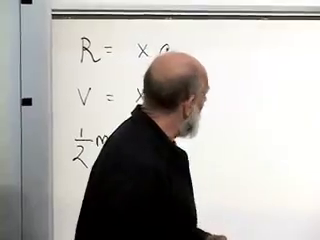
\includegraphics[width=0.72\textwidth]{lecture_09_figure_02.png}
  \caption{La métrica plana en expansión, con el factor de escala multiplicando el elemento de línea espacial euclidiano. Fotograma de la fuente en 00:09:12.}
  \label{fig:l09-expanding-metric-board}
\end{figure}

Imaginemos coordenadas dibujadas sobre una lámina de goma. Las marcas de coordenadas permanecen unidas a la lámina mientras aumenta la distancia física entre ellas. Por tanto, una diferencia de coordenadas como «de \(x=0\) a \(x=1\)» no es más que un par de etiquetas. La distancia que representa ese intervalo es \(a(t)\). Encontrar la ecuación que rige este factor de escala es el problema dinámico de la clase.

\section{Geometrías espaciales cerradas, planas y abiertas}

La planitud es una simplificación observacional, no una consecuencia de la homogeneidad. Hay tres geometrías espaciales homogéneas e isótropas: de curvatura positiva, nula y negativa. Para entender el caso positivo, conviene precisar la dimensión.

El lugar geométrico
\begin{equation}
  X_1^2+X_2^2=R^2
\end{equation}
es un círculo, o una esfera unidimensional \(S^1\). Su interior relleno es un disco, también llamado bola bidimensional. Al añadir una coordenada de inmersión se obtiene
\begin{equation}
  X_1^2+X_2^2+X_3^2=R^2,
\end{equation}
la esfera ordinaria \(S^2\). Al añadir una cuarta coordenada de inmersión se obtiene
\begin{equation}
  X_1^2+X_2^2+X_3^2+X_4^2=R^2,
  \label{eq:l09-three-sphere}
\end{equation}
una esfera tridimensional \(S^3\), que es en sí misma un espacio tridimensional. No podemos visualizar su inmersión en cuatro dimensiones, pero la geometría intrínseca no necesita esa inmersión para existir.

\begin{figure}[H]
  \centering
  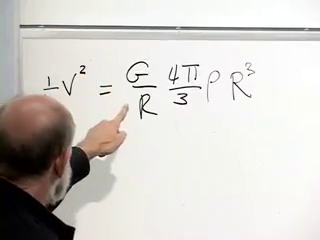
\includegraphics[width=0.72\textwidth]{lecture_09_figure_03.png}
  \caption{La ecuación de inmersión empleada para introducir la esfera tridimensional. Fotograma de la fuente en 00:16:40.}
  \label{fig:l09-three-sphere-board}
\end{figure}

Todos los puntos de una esfera ideal son geométricamente equivalentes, y todas las direcciones en un punto también lo son. Por tanto, una esfera es homogénea e isótropa. Si su radio se multiplica por \(a(t)\), todo el espacio se expande o se contrae sin que se elija un centro en la esfera. Al seguir hacia atrás la evolución de ese universo, no se concentra toda la materia en un lugar especial dentro de un vacío exterior. El espacio entero se hace pequeño, de modo que cada par de puntos se acerca. El Big Bang no es una explosión desde un punto del espacio.

En una esfera de curvatura positiva, la suma de los ángulos de los triángulos geodésicos es mayor que \(180^\circ\). En los triángulos planos, la suma es exactamente \(180^\circ\). En una geometría homogénea de curvatura negativa, representada de manera imperfecta por una silla de montar, la suma es menor que \(180^\circ\). Estas pruebas intrínsecas distinguen los tres casos.

\begin{figure}[H]
  \centering
  \includegraphics[width=0.72\textwidth]{lecture_09_figure_07.png}
  \caption{Curvaturas positiva, nula y negativa ilustradas mediante las formas características de sus triángulos. Fotograma de la fuente en 00:37:30.}
  \label{fig:l09-curvature-board}
\end{figure}

Una métrica local perfectamente plana no demuestra por sí sola que el espacio sea topológicamente infinito. Las topologías planas compactas son matemáticamente posibles, aunque en la clase se adopta el modelo euclidiano infinito más sencillo.
\editorialnote{Esta salvedad sobre la topología global no es necesaria para ninguna de las dinámicas locales que siguen.}

\section{Etiquetas comóviles y ley de Hubble}

Volvamos ahora a la lámina plana en expansión y dibujemos en ella una cuadrícula de coordenadas. En coordenadas comóviles, la cuadrícula se expande junto con el flujo de materia a gran escala. Una galaxia o, más precisamente, un cúmulo de galaxias suficientemente promediado conserva aproximadamente una etiqueta de coordenadas fija, aunque cambie su distancia física respecto de otro objeto comóvil.

\begin{figure}[H]
  \centering
  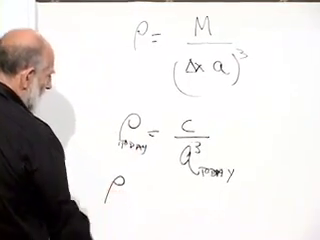
\includegraphics[width=0.72\textwidth]{lecture_09_figure_04.png}
  \caption{Una cuadrícula de coordenadas que acompaña a una lámina espacial en expansión. Fotograma de la fuente en 00:22:20.}
  \label{fig:l09-comoving-grid-board}
\end{figure}

Para dos objetos separados a lo largo del eje \(x\) por un intervalo comóvil fijo \(\Delta x\), su distancia física es
\begin{equation}
  D(t)=a(t)\,\Delta x.
  \label{eq:l09-physical-distance}
\end{equation}
Al derivar manteniendo fijo \(\Delta x\), se obtiene
\begin{equation}
  v(t)=\dot a(t)\,\Delta x
      =\frac{\dot a(t)}{a(t)}D(t).
\end{equation}
Si definimos
\begin{equation}
  H(t)\equiv\frac{\dot a(t)}{a(t)},
  \label{eq:l09-hubble-parameter}
\end{equation}
obtenemos la ley de Hubble,
\begin{equation}
  v=H(t)D.
  \label{eq:l09-hubble-law}
\end{equation}
La palabra «constante» en «constante de Hubble» significa que es constante en el espacio en un instante cósmico dado. No implica que permanezca constante a lo largo de la historia cósmica.

\begin{figure}[H]
  \centering
  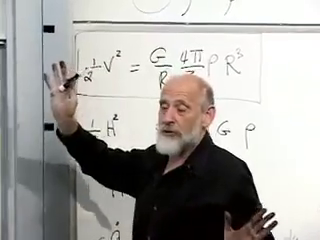
\includegraphics[width=0.72\textwidth]{lecture_09_figure_05.png}
  \caption{La derivación en la pizarra \(D=a\Delta x\),
  \(v=(\dot a/a)D=HD\). Fotograma de la fuente en 00:26:40.}
  \label{fig:l09-hubble-board}
\end{figure}

\begin{classroomqa}\audiencequestion{Si vemos una galaxia distante tal como era en un tiempo anterior, ¿debería su parámetro de Hubble inferido ser realmente igual al valor que medimos hoy en las cercanías?}\lecturerresponse{Solo cuando el tiempo retrospectivo es pequeño en comparación con la edad del universo. A distancias moderadas, \(H(t)\) varía lo bastante poco como para que sea útil un único valor. A distancias verdaderamente cosmológicas observamos épocas anteriores y hay que tener en cuenta la dependencia temporal de \(a\) y \(H\). Esa es una de las razones por las que necesitamos una ecuación dinámica para el factor de escala.}\end{classroomqa}

\section{Rayos nulos en un sistema de coordenadas en expansión}

\begin{classroomqa}\audiencequestion{¿Afecta el factor de escala a la propagación de la luz entre galaxias distantes?}\lecturerresponse{Un rayo de luz sigue una trayectoria nula, así que \(d\tau=0\). Para un rayo que se propaga a lo largo del eje \(x\) positivo, \(dy=dz=0\), y la métrica en expansión da
\begin{align}
  0&=dt^2-a^2(t)dx^2,
  &dt&=a(t)dx,\notag\\
  &&\frac{dx}{dt}&=\frac{1}{a(t)}.
  \label{eq:l09-null-ray}
\end{align}
La velocidad coordenada disminuye a medida que crece \(a(t)\), pero la velocidad física local de la luz sigue siendo \(c=1\). Un intervalo fijo de coordenadas representa una distancia física cada vez mayor.}\end{classroomqa}

\begin{figure}[H]
  \centering
  \includegraphics[width=0.72\textwidth]{lecture_09_figure_06.png}
  \caption{La condición nula y \(dt=a(t)dx\) para la propagación radial de la luz. Fotograma de la fuente en 00:30:54.}
  \label{fig:l09-null-board}
\end{figure}

Se pueden elegir coordenadas en las que este mismo hecho se exprese como «la luz se ralentiza cuanto más lejos está», pero entonces las longitudes y los relojes adquieren descripciones igualmente engorrosas. El lenguaje del espacio en expansión es más claro porque conserva la afirmación local de que todos los observadores en caída libre miden la misma velocidad de la luz.

\begin{classroomqa}\audiencequestion{¿Hay pruebas de que la propagación local de la luz y la física atómica sean iguales en galaxias distantes?}\lecturerresponse{Solo tienen significado operacional las comparaciones adimensionales. Se puede elegir el tamaño de un átomo como unidad de longitud y un período atómico o nuclear como unidad de tiempo, y luego preguntar cuántos de esos períodos necesita la luz para recorrer la longitud elegida. Las observaciones espectrales respaldan la afirmación de que esas razones adimensionales son iguales en regiones distantes. La evidencia es indirecta, pero este es precisamente el tipo de comparación con el que se pone a prueba la uniformidad de las leyes locales.}\end{classroomqa}

Cuando el universo observable era extremadamente pequeño, la luz podía cruzar rápidamente una región física dada, expresada en la unidad correspondiente al tiempo de cruce de la luz. Esto no significa que \(c\) fuera diferente. Significa que la propia región era pequeña.

\section{Una esfera newtoniana dentro del universo}

Pasemos ahora de la cinemática a la dinámica. Situémonos en el origen y tracemos una esfera lo bastante grande para contener muchas galaxias y cúmulos. Elijamos una galaxia en su frontera. En un universo homogéneo, la distribución de masa es esféricamente simétrica a nuestro alrededor, y el teorema de las capas de Newton da dos resultados cruciales:
\begin{enumerate}
  \item toda la materia distribuida esféricamente fuera del radio elegido ejerce una fuerza newtoniana neta nula sobre la galaxia situada en la frontera;
  \item toda la materia dentro de la esfera actúa, para este movimiento radial, como si estuviera concentrada en el centro.
\end{enumerate}
Usamos un sistema de referencia en el que estamos en reposo, de modo que las velocidades y aceleraciones del argumento siguiente se miden respecto de nosotros.

\begin{figure}[H]
  \centering
  \includegraphics[width=0.72\textwidth]{lecture_09_figure_08.png}
  \caption{Construcción basada en el teorema de las capas: nosotros en el centro y una galaxia de prueba en la frontera de una gran esfera homogénea. Fotograma de la fuente en 00:41:10.}
  \label{fig:l09-shell-board}
\end{figure}

\begin{figure}[H]
  \centering
  \begin{tikzpicture}[scale=0.92,>=Latex]
    \draw[thick] (0,0) circle (2.35);
    \fill (0,0) circle (2pt) node[below left] {us};
    \fill (2.35,0) circle (2.2pt) node[right] {test galaxy \(m\)};
    \draw[->,thick,blue!65!black] (0.18,0) -- (2.15,0)
      node[midway,above] {\(R=a(t)x\)};
    \draw[->,thick,red!65!black] (2.35,0.12) -- (3.25,0.12)
      node[midway,above] {\(v=\dot a(t)x\)};
    \node[align=center,text width=7cm] at (0,-2.85)
      {outside shells cancel;\\enclosed mass acts at the center};
  \end{tikzpicture}
  \caption{Reconstrucción limpia de la construcción newtoniana.}
  \label{fig:l09-shell-clean}
\end{figure}

Si la galaxia tiene una coordenada comóvil fija \(x\), su radio físico y su velocidad son
\begin{equation}
  R(t)=x a(t),
  \qquad
  v(t)=x\dot a(t)=H(t)R(t).
  \label{eq:l09-radius-velocity}
\end{equation}
Sea \(M\) la masa encerrada por la esfera y \(m\) la masa de la galaxia de prueba. La energía newtoniana es
\begin{equation}
  E=\frac12 m v^2-\frac{GMm}{R}.
  \label{eq:l09-newtonian-energy}
\end{equation}

\begin{figure}[H]
  \centering
  \includegraphics[width=0.72\textwidth]{lecture_09_figure_09.png}
  \caption{La secuencia completa de la pizarra: \(R=xa\), \(v=x\dot a\) y la ecuación de la energía newtoniana particularizada para \(E=0\). Fotograma de la fuente en 00:48:40.}
  \label{fig:l09-energy-board}
\end{figure}

La energía puede ser positiva, nula o negativa. Empecemos por el límite entre el escape y el colapso, \(E=0\), para el cual
\begin{equation}
  \frac12 v^2=\frac{GM}{R}.
  \label{eq:l09-zero-energy}
\end{equation}

\begin{classroomqa}\audiencequestion{¿Qué significa que la energía total sea nula para la galaxia que se aleja?}\lecturerresponse{Es exactamente el caso de la velocidad de escape. Una energía positiva significa un movimiento por encima de la velocidad de escape; una energía negativa, un movimiento por debajo de ella y, en el modelo newtoniano con solo materia, un retorno eventual. Empezamos en el límite entre esas posibilidades y volveremos a los otros signos después de derivar la ecuación plana.}\end{classroomqa}

\begin{classroomqa}\audiencequestion{¿Varía la masa encerrada \(M\) a medida que se expande la esfera?}\lecturerresponse{No. La esfera es comóvil, así que las mismas partículas permanecen en su interior. Su volumen físico crece y su densidad disminuye, pero la masa total encerrada permanece fija. Esta distinción entre \(M\) y \(\rho(t)\) es esencial.}\end{classroomqa}

Para una densidad homogénea \(\rho(t)\),
\begin{equation}
  M=\frac{4\pi}{3}\rho(t)R^3.
  \label{eq:l09-enclosed-mass}
\end{equation}
Al sustituir en \eqref{eq:l09-zero-energy} se obtiene
\begin{equation}
  \frac12 v^2
  =\frac{G}{R}\left(\frac{4\pi}{3}\rho R^3\right).
  \label{eq:l09-enclosed-energy}
\end{equation}

\begin{figure}[H]
  \centering
  \includegraphics[width=0.72\textwidth]{lecture_09_figure_10.png}
  \caption{Sustitución de la masa encerrada en la ecuación de energía nula. Fotograma de la fuente en 00:54:16.060.}
  \label{fig:l09-enclosed-mass-board}
\end{figure}

Usando \(v=HR\), encontramos
\begin{align}
  \frac12 H^2R^2
    &=\frac{4\pi G}{3}\rho R^2,\\
  H^2
    &=\frac{8\pi G}{3}\rho.
\end{align}
Así, la ley de expansión espacialmente plana con energía nula es
\begin{equation}
  \boxed{\left(\frac{\dot a}{a}\right)^2
  =\frac{8\pi G}{3}\rho(t)}.
  \label{eq:l09-flat-friedmann}
\end{equation}
La cancelación de \(R^2\) no es accidental. En un universo homogéneo, \(H(t)\) debe tener el mismo valor, sea cual sea la galaxia comóvil elegida como objeto de prueba.

\begin{figure}[H]
  \centering
  \includegraphics[width=0.72\textwidth]{lecture_09_figure_11.png}
  \caption{La cancelación del radio y la relación de Friedmann plana resultante en la pizarra. Fotograma de la fuente en 00:57:30.}
  \label{fig:l09-friedmann-board}
\end{figure}

\begin{classroomqa}\audiencequestion{¿Hay pruebas de la relación de energía nula?}\lecturerresponse{Ambos lados pueden inferirse observacionalmente: \(H\) a partir de los datos de recesión y \(\rho\) contabilizando estrellas, gas, materia oscura y energía del vacío. La comparación en la época de la clase encontró que ambos lados concordaban con una precisión aproximada del uno por ciento. La salvedad es importante: hay que incluir todas las formas de energía, y el análisis posterior de la energía del vacío modifica la interpretación ingenua en términos de la velocidad de escape.}\end{classroomqa}

En unidades \(c=1\), la densidad de masa y la densidad de energía tienen las mismas unidades. Por tanto, el símbolo \(\rho\) denotará la densidad de energía total pertinente para el componente considerado.

\section{Materia ordinaria y ley de dos tercios}

La ecuación \eqref{eq:l09-flat-friedmann} no queda cerrada hasta que sepamos cómo cambia \(\rho(t)\). Primero llenemos una caja rectangular comóvil con partículas no relativistas que se mueven lentamente. Sus dimensiones en coordenadas son fijas, mientras que su volumen físico crece como
\begin{equation}
  V(t)=a^3(t)\,\Delta x\,\Delta y\,\Delta z.
\end{equation}
El número de partículas y la masa en reposo dentro de la caja permanecen fijos, así que
\begin{equation}
  \rho_{\mathrm m}(t)=\frac{C_{\mathrm m}}{a^3(t)}.
  \label{eq:l09-matter-dilution}
\end{equation}
Normalizando respecto de la época actual \(t_0\),
\begin{equation}
  \frac{\rho_{\mathrm m}(t)}{\rho_{\mathrm m,0}}
  =\left(\frac{a_0}{a(t)}\right)^3.
  \label{eq:l09-matter-normalized}
\end{equation}

\begin{figure}[H]
  \centering
  \includegraphics[width=0.72\textwidth]{lecture_09_figure_12.png}
  \caption{Densidad de materia, su dilución \(a^{-3}\) y normalización al valor actual. Fotograma de la fuente en 01:04:47.940.}
  \label{fig:l09-density-board}
\end{figure}

\begin{classroomqa}\audiencequestion{¿Cuál es el orden de magnitud aproximado de la densidad de energía actual del universo, y pueden aportarla por sí solos los átomos ordinarios?}\lecturerresponse{Un recuento de la materia bariónica visible solo da parte de la respuesta. La materia oscura y la energía oscura también deben representarse como masa-energía equivalente. La clase cita una escala aproximada que va desde un átomo hasta unas pocas decenas de equivalentes de masa del hidrógeno por metro cúbico, haciendo hincapié en el orden de magnitud y no en un inventario preciso.}\end{classroomqa}

Sustituyamos \eqref{eq:l09-matter-dilution} en
\eqref{eq:l09-flat-friedmann} y absorbamos en una constante positiva \(C\) todos los factores independientes del tiempo:
\begin{equation}
  \left(\frac{\dot a}{a}\right)^2=\frac{C}{a^3},
  \qquad
  \dot a^2=\frac{C}{a}.
  \label{eq:l09-matter-ode}
\end{equation}
Hay dos maneras claras de resolverla. Una solución de prueba en forma de ley de potencias, \(a=K t^p\), exige que
\begin{equation}
  p-1=-\frac{p}{2},
  \qquad p=\frac23.
\end{equation}
De manera equivalente, tomemos la rama positiva de la raíz cuadrada, correspondiente a la expansión, e integremos:
\begin{equation}
  a^{1/2}\frac{da}{dt}=\sqrt C,
  \qquad
  \int a^{1/2}da=\sqrt C\int dt,
\end{equation}
por lo que, al elegir el origen temporal del Big Bang,
\begin{equation}
  a^{3/2}\propto t,
  \qquad
  \boxed{a(t)\propto t^{2/3}}.
  \label{eq:l09-matter-solution}
\end{equation}
En la derivación en directo se pierde brevemente un factor al ajustar los coeficientes; luego se vuelve a la integral y se comprueba el exponente. Los apuntes conservan la comprobación, pero muestran solo el álgebra corregida.

\begin{figure}[H]
  \centering
  \includegraphics[width=0.72\textwidth]{lecture_09_figure_13.png}
  \caption{La solución de prueba en forma de ley de potencias y el exponente enmarcado \(p=2/3\). Fotograma de la fuente en 01:13:05.}
  \label{fig:l09-matter-solution-board}
\end{figure}

Al derivar la solución se obtiene
\begin{equation}
  H(t)=\frac{\dot a}{a}=\frac{2}{3t}.
  \label{eq:l09-matter-hubble}
\end{equation}
El parámetro de Hubble era mayor en el pasado. Por consiguiente, si miramos lo bastante lejos como para observar un tiempo retrospectivo apreciable, no deberíamos prolongar la relación lineal local usando sin cambios el valor actual de \(H_0\).

\begin{figure}[H]
  \centering
  \includegraphics[width=0.72\textwidth]{lecture_09_figure_14.png}
  \caption{Tomar \(\dot a/a\) para \(a\propto t^{2/3}\) da
  \(H=2/(3t)\). Fotograma de la fuente en 01:20:42.}
  \label{fig:l09-hubble-time-board}
\end{figure}

\section{El signo de la energía y la curvatura espacial}

El razonamiento newtoniano nos ha llevado hasta el caso plano de energía nula. La relatividad general añade un hecho que no se puede obtener solo del teorema de las capas: el signo de la energía específica de tipo newtoniano corresponde al signo de la curvatura espacial.
\begin{center}
\begin{tabular}{@{}>{\raggedright\arraybackslash}p{0.20\linewidth}
                    >{\raggedright\arraybackslash}p{0.29\linewidth}
                    >{\raggedright\arraybackslash}p{0.37\linewidth}@{}}
  \toprule
  Energía total & Curvatura espacial & Evolución con solo materia \\
  \midrule
  positiva & negativa (abierta) &se expande para siempre \\
  nula &nula (plana) &se aproxima al límite de escape \\
  negativa &positiva (cerrada) &se expande, alcanza un máximo y vuelve a colapsar \\
  \bottomrule
\end{tabular}
\end{center}
La última columna supone que no hay energía del vacío. En la analogía del proyectil, una energía positiva significa superar la velocidad de escape; una energía nula, alcanzarla exactamente; y una energía negativa, quedar por debajo de ella. Las ecuaciones de Einstein identifican estos tres casos, respectivamente, con geometrías espaciales abiertas, planas y cerradas.

\section{Fotones y ley de un medio}

La ley de la materia \(\rho\propto a^{-3}\) supone que la energía de cada partícula es aproximadamente fija mientras disminuye la densidad numérica. Los fotones no cumplen esa hipótesis. Para un fotón,
\begin{equation}
  E=h\nu=\frac{hc}{\lambda}.
\end{equation}
La expansión estira su longitud de onda en proporción al factor de escala,
\begin{equation}
  \lambda\propto a,
  \qquad E\propto a^{-1}.
\end{equation}
La densidad numérica de fotones sigue disminuyendo como \(a^{-3}\), y la energía de cada fotón aporta un factor adicional de \(a^{-1}\). Por tanto,
\begin{equation}
  \boxed{\rho_{\mathrm r}(t)\propto a^{-4}(t)}.
  \label{eq:l09-radiation-dilution}
\end{equation}

La analogía de la cuerda de guitarra ilustra la situación física. Se pulsa una cuerda y luego se alarga el tramo que vibra: la longitud de onda aumenta y el tono se vuelve más grave. Un modo de fotón en una caja comóvil en expansión se comporta de forma similar. Si se sigue la evolución hacia atrás, la compresión acorta las longitudes de onda y eleva las energías de los fotones.

\begin{figure}[H]
  \centering
  \includegraphics[width=0.72\textwidth]{lecture_09_figure_15.png}
  \caption{La relación de la densidad de materia ampliada en la pizarra hasta la ley de escala de la radiación \(\rho_{\mathrm r}\propto a^{-4}\). Fotograma de la fuente en 01:29:20.}
  \label{fig:l09-radiation-board}
\end{figure}

Al usar \(\rho_{\mathrm r}\propto a^{-4}\) en la ecuación de Friedmann plana, se obtiene
\begin{equation}
  \left(\frac{\dot a}{a}\right)^2=\frac{C_{\mathrm r}}{a^4},
  \qquad
  \dot a\propto a^{-1},
\end{equation}
y, por tanto,
\begin{equation}
  \boxed{a(t)\propto t^{1/2}}.
  \label{eq:l09-radiation-solution}
\end{equation}
Esto crece más lentamente que \(t^{2/3}\). Si retrocedemos lo suficiente en el tiempo, la radiación necesariamente domina sobre la materia ordinaria, porque \(a^{-4}\) aumenta más rápidamente que \(a^{-3}\) cuando \(a\) disminuye. La clase sitúa la transición entre el dominio de la radiación y el de la materia aproximadamente en la época en que el factor de escala era unas mil veces menor que hoy. Antes de esa transición dominaba la radiación; después, durante un largo intervalo, dominó la materia.

\section{Energía del vacío y expansión exponencial}

La energía del vacío tiene un comportamiento de escala opuesto. Su densidad es una propiedad del espacio vacío y no se diluye al expandirse el universo:
\begin{equation}
  \rho_\Lambda=\text{constant}.
  \label{eq:l09-vacuum-density}
\end{equation}
La materia ordinaria y la radiación se vuelven más densas hacia el pasado, mientras que este término no lo hace. Por eso tenía menos importancia en el universo temprano y cobra más importancia a medida que se diluyen los demás componentes. La clase utiliza la estimación entonces vigente según la cual la energía del vacío aporta aproximadamente \(70\%\) de la densidad de energía cósmica actual.

Con \(\rho_\Lambda\) constante, la ecuación \eqref{eq:l09-flat-friedmann} da una tasa de expansión constante
\begin{equation}
  H_\Lambda=\sqrt{\frac{8\pi G}{3}\rho_\Lambda},
  \qquad
  \frac{\dot a}{a}=H_\Lambda.
\end{equation}
Por tanto,
\begin{equation}
  \boxed{a(t)=a(t_i)e^{H_\Lambda(t-t_i)}}.
  \label{eq:l09-vacuum-solution}
\end{equation}

\begin{figure}[H]
  \centering
  \includegraphics[width=0.72\textwidth]{lecture_09_figure_16.png}
  \caption{La ecuación de densidad constante que conduce a la expansión exponencial. Fotograma de la fuente en 01:35:48.}
  \label{fig:l09-vacuum-board}
\end{figure}

A la escala observada citada en la clase, el universo duplica su tamaño lineal en unos diez a doce mil millones de años. El origen de esta pequeña pero no nula densidad del vacío sigue sin explicación; su existencia y su efecto sobre la expansión son hechos empíricos.

\begin{classroomqa}\audiencequestion{¿En este análisis, la energía del vacío es lo mismo que la energía oscura?}\lecturerresponse{Sí. Aquí, «energía oscura» designa una densidad de energía del vacío constante, equivalente a una constante cosmológica. Se pueden imaginar modelos más generales de energía oscura que varíe con el tiempo, pero no forman parte de los cálculos de esta clase.}\end{classroomqa}

\section{Cómo el universo en expansión desplaza al rojo la luz}

\begin{classroomqa}\audiencequestion{¿Cómo pueden saber los fotones que hemos elegido coordenadas comóviles en expansión y, por eso, reducir su energía?}\lecturerresponse{No responden a nuestras etiquetas. Se propagan por una geometría en la que cambian las distancias físicas. Un tren de ondas que ocupa una región cuyo tamaño físico se duplica adquiere el doble de longitud de onda. Las coordenadas comóviles simplemente describen ese estiramiento de manera económica; no lo causan.}\end{classroomqa}

\begin{classroomqa}\audiencequestion{¿De dónde provienen los fotones de fondo que nos llegan hoy?}\lecturerresponse{Mirar más lejos es mirar hacia épocas anteriores. Al final llegamos a la época en que el material cósmico era un plasma ionizado, opaco porque los fotones se dispersaban repetidamente en partículas cargadas libres. La frontera desde la que los fotones pudieron viajar libremente hasta nosotros por última vez aparece como una esfera que rodea al observador: la superficie de última dispersión.}\end{classroomqa}

\begin{figure}[H]
  \centering
  \includegraphics[width=0.72\textwidth]{lecture_09_figure_17.png}
  \caption{Esquema centrado en el observador de la superficie de última dispersión y de capas cada vez más distantes. Fotograma de la fuente en 01:42:05.}
  \label{fig:l09-last-scattering-board}
\end{figure}

\begin{figure}[H]
  \centering
  \begin{tikzpicture}[scale=0.9,>=Latex]
    \fill (0,0) circle (2pt) node[below] {observer};
    \draw[thick,orange!70!black] (0,0) circle (2.55);
    \node[orange!70!black,align=center] at (0,3.05)
      {surface of last scattering};
    \foreach \a in {25,75,145,210,285,335}{
      \draw[->,blue!60!black] ({2.55*cos(\a)},{2.55*sin(\a)}) --
        ({1.7*cos(\a)},{1.7*sin(\a)});
    }
    \draw[decorate,decoration={snake,amplitude=1.5pt,segment length=7pt},
      red!65!black,thick,->] (-2.5,0) -- (-0.15,0);
    \node[red!65!black,below] at (-1.35,-0.15)
      {redshifted photon};
  \end{tikzpicture}
  \caption{Reconstrucción limpia de la imagen de la última dispersión.}
  \label{fig:l09-last-scattering-clean}
\end{figure}

La radiación se emitió con un espectro característico de un plasma caliente y nos llega con longitudes de onda aproximadamente mil veces mayores. En el lenguaje Doppler de la clase, la superficie emisora distante se aleja rápidamente y su radiación experimenta un intenso desplazamiento al rojo. En términos geométricos, la onda se estira durante su propagación. Ambas descripciones codifican la misma relación,
\begin{equation}
  1+z=\frac{\lambda_0}{\lambda_{\mathrm{em}}}
      =\frac{a_0}{a_{\mathrm{em}}}.
  \label{eq:l09-cosmological-redshift}
\end{equation}
\editorialnote{La ecuación \eqref{eq:l09-cosmological-redshift} es la forma cuantitativa estándar de las descripciones de estiramiento y efecto Doppler empleadas en la clase.}

En una época de observación anterior, la esfera de última dispersión habría estado más cerca en la imagen correspondiente, y los fotones de fondo observados habrían sufrido un menor desplazamiento al rojo y, por tanto, habrían tenido más energía. A medida que avanza el tiempo cósmico, los fotones que llegan a un observador comóvil desde aquel plasma temprano tienen longitudes de onda cada vez mayores.

\section{¿Adónde va la energía de un fotón desplazado al rojo?}

\begin{classroomqa}\audiencequestion{Un fotón se emite con una energía \(h\nu_{\mathrm{em}}\) y llega con desplazamiento al rojo y menos energía. ¿Qué ocurrió con la diferencia?}\lecturerresponse{La derivación newtoniana comenzó como una ecuación de energía. Su forma cosmológica relaciona la tasa de expansión con la densidad de energía de la materia, así que no se pueden tratar la energía de la materia y la expansión como magnitudes conservadas por separado. La clase describe la energía perdida por el fotón como incorporada al balance cinético de la expansión. Un pistón lleno de radiación concreta la analogía: la presión de radiación empuja el pistón hacia fuera, las longitudes de onda de los fotones aumentan y la energía que pierden se convierte en trabajo mecánico y energía cinética del pistón.}\end{classroomqa}

\begin{figure}[H]
  \centering
  \includegraphics[width=0.72\textwidth]{lecture_09_figure_18.png}
  \caption{La pizarra sitúa la ecuación newtoniana de la energía, enmarcada, encima de la ecuación de Friedmann correspondiente. Fotograma de la fuente en 01:44:42.}
  \label{fig:l09-energy-bookkeeping-board}
\end{figure}

\begin{classroomqa}\audiencequestion{¿Qué acopla la energía de la radiación a la expansión?}\lecturerresponse{La presión. En un cilindro con un pistón móvil, los fotones transfieren momento a la pared. Cuando el pistón se mueve, la radiación realiza trabajo; su longitud de onda aumenta y su energía disminuye. El universo homogéneo en expansión no tiene un pistón exterior literal, pero la analogía de \(p\,dV\) explica por qué la densidad de energía de la radiación disminuye más rápidamente de lo que bastaría la mera dilución numérica.}\end{classroomqa}

\begin{figure}[H]
  \centering
  \includegraphics[width=0.72\textwidth]{lecture_09_figure_19.png}
  \caption{El pistón móvil lleno de fotones que se usa para visualizar el trabajo de la presión. Fotograma de la fuente en 01:46:40.}
  \label{fig:l09-piston-board}
\end{figure}

\begin{figure}[H]
  \centering
  \begin{tikzpicture}[scale=0.92,>=Latex]
    \draw[thick] (0,0) rectangle (5.3,2.6);
    \draw[very thick] (4.25,0) -- (4.25,2.6);
    \draw[very thick] (4.25,1.3) -- (5.25,1.3);
    \draw[->,thick,red!65!black] (5.25,1.3) -- (6.2,1.3)
      node[right] {moving piston};
    \foreach \y in {0.55,1.3,2.05}{
      \draw[decorate,decoration={snake,amplitude=1.4pt,segment length=6pt},
        blue!65!black,->] (0.35,\y) -- (3.9,\y);
    }
    \node at (2.15,-0.45) {radiation does \(p\,dV\) work};
  \end{tikzpicture}
  \caption{Reconstrucción limpia de la analogía del pistón con radiación.}
  \label{fig:l09-piston-clean}
\end{figure}

La energía en relatividad general exige cautela. En un espacio-tiempo genérico en expansión no tiene por qué existir una energía global conservada única, análoga a la energía de un sistema newtoniano aislado. La conservación local del tensor de energía-momento sigue cumpliéndose y, para un fluido homogéneo, da lugar a la ecuación de continuidad
\begin{equation}
  \dot\rho+3H(\rho+p)=0,
  \label{eq:l09-continuity}
\end{equation}
que contiene el término de trabajo de presión que subyace a las leyes de escalamiento de la materia y la radiación.\editorialnote{La ecuación \eqref{eq:l09-continuity} es la formulación local precisa de la relatividad general que fundamenta la analogía deliberadamente newtoniana de la clase para llevar la contabilidad de la energía.}

La energía del vacío vuelve especialmente agudo el problema. Como su densidad permanece constante mientras el volumen crece, la energía total del vacío en una región comóvil aumenta. Su presión negativa forma parte de la fuente gravitatoria e impulsa la expansión acelerada. Por lo tanto, no se debe exigir la conservación por separado de la ingenua «energía de la materia en una caja comóvil» sin tener en cuenta la geometría y el trabajo de presión.

\section{Por qué se puede eliminar el factor de escala del término temporal}

\begin{classroomqa}
\audiencequestion{¿Por qué el factor de escala multiplica la parte espacial de la métrica, pero no la parte temporal?}
\lecturerresponse{Se trata de una elección de coordenada temporal. Supongamos que se parte de una coordenada de tiempo conforme \(t\), con
\begin{equation}
  d\tau^2=A^2(t)\left(dt^2-dx^2\right).
\end{equation}
Definamos un nuevo tiempo cósmico \(T\) mediante
\begin{equation}
  dT=A(t)\,dt.
\end{equation}
Entonces
\begin{equation}
  d\tau^2=dT^2-A^2\bigl(t(T)\bigr)dx^2.
\end{equation}
El factor común delante del diferencial temporal ha desaparecido, mientras que el factor de escala físico permanece en el término espacial.}
\end{classroomqa}

\begin{figure}[H]
  \centering
  \includegraphics[width=0.72\textwidth]{lecture_09_figure_20.png}
  \caption{La redefinición del tiempo \(dT=A(t)dt\) que convierte el tiempo conforme en tiempo cósmico. Fotograma de la fuente en 01:51:05.}
  \label{fig:l09-time-reparam-board}
\end{figure}

\section{Curvatura, energía del vacío y destino cósmico}

\begin{classroomqa}
\audiencequestion{Si el universo tuviera curvatura positiva, ¿deberíamos ver ya galaxias que se acercan a nosotros?}
\lecturerresponse{No necesariamente. Un proyectil lanzado por debajo de la velocidad de escape primero se aleja, alcanza un punto de retorno y solo después cae de vuelta. Observamos el universo durante una fase de expansión. Sin energía del vacío, un universo de materia con curvatura positiva acabaría colapsando de nuevo. Una energía del vacío positiva suficientemente grande impide ese punto de retorno, y el valor observado parece lo bastante grande como para que la expansión a largo plazo sea exponencial, independientemente de una pequeña curvatura espacial.}
\end{classroomqa}

El futuro exponencial no es un paraíso energético. Las estrellas acabarán apagándose, las densidades de materia y radiación disminuirán exponencialmente y regiones distantes quedarán fuera del contacto causal. La energía del vacío permanece mientras las estructuras ordinarias se vuelven progresivamente más frías y menos densas.

\begin{classroomqa}
\audiencequestion{Al mirar más atrás en el tiempo, ¿había más fotones que partículas ordinarias?}
\lecturerresponse{La razón entre el número de fotones y el de bariones ya es enorme: según la estimación de la clase, aproximadamente \(10^{10}\) fotones por barión. Ambos números permanecen aproximadamente constantes en un volumen comóvil. Lo que cambia al retroceder en el tiempo es, sobre todo, la energía de cada fotón. Las energías de los fotones aumentan como \(a^{-1}\), mientras que las masas en reposo no relativistas no cambian. Por eso la radiación domina la densidad de energía en los primeros tiempos, aunque la propia razón entre los números no tenga por qué cambiar.}
\end{classroomqa}

La lección central es que la geometría por sí sola no determina la historia cósmica. La ecuación de Friedmann para un universo plano establece la relación entre la expansión y la densidad de energía, pero el contenido material determina cómo evolucionan con el tiempo. La materia no relativista da \(a\propto t^{2/3}\), la radiación da \(a\propto t^{1/2}\) y la energía constante del vacío produce una expansión exponencial. Esas tres leyes ordenan las sucesivas eras del universo y explican por qué el mismo factor de escala rige las distancias, los corrimientos al rojo y la evolución del parámetro de Hubble.

\end{document}
